%% ===================================================================
%% main.tex — Artificial Intelligence and Law (Springer), double-blind.
%%
%% EVERY NUMBER comes from docs/research/RESULTS.md, whose tables are
%% generated from artifacts by `pipeline run results` and verified with
%% `--flag check=true`. No figure in this file is hand-maintained.
%%
%% Numbers from the retired study must never appear here — see
%% the forbidden-numbers table in docs/paper/PAPER-MAP.md §0.
%% ===================================================================

\documentclass[sn-mathphys-num]{sn-jrnl}      % Springer Nature template
%\documentclass[11pt]{article}                % FALLBACK: flip these two lines

\makeatletter
\@ifclassloaded{sn-jrnl}{%
}{%
  \usepackage[round,authoryear]{natbib}
  \bibliographystyle{plainnat}
  \newcommand{\fnm}[1]{#1}\newcommand{\sur}[1]{#1}
  \newcommand{\orgname}[1]{#1}\newcommand{\orgdiv}[1]{#1}%
  \newcommand{\orgaddress}[1]{#1}\newcommand{\city}[1]{#1}\newcommand{\country}[1]{#1}
  \newcommand{\affil}[2][]{}
  \let\snfallback@title\title
  \renewcommand{\title}[2][]{\snfallback@title{#2}}
  \let\snfallback@author\author
  \renewcommand{\author}[2][]{\snfallback@author{#2}}
  \def\snfallback@abs{}\long\def\abstract#1{\long\def\snfallback@abs{#1}}
  \def\snfallback@kw{}\newcommand{\keywords}[1]{\def\snfallback@kw{#1}}
  \let\snfallback@maketitle\maketitle
  \renewcommand{\maketitle}{\snfallback@maketitle
    \begin{quote}\small\noindent\textbf{Abstract.}\ \snfallback@abs\par\medskip
    \noindent\textbf{Keywords:}\ \snfallback@kw\end{quote}}
}
\makeatother

\usepackage{graphicx}
\usepackage{booktabs}
\usepackage{amsmath}
\usepackage{amssymb}
\usepackage{url}
\usepackage{longtable}
\graphicspath{{figures/}{../figures/}}

\title[Modelling administrative process types and typical paths]{Modelling administrative
process types and typical paths from an event log: an auditable catalogue for administrative
transparency and optimisation}

%% DOUBLE-BLIND: no names, no affiliation, no identifying sigla.
\author[1]{\fnm{Anonymous} \sur{Authors}}
\affil[1]{\orgname{Anonymised for double-blind review}, \country{Brazil}}

\abstract{Access-to-information law presumes that public administrations hold an account of how
their procedures actually run. Empirical work on open-records requests finds that this account
is frequently absent: the binding obstacle is not exemption but that the record was never
created. We derive such a record from an administration's own event log. From 5{,}243 concluded
administrative cases at a state-level secretariat of a Brazilian state administration, we build
an event knowledge graph, group cases into emergent process types from opening-document text
together with routing and action history, and learn a typical path for each type using
sequence models over two trace alphabets: recorded actions, and the itinerary of organisational
units a case visits. The catalogue is reproducible --- every clustering refittable from a feature
matrix reproduces exactly from its stamped features, every reported table is regenerated from
artefacts, and a register of the load-bearing figures in the running text is checked against
those artefacts in both directions. Evaluating it required controls that this
literature does not routinely report. A shuffled partition, preserving cluster count, size
distribution and evaluated population, reduces next-step accuracy from 0.726 to 0.494,
establishing that the grouping carries signal. What per-cluster modelling then contributes
depends on how it is measured, and the conventional measurement overstates it roughly sixfold.
Against the usual within-cluster baseline the apparent gain on action prediction is 0.083;
against a single global model with the model family held fixed it is 0.004; and once both trace
alphabets are scored on one population it is negative, between $-0.009$ and $-0.005$ depending
on whether clusters are weighted by membership or by prediction steps. Routing gains 0.029 to
0.036 on the same population and under the same choice. Two further results constrain the
method: sixteen clusterings across four algorithm families fall within 0.0079 once scored on a
common set of cases, on an interval too wide to call them equivalent; and the internal validity
indices that would ordinarily choose between them track cluster granularity rather than
downstream utility, correlating at 0.87 with median cluster size while their association with
accuracy cannot be resolved at this sample size. Anonymisation applied before clustering, as the
governing instrument requires, costs no measurable next-activity utility against a pre-registered
margin.}

\keywords{process mining, administrative transparency, trace clustering, access to information,
data protection, public administration}


\begin{document}
\maketitle

\section{Introduction}\label{sec:intro}

Access-to-information law assumes that public administrations know how they work. Freedom of
information regimes, open data mandates and machine-readable publication duties are all written
as though an accurate account of administrative practice sits somewhere in a filing system,
waiting to be released. \citet{brauneis2018algorithmic} tested that assumption directly, filing
42 open-records requests across 23 states, and found the binding obstacle was not trade secrecy
or exemption. It was that the records had never been created. There was nothing to disclose.

Administrative process systems make the gap partially solvable. A modern electronic process
system records every action taken on every case: which unit received it, what was done, when it
moved on. The trace exists. What does not exist is the account of what those traces mean in
aggregate: which kinds of procedure the administration actually runs, and how each of them
actually flows. Administrations do maintain a declared taxonomy of procedure types, but that
taxonomy is a classification applied at opening, by the person opening the case, and its
relationship to observed practice is an empirical question rather than a given.

In the corpus studied here, that relationship is weak in a specific and diagnosable way. A
single catch-all label covers 30.5\% of the concluded cases. Compare an emergent partition derived from the
event log against the declared taxonomy and the agreement is modest (ARI 0.202); remove that one
label and agreement rises to 0.352. The official taxonomy is not uninformative everywhere. Its
disagreement with practice is concentrated in a junk drawer, which is the characteristic failure
of a classification maintained for filing rather than for analysis.

This paper derives the missing record and shows how such a record has to be evaluated. From the
event log of a state-level secretariat of a Brazilian state administration, we build an event
knowledge graph of 5{,}243 concluded administrative cases, group them into emergent process
types using the text of each case's opening document together with its routing and action
history, and learn a typical path for each type. The result is a catalogue: a set of named
process types, each with a representative flow, derived from the administration's own records
and regenerable from them.

\subsection*{Contributions}

\textbf{An auditable as-is catalogue of process types, offered as a transparency instrument.}
The artefact is what the machine-readable publication duty in Brazil's access-to-information
law contemplates, and what \citeauthor{brauneis2018algorithmic}'s requesters could not obtain.
Two properties make it usable rather than merely produced. It is non-random: permuting cluster
membership while holding cluster count, size distribution and evaluated population fixed drops
downstream next-step accuracy from 0.726 to 0.494, so the grouping carries the signal rather
than the shape of the partition. And it is reproducible: every clustering that is defined as a function of the feature matrix refits exactly
from its stamped feature matrix, and every number reported in this paper is regenerated from
artefacts by a pipeline stage that fails if a generated table drifts, and the load-bearing
figures in the running text are held to the artefacts by a second check that fails in either
direction.

\textbf{An external evaluation protocol, with controls, for judging such a catalogue.} The
principle of scoring a clustering by the downstream model it enables is established
\citep{deweerdt2013actitrac}; we extend it from process-model fitness to next-activity
prediction, apply it externally to partitions produced independently by four algorithm families
across two trace alphabets, and add two controls this literature does not routinely report. The
controls matter more than the extension. Measured against the conventional within-cluster
baseline, per-cluster modelling appears to gain 0.083; measured against a single global model
trained on the pooled corpus, the gain is 0.013. Both numbers are correct measurements of
different quantities, and reporting only the first is what makes a modest result look strong.

The two contributions are deliberately independent. The catalogue claim rests on the shuffled
control and on reproducibility, not on the size of the downstream gain, so the modest gain does
not undercut it.

\subsection*{Research questions}

\begin{description}
  \item[RQ1] Can an auditable catalogue of emergent process types be derived from the event log
    and opening-document text, and does it capture structure the declared taxonomy misses?
  \item[RQ2] Does the choice of clustering algorithm matter to downstream utility, and do
    internal cluster validity indices predict it --- or do they measure something else?
  \item[RQ3] Do per-cluster typical paths generalise --- covering what real cases do without
    fabricating steps --- and do they improve on a global model, a random partition, and a real
    representative case?
  \item[RQ4] Does constrained decoding provide the compliance guarantee an audit artefact
    requires, and at what cost?
  \item[RQ5] Does anonymisation degrade the structure or its downstream utility?
\end{description}

Several answers are negative, and they are reported as findings. Algorithm choice separates the
clusterings very little: sixteen spanning four algorithm families fall within 0.0079 of each
other once scored on the cases all of them evaluate, though the interval around that spread is
too wide for an equivalence claim. The internal validity indices that would ordinarily choose
between them measure something else: silhouette tracks how much of the corpus a partition
retains, and has no association with accuracy once cluster size is held fixed. A real
representative case remains a strong baseline that the generated paths do not dominate. These results constrain what the method can claim, and they
are the reason the positive results are credible.

Section~\ref{sec:related} situates the work; Section~\ref{sec:legal} sets out the normative
framing; Sections~\ref{sec:method} and \ref{sec:setup} describe the corpus, the method and the
experimental design; Section~\ref{sec:results} reports results by research question;
Sections~\ref{sec:discussion}--\ref{sec:conclusion} discuss, bound and conclude.

\section{Related work}\label{sec:related}

\subsection{Trace clustering}\label{subsec:rw-clustering}

Mining a single model from a heterogeneous log yields a structure that describes no actual
behaviour, and the established remedy is to partition the log first and discover a specialised
model for each group \citep{greco2006clustering}. Partitioning needs a representation. Trace
profiles over activities, transitions, originators and case attributes make vector-space
clustering applicable to event data, and different profiles yield materially different partitions
\citep{song2009trace}; features built from conserved subsequences restore the order information
that bag-of-activities profiles discard \citep{bose2009context}; learned dense representations of
activities and traces outperform hand-crafted profiles on the same task
\citep{dekoninck2018act2vec}. A systematic review organises fifteen years of this work into four
interchangeable dimensions, namely representation, algorithm, use of non-control-flow information,
and evaluation strategy, and it already lists downstream model quality among the recognised
evaluation strategies \citep{zandkarimi2020generic}. The clearest instance is ActiTraC, which
admits a trace into a cluster only when the fitness of the process model discovered for that
cluster does not significantly degrade, so that the downstream artefact drives the grouping rather
than a distance in feature space \citep{deweerdt2013actitrac}. What that literature calls a
variant is close to what we call a process type \citep{taymouri2021variant}.

The difference here is one of placement. ActiTraC uses the downstream score inside the clustering
loop, as a wrapper; we use it afterwards, on partitions that four algorithm families produced
independently over two text arms, which is what allows the question of whether the algorithm
matters at all to be posed. We evaluate emergent process-type partitions by the predictive
performance of per-cluster sequence models, extending the model-driven evaluation principle of
\citet{deweerdt2013actitrac} from process-model fitness to next-activity prediction, and adding
shuffled-partition and global-model controls that this literature does not routinely report.

\subsection{Per-cluster sequence models}\label{subsec:rw-percluster}

Learning one sequence model per cluster is not a recent arrangement. \citet{ferreira2007sequence}
treat clustering as a mixture of first-order Markov chains, so that each cluster \emph{is} a
sequence model and a trace belongs to the cluster whose model most probably generated it;
clustering and per-cluster estimation are a single expectation--maximisation procedure.
\citet{difrancescomarino2019clusteringppm} separate the two stages: prefixes of completed cases
are clustered by control flow, a classifier is trained for each cluster, and a running case is
routed at runtime to the classifier of the cluster it matches. How the sequence is encoded is a
first-order determinant of how such per-cluster predictors perform \citep{teinemaa2019outcome},
and a cross-field comparison of next-element prediction methods finds that the techniques aiming
at interpretable models are the ones that give up accuracy \citep{tax2020interdisciplinary}.

We claim none of this. Our departures are narrow, and each is stated as such: third-order Markov
chains alongside a directly-follows graph and three neural families, rather than a single
first-order chain; complete concluded cases rather than prefixes; a separate extraction step that
turns each per-cluster model into one inspectable path; and, in place of the assumption that the
arrangement pays for itself, a shuffled-partition null and a global-model baseline that measure
how much of the apparent gain survives. Prediction is a measuring instrument here, not the
product.

\subsection{Representative and canonical traces}\label{subsec:rw-representative}

Summarising a cluster by a single execution has formal machinery behind it. Multiple-sequence
alignment, borrowed from bioinformatics, aligns traces column-wise so that the conserved core and
the deviations can be read off directly \citep{bose2012diagnostics}. \citet{chatain2017alignment}
go further and make model traces the centroids of the clusters, so that model explanations of
observed behaviour drive the partition instead of vector-space similarity; later work generalises
the centroid from a single run to a sub-model \citep{boltenhagen2021modelbased}. The idea of one
canonical execution per cluster belongs to that line. A single path is also a deliberate move to
the simplicity corner of the fitness/precision/generalisation/simplicity frame, bought at the cost
of generalisation \citep{buijs2014quality}, and the directly-follows graph we use as one of the
path learners carries its own documented distortions \citep{vanderaalst2019dfg}.

What differs is what the method is allowed to assume. Alignment-based centroids require a process
model as input, and the absence of any documented as-is model is the premise of this study rather
than an inconvenience within it. Our representative is derived from a learned sequence model over
the cluster's own traces, carries a likelihood, is comparable across two trace alphabets and five
model families, and is scored against the medoid of the cluster's real traces, which we report as
the strong baseline it turns out to be. The alignment consensus remains the alternative
representative we did not compute, and we say so where it bears on the interpretation of our
results.

\subsection{Predictive process monitoring and its critiques}\label{subsec:rw-ppm}

Next-activity prediction from event logs is mature. A single recurrent network predicts the next
activity, its timestamp and the remaining case suffix \citep{tax2017lstm}; treating traces as
language licenses the sequence-modelling apparatus wholesale \citep{evermann2017predicting};
attention-based encoders followed \citep{bukhsh2021processtransformer}. The benchmarks matter more
than the architectures. Under a common protocol, reported superiority frequently fails to
reproduce and no architecture dominates across logs \citep{ramamaneiro2023dlppm}, and the splits
in standard use leak information between training and test in ways that inflate reported
performance \citep{weytjens2022leakage}. Both observations are reasons to read a single accuracy
figure as a statement about a particular log and protocol rather than about a method, and they set
the standard of evidence we hold our own comparison to.

The critique we take most seriously is that of \citet{peeperkorn2023rnnstructure}, who show that a
network reaching good next-activity accuracy can still fail to capture the structure of the
underlying process, particularly when generalising to unseen variants. That result shapes our
design rather than threatening it. Fitness and next-activity objectives can disagree, so one
cannot be substituted for the other without argument. We therefore use accuracy retrospectively,
as a measure of how learnable a cluster is, report path-support measures alongside it, and draw no
conclusion about the process itself from an accuracy figure.

\subsection{Cluster validity}\label{subsec:rw-validity}

The indices we compute were introduced as \emph{relative} instruments, that is, devices for
ranking candidate partitions produced under comparable conditions, not absolute measures of
quality \citep{rousseeuw1987silhouettes, daviesbouldin1979measure, calinski1974dendrite,
moulavi2014dbcv}. Read instead as objectives, they misbehave: partitions that directly maximise
popular indices frequently disagree with expert reference labellings \citep{gagolewski2021invalid}.
Over 2.7 million partitions, \citet{yerbury2025rvi} find relative validity indices empirically
unsuitable for choosing between clustering approaches, and recommend outcome-oriented criteria
informed by domain requirements. A further asymmetry bears directly on cross-algorithm
comparison: no established index evaluates whether noise assignments are \emph{correct}, so a
density-based clustering that emits noise and a partitional one that labels every point are not
scored on the same population \citep{beer2026disco}. The genre is familiar from topic modelling,
where a field's consensus intrinsic metric proved negatively correlated with human judgement of
the same models \citep{chang2009teahaves}, and from the argument that clustering admits no
application-independent quality procedure at all \citep{vonluxburg2012clustering}.

The counter-case is \citet{chicco2025dbcv}, who find DBCV more informative than three competing
density-based indices on synthetic data and on health records. We do not contest that finding. It
compares indices within one paradigm on recovery of cluster geometry, where agreement with an
external index reached 60\%, and informativeness about geometry is a different quantity from
predictiveness of downstream utility. Our contribution to this thread is an instance rather than a
theory: sixteen partitions of one administrative corpus, with the indices and a downstream measure
reported side by side, and the resulting null stated at the strength sixteen partitions can
support.

\subsection{Privacy and public-sector process mining}\label{subsec:rw-privacy-public}

Event logs are personal data in their own right, because a trace is a behavioural fingerprint that
survives the removal of names \citep{mannhardt2019privacy, elkoumy2022privacy}. The response has
been sanitisation designed around what the downstream analysis needs: $k$-anonymity over trace
variants \citep{fahrenkrogpetersen2019pretsa}, extension to the contextual attributes attached to
events \citep{fahrenkrogpetersen2020pripel}, and an optimisation formulation of the
privacy--utility frontier \citep{fahrenkrogpetersen2023optimal}. Closest to our own experiment,
\citet{ferrao2022utility} re-cluster an anonymised administrative cohort and compare the resulting
solutions with three of the indices we use. Prior work therefore quantifies the utility cost of
event-log sanitisation for process discovery \citep{fahrenkrogpetersen2019pretsa,
fahrenkrogpetersen2023optimal}, of anonymisation for clustering low-dimensional tabular microdata
\citep{ferrao2022utility}, and of text de-identification for supervised NLP
\citep{lothritz2023evaluating}; to our knowledge the effect of free-text de-identification on
unsupervised trace clustering quality and on next-activity prediction has not been reported, and
it is that narrow question we answer against a pre-registered margin.

Process mining has been applied to public administration and to courts, and to auditing before
either \citep{vanderaalst2010auditing, jans2014fieldstudy}. Two precedents sit closest.
\citet{unger2021jurimetrics} build an event log from business-law lawsuits at a Brazilian state
court and find that proceedings follow an ad hoc rather than a designed sequence flow;
\citet{nai2026procurement} reconstruct public-procurement workflows from official European tender
records, extract case attributes from legal texts with language models, and have the discovered
models validated by domain experts. Brazilian work has likewise argued for process mining as a
transparency instrument and analysed an electronic process system in the judiciary
\citep{araujo2023mineracao, limaesilva2026analise}, alongside e-government case studies and
adoption studies elsewhere \citep{delgado2022discovery, racis2025donot, trottier2025using}. Every
one of these analyses a procedure whose identity is known in advance. Our unit of analysis is the
set of procedure types itself, because the administration's own declared taxonomy does not record
it reliably, and the catalogue that results is the object we then put under evaluation.

\subsection{Transparency, auditability and administrative procedure}\label{subsec:rw-legal}

Scholarship on administrative transparency has largely given up the equation of disclosure with
accountability. \citet{ananny2018seeing} set out why seeing a system amounts neither to knowing
nor to governing it, and \citet{janssen2012benefits} find the same confusion in open government,
where publication is routinely mistaken for use. \citet{bovens2007analysing} supplies the
vocabulary the distinction needs: accountability is a relation in which an actor explains conduct
to a forum competent to question and to judge. A catalogue on that reading is not a disclosure
but the explanatory content such a forum requires, which makes naming the forum part of the
claim rather than an afterthought.

This venue's own literature treats administrative procedure at that level.
\citet{suksi2021administrative} argues, from one national legal order, that due-process
safeguards written for human civil servants thin out as procedure is automated, and that the
safeguards worth having are preventive rather than reactive, which is an argument for making an
as-is procedure inspectable before anything is automated on top of it.
\citet{branting2025sensitive} work on government records under freedom-of-information
obligations with a system in operational use at federal agencies, and \citet{tinarrage2025empirical}
assess an institutional device of Brazilian law empirically, pairing classification results with a
legal reading of why it underperforms. Closest in method and jurisdiction at once, \citet{araujo2025trace} apply trace clustering to
Brazilian judicial process data in this journal, for the purpose of simplifying those
procedures and identifying patterns in them. We were unable to obtain the full text and do not
compare results against it; we record it because it is the nearest published pairing of this
technique with this jurisdiction, and a reader assessing novelty should start there. The
difference in setting is nonetheless substantive: judicial procedure is externally codified,
so a partition of it can be checked against a procedural code, whereas the administrative
routing studied here has no such external specification --- which is precisely why the record
has to be derived rather than looked up.
Closest to our method on the evidence we could read, \citet{vianna2024topic} discover
topic structure without supervision over Brazilian Portuguese legal documents and have the
result assessed by legal specialists, a step our catalogue has not been through
(Section~\ref{sec:threats}). Two constraints follow. What the records contain decides which task
may be attempted on them \citep{medvedeva2023rethinking}, and a taxonomy offered for legal use
is more defensible when produced by a stated procedure with explicit ending conditions
\citep{nickerson2013taxonomy}.

\section{Legal and normative framing}\label{sec:legal}

Brazilian public administration is bound, at every level of the federation, by the five
principles stated in the caput of art.~37 of the 1988 Federal Constitution \citep{brasil1988cf}: legality,
impersonality, morality, publicity and efficiency, the last inserted by Constitutional
Amendment 19/1998.
These are principles rather than rules, and the distinction decides what an event log can be
used for. The distinction is a received one, which we neither restate nor defend: constitutional
doctrine reads principles as optimisation requirements, satisfied in degrees against what is
factually and legally possible, and the term travels in Brazilian scholarship
(\emph{mandados de otimiza\c{c}\~ao}) --- though whether Brazilian administrative doctrine
in fact works in that frame is itself disputed \citep{brgabardo2017eficiencia}, and nothing
below turns on the answer. Only the evidentiary consequence is ours. A rule is
complied with or breached; a principle admits of more and less. Assessing new
instruments of government against administrative-law principles already in force, rather than
against criteria invented for the occasion, has precedent \citep{oswald2018algorithm}. An event
log yields continuous quantities: elapsed
time, idle intervals, handover counts, repetition. Those map onto a gradient, not onto the
per-case legal qualification a breach finding requires, and nothing in this paper rests on a
deadline provision.

Two guarantees in art.~5 add the citizen-facing side. Item LXXVIII, inserted by Amendment
45/2004, assures everyone, in judicial and administrative proceedings alike, reasonable
duration and the means that guarantee celerity of processing. Item XXXIV, ``a'', guarantees
the right of petition to the public authorities in defence of rights or against illegality
or abuse of power, and the caput of that item makes it free of charge. A right of petition
is worth what the petitioner can find out, and knowing that a procedure exists is not
knowing how it runs, how long it takes, or which units it crosses.

At state level, the statute regulating administrative process in the administration studied
here \citep{state2016procedurelaw} sets out in art.~2 a materially broader list of principles
than its federal counterpart, and opens that list with \emph{transparency}, before
\emph{efficiency}, \emph{celerity} and \emph{officiality}, alongside legality, motivation,
proportionality, legal certainty and public interest.
Officiality carries weight here: where the administration must advance a proceeding on its
own initiative, idle time is an administrative fact rather than a party's delay.

Two statutes convert publicity into an operational duty, and it is worth separating what each
one supplies. The access-to-information statute \citep{brasil2011lai} makes publicity the rule
and secrecy the exception, and does not make disclosure wait for a request; its art.~8, \S~3,
III requires public bodies to enable automated access in open, structured and
\emph{machine-readable} formats. That provision governs the \emph{channel and format} of
information a body already holds. It does not by itself say what must be described.

The provision that does is art.~7, \S~2, III of the statute governing users of public services
\citep{brasil2017cdu}, which requires every body to publish a service charter stating, as a
minimum, the \emph{principais etapas para processamento do serviço} --- the main steps by which
a service is processed. The duty is proactive, the online channel is mandated, and the
enumeration is expressly a floor rather than a ceiling. Read with the machine-readability rule
above, the two together amount to a duty to publish an account of how a procedure actually runs,
in a form a machine can consume.

This is the provision the paper turns on, and the reason is a presupposition rather than a
prohibition. A duty to publish the main steps of a procedure presupposes that the administration
knows what those steps are. Neither statute says how that knowledge is to be produced, and
neither supposes it might be absent.

The reach of that duty over this corpus must be stated as an open question rather than assumed,
and it is the sharpest limit on the normative claim. The statute governing users of public
services attaches its duties to \emph{serviços públicos} rendered to a \emph{usuário}, defined
in its art.~2, I as the person who uses or benefits from a public service. The corpus studied
here is predominantly internal administrative procedure whose party is a public servant
(Section~\ref{sec:corpus}). Whether a servant transacting with their own administration is a
\emph{usuário} within that definition is a question of Brazilian administrative law that this
paper does not settle, and on which nothing here should be read as a holding.

There is a serious argument that it is, and we set it out without adopting it. The definition in
art.~2, I is functional rather than status-based: it speaks of the person who \emph{uses or
benefits from} a public service, and does not exclude persons who are also agents of the
administration. A servant applying for leave, contesting a payroll deduction or requesting an
intern is not exercising public authority in that transaction; they are on the receiving end of
a service the administration renders, and the asymmetry of information and of procedural power
that the statute exists to correct is present in the ordinary way. Read functionally, the duty
would reach a substantial part of this corpus. Read as confined to services offered to the
public at large, it would reach only the externally facing minority.

One instrument speaks closer to the point than any commentary, and it is genuinely
double-edged. The normative instrument governing ombudsman units in the federal executive
directs that submissions from internal public agents ``receber\~ao o mesmo tratamento das
manifesta\c{c}\~oes provenientes de usu\'arios de servi\c{c}os p\'ublicos'', and extends to
them ``as mesmas garantias e prote\c{c}\~oes destinadas aos usu\'arios''
\citep{brcgu2024portaria116}. Read one way it tells against the functional reading: a norm that
must \emph{deem} internal agents to be treated as users presupposes that they are not users
already, and an equation enacted for the ombudsman regime does not carry to the publication
duty of its own force. Read the other way it tells for it, since the instrument is made
expressly under the statute, and a regulator has no authority to extend a statute's protections
to a class the statute does not reach at all. We think neither reading is clearly right. What
the provision does establish is that the question is live enough for the federal regulator to
have addressed it.

The same scope limit applies to both of the federal instruments we have found, and it is why
neither closes the question here. The decree regulating the service charter in the federal
executive requires it to state ``as etapas, presentes e futuras, esperadas para a realiza\c{c}\~ao
dos servi\c{c}os, inclu\'idas a estimativas de prazos'' and to provide ``os mecanismos para a
consulta pelos usu\'arios acerca das etapas, cumpridas e pendentes''
\citep{brbrasil2017decreto9094}. That is a closer description of the artefact this paper
produces than anything in the statute itself. But its art.~1 binds \emph{os \'org\~aos e as
entidades do Poder Executivo federal}, and the instrument on ombudsman units is bounded the
same way; against a state secretariat both are persuasive rather than binding. We report the
one that cuts against us and the one that cuts for us on the same footing, because reporting
only the second is what would make a contested question look settled. No decision of the higher
courts or the federal audit body appears to resolve it \citep{brjuruena2021usuario}. We record
the argument and the authority on both sides because a reader should be able to see what turns
on it, and we do not rely on it.

Two further grounds bear on the artefact without depending on how that question is answered, and
their strength must be stated more carefully than the service-charter hook's, because neither
does the same work. The proactive-publicity duty of the access-to-information statute
\citep{brasil2011lai} requires bodies to publish information of collective or general interest
independently of any request. The transparency principle that opens art.~2 of the state statute
governing administrative process \citep{state2016procedurelaw} binds the conduct of
\emph{procedimentos} as such, and is addressed to no class of beneficiary.

Neither, however, generates a duty to \emph{produce} this artefact, and we should not claim they
do. The publicity duty attaches to information a body produces or holds; the record whose
absence is this paper's premise is by hypothesis neither, so the duty reaches the catalogue only
once it exists. And a principle satisfied in degrees cannot compel a particular instrument any
more readily than it can yield the per-case breach finding this section declined at the outset
--- the distinction drawn there binds us here too, and we would be helping ourselves to it
selectively if we let a principle create an obligation it could not create in the other
direction.

What the two grounds do support is narrower and still worth stating. If the catalogue exists, it
is information of the kind the publicity duty covers, so publishing it is not discretionary in
the way publishing an internal working document would be; and the transparency principle gives a
reason, admitting of degrees, to prefer an administration that can account for how its
procedures run over one that cannot. The case for \emph{producing} the artefact is therefore
prudential and normative rather than compelled, except where the service-charter duty applies
and supplies the missing specification of what must be described. We would rather say that than
manufacture an obligation the statutes do not impose.

Data protection constrains the same material from the other side. Art.~12 of the general
data protection statute \citep{brasil2018lgpd} places anonymised data outside the law's
reach unless the anonymisation is reversed, or can be reversed with \emph{esfor\c{c}os
razo\'aveis} (reasonable efforts); arts.~5, III and 5, XI define anonymisation by reference
to technical means that are reasonable and available at the time of processing. That is a
risk standard rather than a binary state, and it makes the strength of an anonymisation
procedure an empirical question about currently available technique. It is the reason this
study treats anonymisation as an experimental arm whose downstream cost is measured, rather
than as a preprocessing detail.

For a reader outside Brazil the nearest conceptual comparator is the right to good
administration in art.~41 of the Charter of Fundamental Rights of the European Union, whose
first paragraph requires that a person's affairs be handled impartially, fairly and within a
reasonable time, and whose second adds the right to be heard, access to the file and the duty
to give reasons. The comparison is conceptual and must be qualified: art.~41 is addressed by
its own terms to ``the institutions, bodies, offices and agencies of the Union''
\citep{eu2012charter}, and the Court of Justice has held that it is accordingly not addressed
to the Member States \citep[para.~67]{cjeu2014ys}, a reading since confirmed
\citep[para.~44]{cjeu2014mukarubega}. The qualification cuts only so far: the same judgments
preserve the right to good administration as a general principle of Union law binding Member
States when they implement it. What does not bind them is art.~41 as such, and neither the
article nor the general principle reaches a non-member federal state. It is offered here to
locate a shared idea --- that handling time and procedural regularity are constitutive of good
administration --- and not as a source of obligation applicable to the administration studied.
The Brazilian arrangement differs in placing efficiency in the constitutional text itself, and,
in the state statute above, in naming celerity and officiality separately from it.

The comparator carries a doctrinal dispute worth importing even though the provision does not
apply. \citet{craig2022article41} reads art.~41 as one right with four limbs, handling within a
reasonable time alongside the hearing, access to the file and the duty to give reasons.
\citet{bousta2013goodadministration} replies that the article, whatever its label, is drafted as
a set of duties on the administration rather than as subjective rights held by individuals. The
dispute need not be settled here, but the two readings license different artefacts, and it is
the second an as-is catalogue fits. Evidence about how procedures actually run bears on whether
an administration is discharging duties of regularity and celerity across its caseload; it
cannot establish that an identified person's right was infringed in a particular case, and this
paper makes no such claim.

Read together, these provisions presuppose something they do not provide: a record of how
administration actually operates. \citet{brauneis2018algorithmic} tested that presupposition
empirically, filing 42 open-records requests across 23 states about government
predictive-algorithm programmes and finding that the recurrent obstacle was not trade
secrecy but that the records had never been created.

The strength of that support should be stated rather than assumed, because it is the paper's
premise and it is carried by a single study from another legal order. \citeauthor{brauneis2018algorithmic}'s
requests concerned government predictive-algorithm programmes --- a novel, procurement-mediated
subject matter --- filed in a request-driven disclosure regime under state statutes with
trade-secret exemptions. The present setting differs on all four counts: routine administrative
procedure, a proactive publication duty, no vendor layer, and a constitutional publicity
principle. The inference that record-absence recurs here is therefore an extrapolation, and we
did not test it: we hold no evidence, and filed no request, establishing that the administration
studied lacked a documented account of its procedures before this work. What we observe is a
weaker and different fact --- that its declared classification concentrates 30\% of cases in one
catch-all (Section~\ref{sec:res-rq1}) --- and a bad classification is not the same failure as a
missing record. Establishing the premise in this jurisdiction would need the empirical
literature on access-to-information compliance here, or a direct enquiry to the body; both are
available and neither is done in this paper. We therefore offer \citeauthor{brauneis2018algorithmic}
as evidence that record-absence is a recurrent failure mode of transparency regimes, not as
evidence about this one.

Our contribution is stated at that level and no higher. An as-is catalogue of process types,
each with a typical path derived from the administration's own event records, supplies one
such record: a statement of the main processing steps in the sense art.~7, \S~2, III
contemplates, machine-readable in the sense art.~8, \S~3, III requires, regenerable from
the log rather than maintained by hand, and inspectable by the staff who operate the
procedures. What it is not should be said with equal precision. The types are descriptive
and revisable, not normative classifications; the catalogue is not evidence of illegality,
not a compliance finding, and not a basis for action against identified staff.

The efficiency principle carries more weight here than a constitutional slogan would, and
Brazilian scholarship states why in terms that bear directly on an event log. The received
account distinguishes efficiency in the conduct of the public agent from efficiency in the
\emph{organisation} of the administration, and it is the second that governs procedure,
because administrative action must be predictable in its course
\citep{brchicoski2004eficiencia}. Applied to administrative process, the same literature
derives obligations that are recognisable in a log: \emph{celeridade} tells against
unnecessary suspensions and a slow tempo, \emph{economia processual} against needless
repetition of acts or phases, and officiality requires that the administration not stand
idle awaiting repeated prompting by the party. Efficiency is treated as a directly effective
constitutional norm rather than ornament, and the controls it licenses are said to include
working methods and procedure itself \citep{brgabardo2017eficiencia, brfranca2000eficiencia}.
Idle intervals, rework loops and stalled cases are therefore not merely operational
defects on which an event log happens to bear; they are the observable form of what this
literature already treats as a legal question. That the scholarship is in Portuguese is a
limitation for readers of this journal, not of the literature.

The federal legislator has since said as much in ordinary law. The statute governing digital
government declares its own object to be ``o aumento da eficiência da administração pública'',
and among its stated principles are transparency in the execution of public services together
with the monitoring of their quality, and --- closest to the artefact proposed here --- ``o uso
da tecnologia para otimizar processos de trabalho da administração pública''
\citep{brasil2021govdigital}. That is a legislative statement that an administration is
expected to use technology on its own working procedures, and not only on the services it
renders outward. Its scope is bounded in the way the other federal instruments discussed above
are: it reaches other federated entities only where they adopt its commands through their own
normative acts, so against the administration studied it is persuasive rather than binding. The
state statute on administrative process, which does bind, opens its list of governing principles
with \emph{transparência} and includes \emph{eficiência}, \emph{celeridade} and
\emph{oficialidade} \citep{state2016procedurelaw}.

Two consequences follow for what this paper is for, and they are worth separating from the
transparency argument. First, if optimising working procedures is a duty rather than a
managerial preference, then a description of how those procedures actually run is not merely a
disclosure artefact: it is the precondition of discharging that duty, since a procedure cannot
be improved before it is known. The typical paths reported here are the object on which such an
analysis would operate --- whether a given path is the one the procedure ought to follow, where
it detours, and which steps could be removed --- and that analysis is future work this paper
enables rather than performs. Second, and more immediately, the electronic system does not
constrain what may happen within a declared process type. It records actions and movements
without enforcing, per type, which sequence is admissible. Nothing in the system prevents two
cases of the same declared type from following entirely different routes. The consequence is
structural rather than incidental: where the procedure is neither constrained by the system nor
described anywhere else, the declared type cannot be relied on as evidence of what was done, and
the only account of the as-is that can be trusted is one derived from the record of what actually
happened. That is the gap this paper addresses, and it is why the catalogue is derived rather
than transcribed from an existing classification.

\section{Data and method}\label{sec:method}

Three of the design decisions below were not ours to make. Each was imposed by the
data-processing authorisation under which the study was conducted, an instrument issued by the
administration acting as data controller, and each is stated where it arises rather than
justified after the fact. The distinction matters and we hold to it throughout: the
\emph{obligation} in each case is contractual, arising from that instrument; the statutes
supply the standards the instrument implements and the interests it protects. We do not claim
that any statute independently compelled these choices.

One property of the design carries the auditability claim, and it is a property of the
artefacts rather than of this prose: every stage declares the question it answers, and that
declaration is copied into each artefact the stage writes, beside the code version, the
versions of the numerical libraries, the resolved parameters and a digest of every input
consumed. A reader who disputes a conclusion can locate the artefact that produced it, read the
question it claims to answer, and re-run the stage over the same inputs.
Figure~\ref{fig:pipeline} lays out the whole route; the subsections below follow it stage by
stage.

\subsection{Corpus}\label{sec:corpus}

The corpus is drawn from the electronic process system of a state-level secretariat of a
Brazilian state administration, read through the administration's analytical mirror of that
system rather than through its transactional database. The mirror holds 21{,}063{,}844 recorded
activities between January 2021 and the extraction date, so restricting the study to one
calendar year is a design decision and not a limit of the source.

The entry predicate is \emph{born in the body}, and the distinction is not cosmetic: a case
counts when its creation event was executed by a unit of that secretariat inside the year, not
when it merely passed through, and not by the filing field the source system records. A case
enters the analysis if it satisfies that predicate, concluded within the same year, and has a
retrievable opening document. The full funnel matters more than its last step and we give it
here: \textbf{12{,}621} cases were born at that secretariat during the year; \textbf{5{,}445}
of them also concluded within it and make up the loaded corpus; and \textbf{5{,}243} of those
carry a readable opening document and enter the analysis. The 7{,}176 cases that had not
concluded by 31 December are excluded by construction rather than by estimate, and they are
structurally the long ones. Of the documents that were sought and not obtained, 96 opening
documents were cancelled in the source system and can never be retrieved.

Two measures of ``concluded'' coexist in the sources and \textbf{cannot be added or presented
as one}. The graph's measure requires that no unit still hold the case open at the end of the
window; the mirror's is textual, recognising a conclusion from the description of the recorded
step. The second counts 7{,}920 conclusions logged inside the year against 4{,}701 cases that
logged none --- figures that answer a different question from the one the corpus answers, and
that are reported here so the difference stays visible rather than to be reconciled.

The corpus is pinned to what the graph actually loaded. Re-deriving it live from the curated
mirror returns 5{,}444 cases rather than 5{,}445, because a case concluded inside the year can
receive a later step and then fail the recency test the mirror applies. That re-derivation is a
drift check on a source under active curation, not a second measurement of the corpus, and
every downstream figure was computed on the pinned population.

What the corpus contains bears on how far the artefact reaches, and it should be stated plainly
rather than left to be inferred. The secretariat is responsible for personnel and general
administration, and its caseload is predominantly \emph{internal} administrative procedure ---
leave, intern placement, payroll deductions, contracting and the like. Some procedures cross
into other secretariats, other levels of government or municipalities. The party to a case is
therefore typically a public servant rather than a member of the public. Section~\ref{sec:legal}
states what follows for the normative claim; the short version is that the catalogue derived
here instantiates the service-charter duty only for that subset of procedures which are services
rendered to an external user, and the corpus is not principally composed of those.

Restricting to a single year was in part a cost decision for an initial study: five years of
event log would multiply ingestion, embedding, the clustering parameter sweeps and an
evaluation matrix that already runs for about eleven hours. The restriction is not only
economic, though. The authorisation delimits its object to cases born and moved at that
secretariat within the same twelve months, so the study window and the authorised window
coincide by construction.

\subsubsection{Right-censoring, measured}\label{sec:bias}

Requiring a case to open \emph{and} conclude within one calendar year truncates the sample in a
way that must be quantified rather than assumed benign. The time available to conclude shrinks
month by month: a case opened in January has 365 days, one opened in December has 31. The
observed maxima track that ceiling almost exactly --- 343 days against 365 available in January,
29 against 31 in December --- which is the signature of censoring rather than of how long these
procedures actually take.

%% GENERATED by `pipeline run results` - do not edit by hand.
\begin{table}[htbp]
\centering
\caption{Right-censoring by opening month.}\label{tab:corpus-bias}
\footnotesize
\begin{tabular}{lrrrrr}
\toprule
month & observed & days available & median life & max life & est.\ excluded \\
\midrule
2025-01 & 474 & 365 & 21 & 343 & 0.0\% \\
2025-02 & 619 & 334 & 14 & 290 & 0.2\% \\
2025-03 & 478 & 306 & 17 & 284 & 0.8\% \\
2025-04 & 470 & 275 & 25 & 244 & 2.1\% \\
2025-05 & 415 & 245 & 24 & 225 & 5.1\% \\
2025-06 & 621 & 214 & 18 & 204 & 21.7\% \\
2025-07 & 653 & 184 & 12 & 166 & 24.1\% \\
2025-08 & 398 & 153 & 18 & 129 & 26.2\% \\
2025-09 & 539 & 122 & 10 & 105 & 29.3\% \\
2025-10 & 381 & 92 & 10 & 75 & 31.9\% \\
2025-11 & 268 & 61 & 5 & 42 & 35.9\% \\
2025-12 & 129 & 31 & 5 & 29 & 44.5\% \\
\bottomrule
\end{tabular}
\par\vspace{2pt}\footnotesize\raggedright Observed 5,445; estimated true 6,658; estimated missing \textbf{1,213} (18.2\%). Lower bound: the reference month is itself truncated.
\end{table}


Taking the least-truncated month as a reference distribution, the number of cases that would
have concluded within a full-length window is estimated at 6{,}658 against the 5{,}445 observed,
so an estimated 1{,}213 cases --- 18.2\% of the \emph{concluded} population --- are missing, and
those are systematically the long ones. The scope of that figure should be stated precisely,
because it is easy to read as more than it is: it is a shortfall within the cases that conclude,
estimated from month-by-month censoring. It says nothing about the 7{,}176 cases that never
concluded inside the window at all, which are excluded outright. It is also a lower bound within
its own scope, since the reference month is itself truncated. Three consequences bind the rest of
the paper, and are restated in Section~\ref{sec:threats}: the corpus is not ``cases opened in one
year'' but ``cases opened in that year that also concluded quickly enough''; no duration or
efficiency statistic derived from it is admissible; and long, multi-unit procedures are
under-represented.

\subsection{Event knowledge graph}\label{sec:ekg}

Event data are modelled following established process-mining practice
\citep{vanderaalst2016processmining}. Extraction reads three sets from the analytical mirror ---
the recorded activities, the register of organisational units, and the metadata of each case ---
and applies the corpus predicate at read time, so nothing outside it is materialised.

The load proceeds in five chained steps, and the order between them is not indifferent.
Dimension nodes come first --- organisational units, users and declared procedure types --- so
that later loads merge into stable nodes instead of duplicating them. Activities are then
attached, each linked to its case, to the unit that executed it, to the user who performed it
and to its action type; case nodes are created from the case's own creation event, which fixes
one root per case before any activity hangs off it, and documents produced or referenced are
linked to the case that contains them. The third step is what turns a log into a process: the
activities of one case are chained by a directly-follows relation in recorded chronological
order \citep{esser2021ekg}. Holding quantities are derived over that chain --- how long each
unit retained each case and how often it received the case back, which is where rework becomes
visible --- and the status of each case at the end of the window is decided last, by the absence
of an open link in any unit rather than by a logged closing event.

The loaded graph holds 5{,}445 cases, 283{,}841 activities over 48 action types and 708
organisational units, and 42{,}658 documents that the event log references. Only one document
per case is read: its opening document. Deriving traces from a graph rather than a flat log
keeps the unit and action perspectives available simultaneously, which all three trace alphabets
of Section~\ref{sec:alphabets} draw on, and the same traversal yields the structural feature
blocks of Section~\ref{sec:features}. A dedicated stage then freezes that trace substrate to
disk, so the evaluation matrix and every later re-analysis run over exactly the same traces with
no database. We nevertheless chose a case notion --- the administrative case --- so the
divergence and convergence concerns that motivate object-centric process mining still apply
\citep{vanderaalst2019ocpm}.

\subsection{The opening document: reading, anonymisation, distillation}\label{sec:anon}

The opening document is converted to plain text first --- direct extraction where the file is
structured, reading by a locally executed vision model where it is not --- and suppression acts
on that text.

Personal data are pseudonymised or anonymised before any clustering or vectorisation step. This
ordering is not a robustness check: the governing instrument requires anonymisation to precede
those stages, and it invokes art.~12 of the Brazilian data protection law
\citep{brasil2018lgpd} in doing so. The reading matters. Article~12 is a
\emph{scope-delimiting} provision --- anonymised data fall outside the statute unless the
process can be reversed by reasonable means --- rather than a duty to anonymise. The duty here
is contractual; what art.~12 supplies is the standard against which the result is judged, and
the consequence that failing it returns the data to the statute's full scope. Precisely because
the transformation is imposed rather than chosen, whether it costs analytical utility is a
question the study must answer rather than assume, and Section~\ref{sec:res-rq5} answers it. The
entire pipeline is run twice, once on raw text and once on the anonymised variant, and the two
arms are compared case by case.

Detection combines two layers. The first is rule-based, in the spirit of engines built from
declarative recognisers \citep{microsoftpresidio}: national taxpayer identifiers for natural and
legal persons are recognised in punctuated and bare forms and \emph{validated by their own check
digits}, which stops protocol and document numbers from being suppressed by format resemblance;
e-mail addresses follow the standard character classes; and a staff registration number is
recognised only in context, preceded by the term that names it and above a minimum length. The
second layer is an open-schema neural entity extractor \citep{zaratiana2025gliner2}, whose spans
are mapped onto the same typed labels plus a catch-all for the identity and finance documents
the extractor emits under free-form keys --- an unmapped key would mean personal data left in
place, which is why the mapping is deliberately wide.

Replacement preserves referential integrity: the placeholder is derived from a digest of the
label and the entity in canonical form, so the same person receives the same placeholder in
every document in which they appear while the surface form disappears. Occurrences are replaced
longest span first, with each detector's own boundary guards --- digit lookarounds for the
numeric labels, word characters for the nominal ones --- because a single uniform guard would
silently miss the occurrences adjacent to digits. A verification mode re-runs the rule layer
\emph{over the output} and fails the run if any hit remains.

Removing names does not by itself anonymise an event log: a trace is itself a behavioural
fingerprint \citep{mannhardt2019privacy, elkoumy2022privacy}, and a sequence of dated moves
between named organisational units remains a behavioural record of the officials who handled
the case. We therefore state what the transformation does and does not cover, rather than
claiming anonymity as achieved.

\textbf{What it covers.} Direct and indirect identifiers in the free text of the opening
document --- personal names, national identifiers, addresses, contact details, registration
numbers --- are detected and replaced with typed placeholders before any embedding is computed.
\textbf{What it does not cover.} The trace itself is untouched: the sequence of organisational
units, the action types and their timestamps are all preserved, because they are the object of
study. A reader with access to the source system could re-identify a case from its routing
sequence alone. The arms therefore differ in the \emph{textual} channel only, which is the
scope within which the comparison in Section~\ref{sec:res-rq5} should be read. Calling the
result ``anonymised'' throughout is shorthand for this specific transformation, not a claim
that the statutory standard for anonymity has been met for the corpus as a whole.

From the treated text the method distils two shorter representations. An open-weight language
model produces, for each opening document, a \textbf{topic} --- the subject in a few words ---
and a one-sentence \textbf{summary}, both kept beside the text. The distillation exists because
the vector of the full text carries, alongside the subject, the administrative form the subject
arrives wrapped in; topic and summary are a subject signal with less of that noise, and they
enter the representation of Section~\ref{sec:features} as a block of their own. Because the
topic is derived from the text it differs between arms, so it is recomputed at every arm switch
rather than reused: reusing it would let the anonymised arm inherit the subject extracted from
raw text, and the comparison between arms would stop measuring what it claims to measure.

\subsection{Controlled keyword vocabulary}\label{sec:keywords}

From the same text comes an object of a different nature, and the only one in the whole method
a person can read: a controlled vocabulary of keywords. It is the bridge between the vector that
groups and the prose that names, and without it the naming step of Section~\ref{sec:naming}
regresses to document samples. The question it answers is which terms the collection itself uses
to describe its contents, without the list being written by hand, so the vocabulary is
\emph{growing} rather than fixed in advance: the language model proposes terms document by
document, and each proposed term either merges into a term already present or enters as new.

A term passes three chained filters. \textbf{Normalisation} lower-cases, strips accents and
punctuation, collapses whitespace, reduces unit paths to their final acronym and rejects merely
temporal expressions such as a bare year. \textbf{Two discard sets} follow --- the stopwords of
the language, and the terms that describe the administration itself: the body's own name, its
units, the vocabulary of case movement. Those appear in almost every document and therefore
separate nothing; keeping them would give the block a constant axis. \textbf{Variant merging}
comes last: two terms whose Dice similarity over character bigrams reaches 0.9 are treated as
one, and the first observed becomes the canonical form. A second pass re-annotates the documents
processed while the vocabulary was still being built, so no document is annotated against a
partial vocabulary. Over the 5{,}243 analysed cases, 2{,}297 controlled terms occur at least
once and 567 occur in at least three cases, which is the requirement for entering the feature
block and therefore fixes its width.

Three properties of that procedure are limitations rather than features. The similarity is
\textbf{lexical}, and errs in two predictable directions: it merges morphological variants of one
term, which is intended, but does not merge synonyms spelled differently and can merge short
terms that merely resemble each other. The choice of canonical form \textbf{depends on the
arrival order} of the documents, which makes the step non-deterministic across runs; the
vocabulary is therefore persisted as an artefact and reused, and it is the artefact rather than
the procedure that makes the dependent blocks reproducible. And the step must run \textbf{once,
before} both arms are built: run afterwards, the keyword block reaches vectorisation empty,
clustering proceeds over a null block and no check registers the absence.

\subsection{Features}\label{sec:features}

The substantive claim of the method sits in this step: procedural form and documentary content
are both signal, and neither alone identifies a process type. Each case is therefore represented
by six blocks that fuse what the case \emph{says} with how it \emph{moved}:

\begin{itemize}
  \item the opening document embedded with a multilingual sentence encoder \citep{chen2024bgem3} (1{,}024 dimensions);
  \item an LLM-produced topic and summary of that document, embedded the same way (1{,}024);
  \item binary TF--IDF over the organisational units a case visits (at most 500) and TF--IDF over
    consecutive unit pairs after collapsing repetitions (at most 1{,}000);
  \item a normalised histogram over the 48 action types;
  \item binary TF--IDF over the controlled keyword vocabulary of the opening document (567
    columns).
\end{itemize}

The two content blocks use \textbf{the opening document only}, and the restriction is
deliberate: later documents are mostly transmittal boilerplate that looks alike across thousands
of unrelated cases and dilutes the centroid, whereas the opening document is what the case
declares itself to be before the procedure has done anything to it. A case with no readable
document receives zero content blocks and is still grouped by its structural signature. Among the
structural blocks, the first records the presence of each unit on the route rather than how often
it appears; the second takes consecutive unit pairs after collapsing repetitions, so it describes
transition rather than dwell; and both are fitted over the batch itself, so a term's weight
reflects the set being clustered.

Each block is $L^2$-normalised per row before concatenation and all six carry weight 1.0, so the
scheme weights blocks equally regardless of their width: the 48-bin action histogram contributes
as much mass as the 1{,}024-dimensional document embedding. Every weight is exposed as a
parameter, and that is what makes the fusion claim testable by the ablation of
Section~\ref{sec:res-ablation}: a block can be zeroed with nothing else changing.

The concatenated vector, of several thousand dimensions, is reduced to \textbf{50} by UMAP
\citep{mcinnes2018umap} under cosine distance --- the metric that matches a space of normalised
embeddings --- with 15 neighbours and a fixed seed. The reduction reproduces bit for bit on the
same machine but not across processors and library versions; the stage declares that condition in
the artefact it writes, beside the seed, so a reader knows in advance which quantities reproduce
exactly and which reproduce only in distribution.

Both the language model that produces topics and keywords and the embedding model run
\emph{locally}, from open weights, on the administration's own high-performance computing
environment. This is a legal requirement rather than an engineering preference: the
authorisation confines processing to the administration's computing environment and forbids
external interfaces that would move case data outside it. A hosted commercial model was not an
option available to this study.

\subsection{Clustering}\label{sec:clustering}

\subsubsection{Three families, and why three}\label{sec:families}

Clustering runs with three algorithm families: density-based
\citep{campello2013hdbscan, mcinnes2017hdbscan}, centroid (\textit{k}-means) and modularity
\citep{traag2019leiden}. Running three is not methodological indecision: it is what separates a
property of the data from the inductive bias of one algorithm. Structure that appears under only
one of the three is a finding about that algorithm; structure that appears under all three is a
finding about the collection.

The three operate on the same 50-dimensional matrix, and parameters are swept rather than fixed.
The density family needs no declared number of clusters: it builds the density hierarchy of the
points and extracts the most stable partition from it, with a minimum cluster size of 20 and
excess-of-mass selection; a coarser variant merges clusters separated by less than
$\varepsilon = 0.5$. One implementation nuance binds the reading: the cosine metric describes the
\emph{reduction}, while density clustering runs in Euclidean distance over the already-reduced
space --- usual practice, since the projection preserves neighbourhood rather than angle, but not
to be read as cosine clustering. The modularity family operates over a $k$-nearest-neighbour
graph ($k = 15$, cosine) with the resolution swept and selected by cosine silhouette. The
centroid family sweeps $k$ over a grid with ten restarts per value and a fixed seed, under the
two stopping criteria described next. The sweep yields \textbf{seven} parameterisations per
textual arm --- the three families in a reference configuration plus four parameter variants ---
and therefore \textbf{fourteen} real clusterings across the two arms.

\subsubsection{Choosing \texorpdfstring{$k$}{k} and the resolution, swept and reported}\label{sec:selectk}

The number of clusters is not chosen by inspection. A dedicated stage sweeps the grid of $k$ and
reports, side by side, the elbow criterion --- defined as the maximum perpendicular distance to
the chord joining the endpoints of the inertia curve, with both axes normalised to the unit
interval, rather than read off a plot --- and the silhouette. Both values are carried forward as
distinct parameterisations instead of one being elected \emph{a priori}: the two criteria
optimise different objectives, compactness relative to separation in one case and marginal
inertia gain in the other, and before measuring there is no ground for preferring either. Carrying
both turns the choice of $k$ from a premise into an object of evaluation. Where computing the
silhouette over the full matrix exceeds a fixed time budget it switches to a fixed-size,
fixed-seed subsample, and the scope used is recorded in the artefact itself, so a subsample value
is never read as a full-matrix one. The whole sweep is persisted as an auditable artefact, not
only its winner.

\subsubsection{Density noise is assigned}\label{sec:noise}

The density family is the only one of the three that can refuse to assign a case to any cluster.
The refusal is informative, but it has a consequence that would make cross-family comparison
impossible: validity indices and downstream accuracy would be computed over \emph{different
populations}, and a family that evaluates only the easy cases is rewarded for it.

By default, therefore, each refused point is assigned to the cluster whose centroid is nearest,
in the same space in which the metrics are computed. Every family is then evaluated over the same
cases and the comparison between them becomes legitimate. The choice has a cost, which we state
rather than omit: a case that belongs to no family is filed under the nearest one, which is the
right trade for evaluation and the wrong one for a catalogue an official browses. What density
\emph{would} have refused is not lost --- it is recorded per clustering as the fraction refused
before assignment, and it is that quantity, rather than the final noise rate, that answers for
abstention in any analysis. Assigning to the nearest centroid is \emph{one} defensible choice
among others; the alternative of reclassifying the refused points into subclusters of their own
remains implemented and recoverable by parameter.

\subsubsection{One shuffled control per clustering}\label{sec:controls}

Each of the fourteen real clusterings is paired with a \textbf{control partition}: labels are
permuted across cases, preserving the cluster count, the size distribution and the evaluated
population exactly, and destroying only membership. It is against that control, and not against
a global model alone, that the gain is measured (Section~\ref{sec:estimand}).

The control is built \emph{per clustering} rather than as one shared null, for a substantive
reason: the shape of a partition --- how many clusters, of what sizes --- moves accuracy on its
own, independently of membership meaning anything. A control derived from a \emph{different}
clustering would measure a difference in granularity instead of a difference in grouping. The
control partition is therefore an artefact of the clustering phase, not of the evaluation phase.

\subsection{Naming}\label{sec:naming}

A catalogue entry needs a name, and the name is the part a reader sees first. Ours are generated
rather than authored, and naming runs in \textbf{two passes} --- a design that answers a failure
mode of the naive procedure. Naming each cluster in isolation from its most \emph{frequent}
keywords guarantees similar names for similar clusters, because within a family of neighbouring
procedures the most frequent terms are precisely the \emph{shared} ones, and a model that never
sees the competitors has no way to tell them apart.

In the first pass, therefore, each cluster reaches the locally executed language model with
\emph{two} keyword sets rather than one: the most frequent, which give the theme, and the
\textbf{distinctive} ones --- those over-represented in that cluster relative to the rest of the
collection, ranked by the ratio between the term's probability inside and outside the cluster,
with smoothing for rare terms. The latter separate; the former unite. Alongside them go a sample
of the most central cases --- the topic and summary of each opening document --- the
organisational units visited and the action types; and the model returns a name, a one-sentence
factual description and three distinguishing markers. It is instructed to anchor the name in the
cluster's own content and flow, to prefer a concrete subject over a generic label, and \emph{not}
to use the declared classification, so that the emergent type is not silently relabelled with the
taxonomy the study declines to rely on --- using it would make agreement against the declared
type circular, and that agreement is the external instrument by which the partition is assessed.

The second pass renames \emph{only} the clusters whose names collided, now with the rivals in
view: each receives the name, size and distinctive terms of its homonyms and an explicit
instruction to produce a name that separates them. Names whose embeddings remain near-duplicates
are merged by agglomerative clustering over name-embedding cosine similarity. Naming runs for
\emph{every} partition rather than only the one presumed to win, since the selection criterion is
applied afterwards and a partition without names would render an empty catalogue.

Two consequences follow and both are limitations rather than features. The names are unvalidated
machine output over administrative subject matter, which is a distinct artefact from the
partition itself and carries distinct risk; Section~\ref{sec:threats} states this alongside the
absence of specialist assessment of the types. And near-duplicate naming was an observed failure
mode during development rather than a hypothetical one, which is why the merge step exists.

\subsection{Trace alphabets}\label{sec:alphabets}

A case's trace is rendered in \textbf{three} alphabets, and the distinction delimits what each
number downstream can assert. The \textbf{action-by-unit} alphabet pairs each recorded action
with the unit that performed it --- the unit's full acronym, with no roll-up to a directorate ---
and is the raw state; the other two are projections of it, obtained by taking one of the two axes
and collapsing consecutive repetitions. The \textbf{routing} alphabet keeps only the sequence of
organisational units a case visits, abstracting what happened inside each; analysing the sequence
of units is an established organisational perspective \citep{song2008organizational}. The
\textbf{procedure} alphabet does the inverse, keeping the sequence of actions and abstracting the
organisational chart, which makes it the most transferable of the three because it does not
depend on this administration's unit names --- the generated tables label it the \emph{action}
alphabet, after the axis it retains.

Collapsing repetitions is the point of the two projections rather than an incidental loss: a case
that stays four events in one unit made \emph{one} visit, not four, and a unit that reappears
non-consecutively is a genuine return. Dwell does not leave the method --- the event count per
visit is kept beside the trace --- it only leaves the alphabet. Each trace also receives a
terminal sentinel state, without which a generator would have no way to learn \emph{when} a case
ends and would stop at the first conclusion state it met.

\subsubsection*{The alphabets are not compared with each other}

Each alphabet receives its own complete evaluation matrix, and the best model is elected
\emph{within} each. No number crosses alphabets at any point in this paper. The decision is one
of scope, and rests on three independent reasons:

\begin{enumerate}
  \item \textbf{The populations differ.} The two projections collapse consecutive repetitions, so
    a case handled entirely inside one unit reduces to a single routing state and is dropped for
    having no transition to predict. The routing alphabet therefore evaluates multi-unit cases,
    not the corpus.
  \item \textbf{The lengths differ.} Every measure sensitive to trace length --- and the suffix
    measures are --- changes scale between alphabets with nothing having changed in the
    collection.
  \item \textbf{The vocabularies differ by orders of magnitude.} A higher next-step accuracy over
    a smaller alphabet may mean only fewer candidates per step. Comparing accuracies over
    vocabularies of different sizes compares the difficulty of the task, not the quality of the
    method.
\end{enumerate}

A routing result is a claim about the route between units; a procedure result is a claim about
what gets done. With the alphabet declared beside each number there is nothing to correct; with
it omitted there is no way to correct.

One property of the source system constrains the rendering and belongs where the representation
is defined. A case records its actions in chronological order, but it can run in \emph{parallel}
across more than one organisational unit: once opened, it may be sent to several units at the
same time, each acting on it without the others having finished. A case's route is therefore not
a strictly linear queue of units but a set of stretches that can branch and reconverge. The
routing alphabet is a \emph{linearisation} of that route by the timestamp of each event, not a
reproduction of its concurrency structure. Two units acting simultaneously appear in the trace as
though one had followed the other, with the order decided by when each event was recorded. The
simplification is deliberate --- it keeps the trace in the sequence form the models of
Section~\ref{sec:typical-paths} require --- and its cost is stated in Section~\ref{sec:threats}.

\subsection{Typical-path models}\label{sec:typical-paths}

For each cluster we fit \textbf{six} generators, spread over three distinct ways of estimating
the next state. Two are \textbf{local counters}: a third-order Markov chain and a
directly-follows graph. Three are \textbf{neural sequence models}: GRU \citep{cho2014gru}, LSTM
\citep{hochreiter1997lstm} and Transformer \citep{vaswani2017attention}. The sixth is
\textbf{graph-convolutional} \citep{kipf2017gcn}, and generalises by a route none of the other
five uses. Clusters with fewer than 30 traces are not evaluated. Rolling a trained sequence model
forward to generate a whole trace, rather than scoring one-step predictions, is the arrangement
of \citet{camargo2019lstm}, and the realism of the generated sequence is what the path-support
measures of Section~\ref{sec:protocol} exist to gauge.

The three neural families are not chosen by architectural preference: they are the three lineages
that the next-activity literature consolidated --- the recurrent \citep{tax2017lstm}, the gated
recurrent, and the attention-based \citep{bukhsh2021processtransformer} --- and the reason to
compare all three rather than elect one is that under a common protocol no architecture dominates
across logs \citep{ramamaneiro2023dlppm}. Which one wins is therefore an empirical question
addressed to the corpus rather than a premise of the method. The three share one configuration,
fixed once and identical across every cluster and every evaluation cell with no per-cluster
tuning: state embeddings of 32 dimensions, a hidden state of 64, a context window of 8 states,
dropout 0.2, and 30 epochs of Adam at learning rate 0.01, weight decay $10^{-4}$, batches of
2{,}048 and a fixed seed. Fixing the configuration in advance is what stops the comparison
between families from measuring tuning effort instead of architecture.

The Markov generator is third-order with back-off: where a third-order context is unseen it falls
back to second and then first order, which is what keeps it usable on clusters near the 30-trace
floor. We use a directly-follows graph as one path learner --- first-order, restricted to the
training set's transitions --- while noting that this representation has documented pathologies
as a process model \citep{vanderaalst2019dfg}.

The graph-convolutional generator enters for a reason the other five do not cover. Markov and
directly-follows are strictly local estimators: the prediction for a state uses only the
transitions observed out of it, so a state seen three times in the partition has a three-sample
estimate and nothing corrects it. Over the training set's transition graph --- nodes are states,
edges are counted transitions, adjacency symmetrised, self-looped and symmetrically normalised
--- two rounds of propagation make a state's prediction incorporate its neighbours', so a rare
state borrows from structurally similar ones. It is the only family in the set that generalises
\emph{through the graph} rather than through the sequence, and it pays for that by conditioning on
the last state alone, with no context window: it gains neighbourhood and loses memory. It is
trained by cross-entropy over the observed pairs, with Adam, a hidden state of 64, 200 epochs,
learning rate 0.01, weight decay $10^{-4}$ and a fixed seed. Bit-for-bit reproducibility takes one
further precaution that is not obvious: linear-algebra parallelism is reduced to a single thread
during fitting, because sums in varying order diverge enough to swap the order of the top
predictions. Everything else --- prediction, next-state distribution, generation, beam, sampling
and constrained decoding --- is inherited from the counters, and the inheritance is deliberate:
the comparison measures the \emph{estimator}, not the decoder.

The directly-follows generator shares its estimator with one of the baselines. Under top-1
prediction it selects the most frequent observed successor, which is exactly the within-cluster
successor baseline of Section~\ref{sec:protocol}; the two are the same estimator and score
identically. There are therefore five distinct trained predictors plus a baseline that also
appears in the generator set, and the per-cluster maximum over ``six families'' is taken over a
set containing its own floor. Whether that overlap changes the selected-best figures is an
empirical question, answered in Section~\ref{sec:res-rq3}.

Generation is decoded under an automaton encoding the movement rules of the process system. What
the automaton guarantees should be stated at the strength the construction supports, because it
is a safety property rather than an acceptance condition. At every step the decoder admits only
states the automaton allows, so a produced path cannot receive a case that was never sent, nor
conclude a lane that was never opened. It does not guarantee that every send is matched before
the path terminates: termination is unconstrained, so a path may end with a transfer outstanding.
The constraint also binds only the six action types that participate in the movement rules ---
generation, remittance, receipt, reopening and the two conclusion types --- leaving the remaining
forty-two unconstrained. Section~\ref{sec:res-rq4} reports what the guarantee, so bounded,
actually buys.

\subsection{Evaluation protocol}\label{sec:protocol}

\subsubsection*{The unit of evaluation: the cell}

The elementary unit of evaluation is the \textbf{cell}: the crossing of a textual arm, a
parameterisation, a clustering algorithm and an alphabet. Inside a cell, each model family is
fitted \emph{separately in each cluster} and scored over the held-out traces of that same
cluster. A case enters a cell if it satisfies three chained conditions: it has a trace of at
least two states in that cell's alphabet; it has a label in that partition; and it belongs to a
cluster with at least thirty traces. The floor of thirty exists because a cluster split 70/30
needs enough evaluation cases for an accuracy to mean anything.

A reading trap follows from those conditions: the number of clusters a cell evaluates is
\textbf{not} the $k$ of the clustering that produced it. Clusters below the floor are excluded
from the evaluation without being excluded from the partition, and the first condition depends on
the alphabet --- so the same partition evaluates different populations in different alphabets.

\subsubsection*{The train/test split}

Cases are split 70/30 into training and held-out sets. The split is a deterministic hash of the
case identifier rather than a function of position in a list, so a case falls on the same side of
the split regardless of which subset it is drawn from --- within its own cluster, within the
global baseline, in any cell and in any alphabet. That property is what prevents leakage: the
global baseline trains on the union of the evaluated clusters' training sets, and because
membership does not depend on the list, no held-out trace can enter the pooled training set.
Without it the global baseline would be optimistic and the comparison worthless.

\subsubsection*{The measures, and the axis each one requires}

The primary measure is \textbf{next-step accuracy}, computed over \emph{decision steps} rather
than over traces: given the prefix of a held-out trace, what the next state is. A trace of $n$
states contributes $n-1$ steps, so long traces weigh more inside their cluster. Top-1 and top-3
are both reported. Beside it, generation quality is measured by an edit distance with
transpositions between the generated and the real suffix, conditioned on the true prefix of half
the trace --- the model receives what actually happened up to that point and completes the rest,
an arrangement in which lower is better.

High next-activity accuracy does not by itself demonstrate that process structure has been
captured \citep{peeperkorn2023rnnstructure}. We therefore report path-support measures alongside
accuracy: the fraction of units a real case visits that the generated path also visits, the
fraction of the generated path's units that real cases visit, the mean number of occurrences of
each generated transition per cluster member, and the count of transitions occurring in
\emph{no} sampled cluster member --- fabrication rather than variation. Complete generations are
also scored for \textbf{structural validity}, the degree of compliance with the movement rules the
decoder of Section~\ref{sec:typical-paths} enforces. Three further measures describe the partition
rather than the model and therefore take one value per cell, shared by all six families: the
fraction of held-out transitions already present in the training set's directly-follows graph, its
converse, and the harmonic mean of the two.

Two scope notes belong with those definitions. Transition support counts occurrences rather than
distinct members, so it may exceed 1 where a transition recurs within a case, and it is not a
proportion. Unseen transitions are counted against a sample of at most thirty held-out traces per
cluster rather than against the whole cluster, so the measure over-counts fabrication for clusters
larger than that. Appendix~\ref{app:glossary} defines every measure used.

One rule governs which of those measures a cell emits, and it follows directly from the alphabets:
\textbf{a measure is computed when, and only when, the axis it measures exists in that cell's
alphabet}. The action-by-unit alphabet carries both axes and emits everything. The procedure
alphabet carries only the action, so it emits structural validity and no unit measure. The routing
alphabet carries only the unit, so it emits the unit measures and \emph{no} structural validity.
Where the axis does not exist the key simply does not appear in the artefact. The alternative ---
computing the measure anyway --- returns not a wrong value but a value \emph{empty of referent}
that renders as legitimate: a movement constraint applied to states carrying no action never
binds, and would report perfect compliance by construction. Absence is honest; a maximum obtained
by vacuity is not.

\subsubsection*{Three baselines}

Three baselines, each answering a different question. The \textbf{within-cluster successor}
baseline predicts the most frequent next state inside the cluster, and asks whether the model
learned anything. The \textbf{global model} is a single third-order Markov chain trained on the
pooled training set of the whole corpus and evaluated on the same held-out traces; it asks
whether one model would have done as well. The \textbf{shuffled partition} permutes cluster
membership while preserving cluster count, size distribution and evaluated population; it asks
whether the grouping, rather than the shape of the partition, is doing the work.

Evaluating a clustering by the downstream model it enables is an established principle
\citep{deweerdt2013actitrac}. We extend it from process-model fitness to next-activity
prediction, apply it externally to partitions produced independently rather than inside a
clustering wrapper, and add the last two controls, which this literature does not routinely
report. The comparison against the global model is made with the model family fixed on both
sides --- per-cluster Markov chain against global Markov chain --- rather than by taking the best
of six families in each cluster against a single global family. Both forms are computed and
reported separately, so a reader can see what each choice of comparator produces.

\subsubsection*{Aggregation: two readings}

Each cluster produces its own accuracy; the cell aggregates those accuracies in two ways, and
both are reported. The \textbf{macro} reading is the simple mean over clusters, in which each
\emph{process type} counts the same however large. The \textbf{weighted} reading weights each
cluster by its number of traces, in which each \emph{case} counts the same. They are not two
versions of one quantity: they answer different administrative questions --- how well the method
serves the catalogue of types, and how well it serves the collection of cases.

The weighted reading carries an asymmetry. The weight is the cluster's number of traces, while
each cluster's accuracy is computed over \emph{decision steps}. A cluster of long traces
contributes many steps to its own accuracy but enters the aggregation only with its number of
cases. Where the length distribution varies sharply between clusters the two readings diverge,
and the divergence between them is the signal that it is happening.

\subsection{The estimand: gain against the control partition}\label{sec:estimand}

The quantity the study sets out to estimate is defined before any measurement, and the priority
counts as a commitment: it is against this that the results are read.

\subsubsection*{The partition dividend}

Fitting one model per cluster, rather than one model for the whole collection, changes what each
model faces. A cluster's effective alphabet is a subset of the global alphabet, and predicting the
next step within a smaller alphabet is easier; against that, each model now has a fraction of the
training data. Neither effect depends on the partition meaning anything: both follow only from how
many clusters there are and what sizes they have. Call the net effect of that change of shape the
\textbf{partition dividend}.

A gain measured against a global model therefore mixes two things: the dividend and whatever
cluster membership actually carries. Since the sign of the dividend is not known \emph{a priori}
--- it depends on which of the two effects predominates in the collection at hand --- a raw gain
cannot even be asserted to be a lower bound on the effect of interest.

\subsubsection*{The decomposition and the estimand}

Let $A(\Pi)$ be the aggregated accuracy of the per-cluster models under the real partition $\Pi$,
and $A(\tilde{\Pi})$ the same quantity under the shuffled control partition of
Section~\ref{sec:controls}, which preserves cluster count, size distribution and population. The
raw gain over the global model $B$ decomposes as

\[
\underbrace{A(\Pi) - B(\Pi)}_{\text{raw gain}} \;=\;
\underbrace{\left[A(\tilde{\Pi}) - B(\tilde{\Pi})\right]}_{\text{partition dividend}} \;+\;
\underbrace{\left[A(\Pi) - A(\tilde{\Pi})\right]}_{\text{partition signal}} \;+\;
\underbrace{\left[B(\tilde{\Pi}) - B(\Pi)\right]}_{\text{residual}} .
\]

\noindent \textbf{The estimand of this study is the second term.} For a model family $m$ and a
partition $\Pi$, with $A_w$ denoting the accuracy aggregated by each cluster's number of traces,

\[
\boxed{\;\Delta^{*}(m,\Pi) \;=\; A_w\!\left(m,\Pi\right) \;-\; A_w\!\left(m,\tilde{\Pi}\right)\;}
\]

\noindent and the adjusted variant, which subtracts the global model under both partitions,

\[
\Delta^{*}_{\mathrm{adj}}(m,\Pi) \;=\;
\left[A_w(m,\Pi) - B(\Pi)\right] \;-\; \left[A_w(m,\tilde{\Pi}) - B(\tilde{\Pi})\right] .
\]

\noindent The residual $B(\tilde{\Pi}) - B(\Pi)$ is the same global model scored over the same
held-out steps under both partitions, differing only through the weighting, and it therefore
serves as a free sanity check on the aggregation: an appreciable difference means the weighting is
doing work it should not. $\Delta^{*}$ is thus the difference between the real partition and a
shuffle of identical shape, and it is positive only if cluster membership carries information that
the shape of the partition does not.

\subsubsection*{\texorpdfstring{$\Delta^{*}$}{Delta-star} is an admission gate, not a ranking}

One property of $\Delta^{*}$ must be declared before any result, because it restricts the
quantity's legitimate use. The control preserves the shape of the partition but does not equalise
the \emph{marginal cost} of fragmenting the training data: a cluster formed at random has training
data with no internal structure, and its model degrades with size differently from a coherent
cluster's. $\Delta^{*}$ therefore grows with granularity --- a finer partition has more to gain
over its own shuffle, because specialising pays more when clusters are small --- and it is not
invariant to the number of clusters.

The legitimate use is as an \textbf{admission criterion}: a partition whose $\Delta^{*}$ is not
positive carries no signal beyond its shape and should not enter the study, whatever its internal
validity. To \emph{choose} among admitted partitions we use the explicit selection score of
Section~\ref{sec:setup}, which weighs downstream performance, coverage and quality. Comparisons at
matched cluster count remain valid under $\Delta^{*}$.

\subsubsection*{The two comparators answer different questions}

Neither the global model nor the shuffle is dispensable, because the questions are not the same.
The global model asks \emph{would a single model have done as well?} --- an engineering question,
whose answer guides whoever decides if a model per type is worth maintaining. The shuffle asks
\emph{does this grouping mean anything?} --- a validity question, whose answer guides whoever
decides if the catalogue is a real object. Both are computed and reported side by side, per
alphabet, and neither is presented as a substitute for the other.

\section{Experimental setup}\label{sec:setup}

\paragraph{Arms and cells.}
The pipeline runs twice, producing two arms that differ in exactly one thing: the input text.
The \textbf{raw} arm uses the opening document as the source system holds it; the
\textbf{anonymised} arm uses the same document after the suppression step of
Section~\ref{sec:anon}. Everything else --- feature blocks, parameters, seeds, evaluation
protocol --- is identical, which is what makes the difference between arms attributable to
anonymisation rather than to some other choice.

Each arm yields \textbf{seven} clusterings: three algorithm families in a reference
configuration plus four parameter variants --- a coarser density variant that merges clusters
below a distance threshold, two centroid variants with $k$ chosen by the elbow criterion and by
the silhouette respectively, and one modularity variant at a different resolution. That is
\textbf{fourteen} real clusterings, each paired with its own shuffled control
(Section~\ref{sec:controls}), hence \textbf{twenty-eight} partitions. Every partition is
evaluated on the \textbf{three} trace alphabets of Section~\ref{sec:alphabets}, giving
\textbf{84} evaluation cells. Within a cell, six generator families are fitted per cluster above
the 30-trace floor: a third-order Markov chain, GRU, LSTM and Transformer, a graph-convolutional
model, and a directly-follows graph which under top-1 prediction coincides with the
within-cluster successor baseline. Across the 84 cells this comes to 4{,}323 cluster evaluations
and \textbf{25{,}938} fitted generators. Figure~\ref{fig:pipeline} summarises the stages.

\begin{figure}[htbp]
\centering
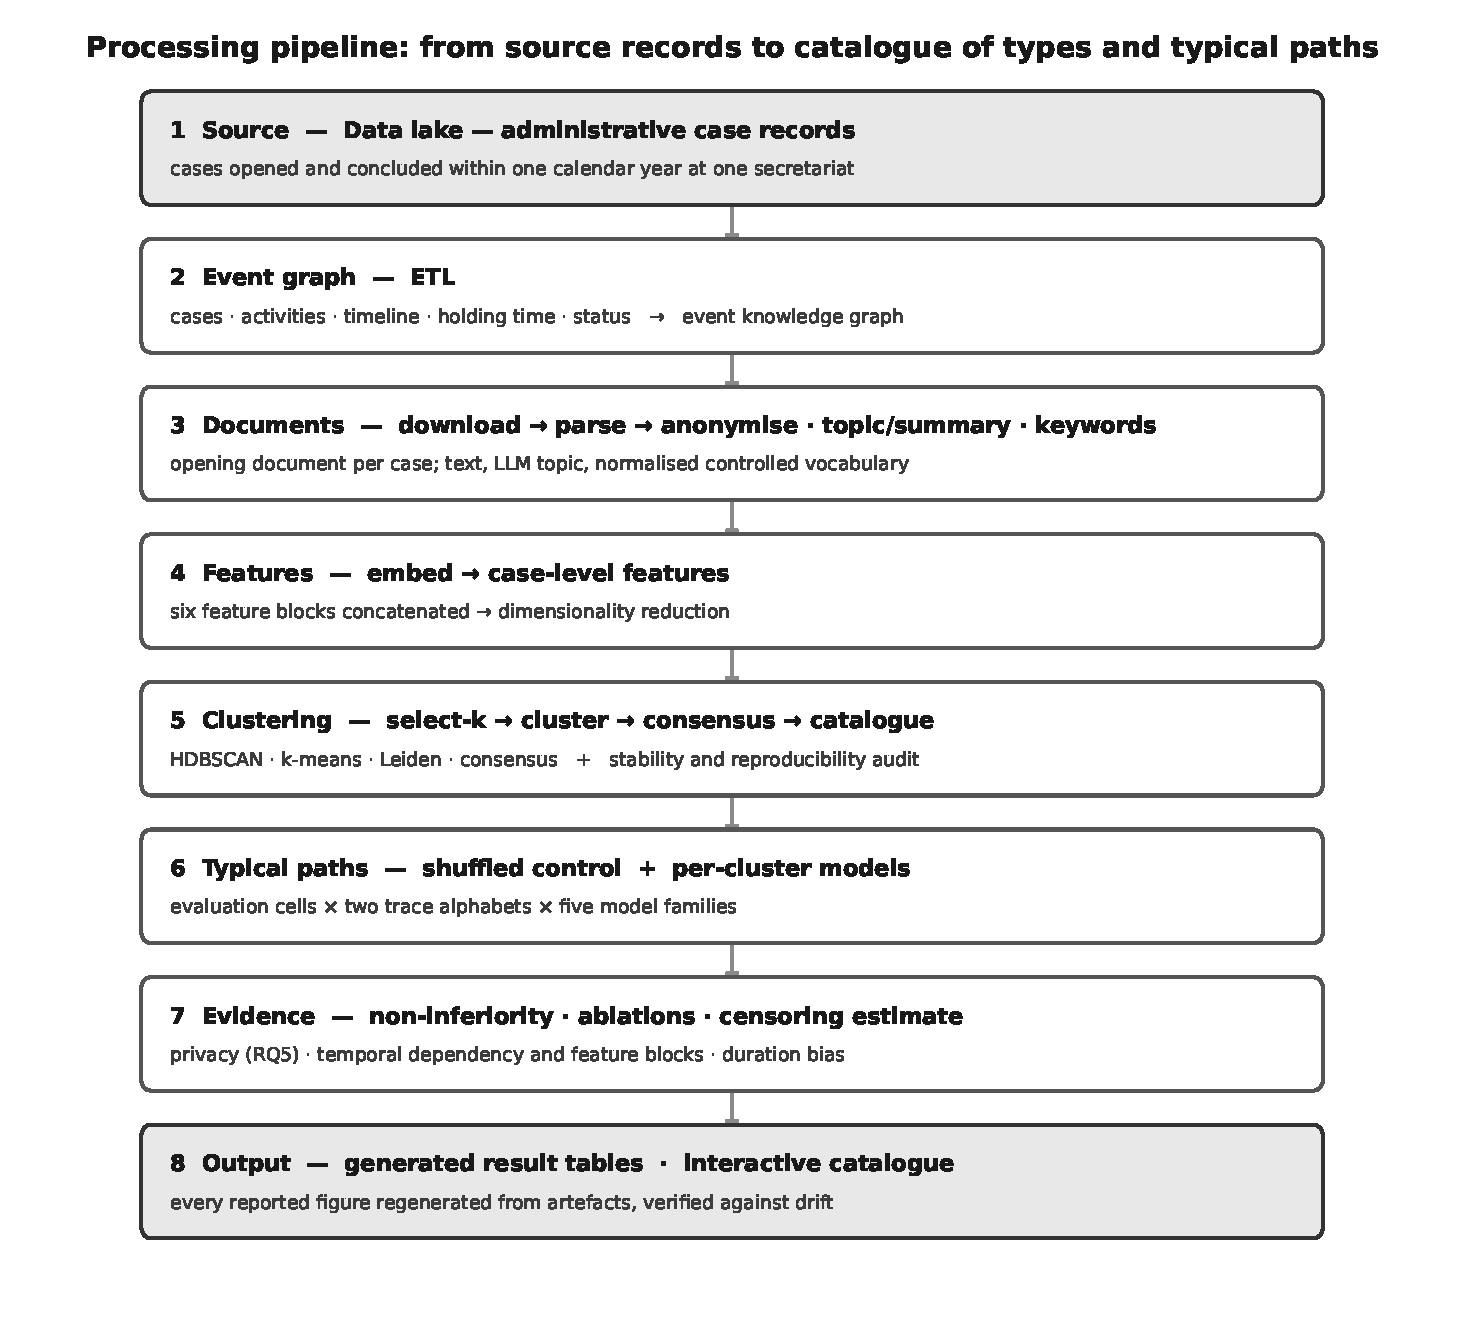
\includegraphics[width=0.86\textwidth]{pipeline-macro-en.pdf}
\caption{Pipeline from source event log to catalogue and generated evidence tables.}
\label{fig:pipeline}
\end{figure}

\paragraph{Controls.}
The shuffled-partition control is generated by permuting the labels of a real clustering, which
preserves cluster count, size distribution and the population that survives the evaluation
floor, so the only difference from the real partition is membership. The list of control cells
is derived from the list of real cells by the stage that runs them, rather than written
alongside it, so the two cannot diverge without failing.

\paragraph{The evidence layer.}
The stages above produce the artefact; the ones that follow exist to try to knock it down, and
each answers an objection a sceptical reader would be right to raise. All of them run per
alphabet wherever the quantity they measure depends on the alphabet.

\begin{itemize}
  \item \textbf{Block and history ablation} --- \emph{is it the documentary content that groups,
    or would anything group?} Feature blocks are zeroed one at a time and each case's history is
    truncated, measuring how far the partition moves.
  \item \textbf{Corpus bias} --- \emph{do the cases that conclude within the year represent the
    cases opened in it?} Right-censoring is estimated month by month (Section~\ref{sec:bias})
    rather than assumed benign.
  \item \textbf{Temporal holdout} --- \emph{does the advantage survive when the partition sees
    only part of each case's history?} The cuts are rescored over the cases all of them evaluate,
    since otherwise different populations would be compared.
  \item \textbf{Non-inferiority} --- \emph{does suppressing personal data cost utility, against a
    margin fixed before measuring?}
  \item \textbf{Constraint cost} --- \emph{what does the validity guarantee charge the
    generator?}
  \item \textbf{Conformance} --- \emph{how much of the observed behaviour does the discovered
    model reproduce, and how much more does it permit?}
  \item \textbf{Stability} --- \emph{does the partition survive resampling of its own members?}
  \item \textbf{Refit audit} --- \emph{does each stored clustering reproduce from the feature
    matrix it declares?}
  \item \textbf{Control partition} --- introduced in Section~\ref{sec:controls} and formalised in
    Section~\ref{sec:estimand}, the one that decides whether any of the others has anything to
    act on.
\end{itemize}

One lesson, methodological before it is empirical, organises the whole layer: \textbf{the
comparator decides the answer}. The same models, over the same cases, support different claims
according to what they are measured against --- which is why this study fixes its estimand before
measuring and reports the comparator beside every number.

\paragraph{Choosing among admitted partitions.}
$\Delta^{*}$ decides which partitions enter the study but does not order them
(Section~\ref{sec:estimand}). To choose among the admitted ones we use an explicit score with
three terms and weights declared in advance: \textbf{downstream performance}, weight 0.5,
measured over the \emph{common set} --- the cases that \emph{every} partition evaluates, without
which performance would be compared over different populations --- and scaled from the floor the
best shuffled partition reaches; \textbf{coverage}, weight 0.3, the fraction of the corpus that
survives the 30-trace floor; and \textbf{internal quality}, weight 0.2, the mean of two rescaled
validity indices. The weights are a choice, so the decision is put through a sensitivity sweep
over five weighting schemes --- balanced, downstream-first, coverage-first, quality-first and
equal thirds --- reporting the winner under each. A choice that survives only one weighting is a
choice of the weighting.

\paragraph{Reproducibility.}
Feature matrices are stamped with a digest of their inputs, and the clustering and evaluation
stages refuse to run against features whose stamp does not match the arm they claim --- a guard
rather than a convention. An audit stage refits each stored clustering from its own stamped
matrix, replays the recipe that clustering declares, including the noise policy of
Section~\ref{sec:noise}, and compares the result to the stored labels; its outcome is reported in
Section~\ref{sec:res-rq1}. A second audit walks the whole artefact tree and checks that every
file still declares the stage that produced it and that the declared inputs still digest the same
way. That chain --- question, version, inputs, refit --- is what turns ``this was run'' into
``anyone can re-run this''.

Document and topic embeddings are cached on disk, so switching arms restores identical vectors
rather than recomputing them; we verified that a raw--anonymised--raw cycle leaves the feature
matrix unchanged. A document whose anonymised text is byte-identical to its raw text keeps the
vector it already has rather than being reprocessed. It is not excluded, but it contributes no
anonymisation signal either, and the stage records how many documents are in that condition.

\paragraph{From artefacts to this paper.}
Every quantitative table in this paper is generated from stored artefacts by a single pipeline
stage, which also regenerates the corresponding tables in the project's internal results
document. A verification mode re-renders both the manuscript's tables and the internal
document's and fails if either has drifted from the artefacts, so a figure cannot be edited into
a table without the underlying evidence changing first. The complete grid of parameter
combinations is not printed here; it is regenerable from the stored artefacts.

Generated tables are the easy half. The numbers a reader actually encounters are in prose, and
prose is hand-written; a regeneration check cannot see it. We therefore maintain a second check,
run with the test suite, that holds an explicit register of the load-bearing quantitative claims
in the running text, resolves each to its path in the artefact tree, and fails in either
direction --- if a figure in the prose no longer rounds to the artefact it cites, or if the
artefact changes and the sentence is not updated with it. The register includes sign assertions,
so a rewording that preserves a magnitude while erasing the sign of a result also fails. It is
not exhaustive, and we make the narrower claim it supports: the figures it covers cannot drift
silently, and any figure not in it is verified only by reading.

\paragraph{Statistical procedures.}
The comparison between the raw and anonymised arms uses a paired bootstrap over the cases both
arms evaluate, with 2{,}000 replicates, conducted per alphabet and never across alphabets. The
pair is the case rather than the cell, which removes from the interval the variation due to case
difficulty. A conclusion of non-inferiority requires the one-sided 90\% lower bound of the
difference to clear a margin of 0.01 accuracy points, registered before the data existed, and a
sensitivity margin of 0.005 is reported alongside so that the conclusion's robustness to the
choice of margin is visible rather than assumed.

The relationship between a partition's internal quality and its downstream quality is tested by
rank correlation under a Monte Carlo permutation test with 20{,}000 draws, over the fourteen real
parameterisations of a single alphabet. Eight quantities are tested: four internal validity
indices --- DBCV, silhouette, Davies--Bouldin and Calinski--Harabasz --- and four descriptors of
partition shape --- cluster count, median cluster size, final noise rate, and the fraction density
would refuse before the assignment of Section~\ref{sec:noise}. All are tested without correction
for multiplicity, and all require the indices to come from one \emph{metric space}: indices
computed in different spaces are not comparable and cannot be pooled into a single correlation, so
the procedure aborts rather than silently aggregate a partition from outside the common space.

That design has low power, and the power is a property of the design rather than of the outcome:
with fourteen observations at $\alpha = 0.05$ the test rejects only for $|\rho| \geq 0.534$, and
attains 80\% power only near $|\rho| = 0.75$. The statement rule is therefore fixed before the
result is known: absent rejection we report absence of evidence and make no equivalence claim
about the indices, because the procedure alone establishes neither.

\section{Results}\label{sec:results}

\subsection{A catalogue the declared taxonomy does not supply (RQ1)}\label{sec:res-rq1}

Clustering the 5{,}243 cases yields between 40 and 120 types across the sixteen configurations,
with no singleton clusters under any of them. On the raw arm, density-based clustering produces
64 types with a median size of 50 cases and 879 cases left unassigned; centroid clustering
produces 64 types with a median size of 70 and no unassigned cases; consensus produces 120 types
with a median size of 33. Cluster-wise stability, assessed by drawing 25 subsamples of 80\% of
the cases, refitting, and matching each original cluster to its best Jaccard overlap
\citep{hennig2007stability}, gives a mean recovery of 0.7526 on the raw arm and 0.7724 on the
anonymised arm, with 47 of 64 and 47 of 61 types recovered above 0.60. Two limits attach to that
figure. It is a lower bound, because the clusterer is refit on each subsample but the
dimensionality reduction is not; and it was computed for the two density-based clusterings only,
so the remaining fourteen carry no stability estimate.

Against the administration's own taxonomy, the emergent partitions agree moderately, and the
level depends on which clustering is used. Across the eight main clusterings, ARI ranges from
0.086 to 0.202 and purity from 0.732 to 0.759. The majority-class baseline differs by scope and
both are reported: 0.302 for the six clusterings scored on all 5{,}243 cases, and 0.276 for the
two density-based ones, which are scored only on the cases they assign (4{,}364 and 4{,}504 of
5{,}243, the remainder being unassigned as noise). The upper end of the ARI range belongs to the
density-based clusterings; the algorithms that assign every case reach ARI 0.086 to 0.129. The
population confound identified in Section~\ref{sec:res-rq2} applies here as well, and we report
both rather than quoting the flattered figure alone.

The result that does not depend on that choice is what happens when one label is removed. A
single catch-all --- covering official documents of every kind, and applied to 30.5\% of the
5{,}445 concluded cases and 30.2\% of the 5{,}243 analysed --- accounts for most of the
disagreement. Excluding it, ARI rises to 0.352 for the density clusterings and to 0.166--0.256
for the full-coverage ones: a relative increase of 74\% to 110\%, in every case.

That increase needs a null before it can carry the reading we give it, because removing any
large class changes the index. Table~\ref{tab:catch-all-null} supplies one: for each clustering
we drop a randomly chosen set of whole declared classes totalling within 10\% of the catch-all's
size, and rescore. Removing random classes of that size \emph{lowers} agreement --- null means
of 0.064 to 0.160 against unrestricted ARI of 0.086 to 0.202 --- while removing the catch-all
raises it to 0.166--0.352. Across eight clusterings and roughly seven hundred draws each,
\textbf{no null draw reaches the observed value}, at $z$ between 7.3 and 17.2.

That null has a limitation we should name rather than let a reader discover. The catch-all holds
1{,}663 cases and no other declared class exceeds 764, so a size-matched draw is necessarily a
\emph{union} of many classes --- a median of twenty-seven. The comparison it makes is therefore
between removing one large heterogeneous class and removing many small ones, which is not
cleanly a test of \emph{which} class was removed.

The contrast that does isolate that is simpler, and it is unanimous. Dropping each of the three
next-largest declared classes on its own \emph{lowers} agreement in every case --- 24 of 24
single-class drops across the eight clusterings --- while dropping the catch-all raises it in
8 of 8. On the raw-arm centroid clustering, agreement is 0.128 unrestricted, 0.246 without the
catch-all, and 0.107, 0.122 and 0.118 without each of the next three classes in turn. Removing a
large class is not what produces the effect, and removing a large class is in fact mildly
harmful; removing \emph{this} class is what produces it.

The declared taxonomy is therefore not uninformative. It degrades concentrated in one class,
which is what a filing classification does when it is maintained for routing paperwork rather
than for describing procedure. The reading that class is a defect of the taxonomy is ours and
should be resisted: a classification maintained to route documents is fit for the purpose it
serves, and we are scoring it against an analytical purpose it was never designed for.

%% GENERATED by `pipeline run results` - do not edit by hand.
\begin{table}[htbp]
\centering
\caption{The catch-all class against a same-size random-class null.}\label{tab:catch-all-null}
\begin{tabular}{lrrrrrr}
\toprule
clustering & ARI all & ARI excl. & null mean & null max & $\geq$ obs. & $z$ \\
\midrule
exp-raw/hdbscan & 0.1383 & 0.2767 & 0.1010 $\pm$ 0.0189 & 0.1311 & 0/724 & 9.3 \\
exp-raw/kmeans & 0.1324 & 0.2548 & 0.0988 $\pm$ 0.0106 & 0.1231 & 0/724 & 14.8 \\
exp-raw/leiden & 0.1197 & 0.2348 & 0.0885 $\pm$ 0.0102 & 0.1076 & 0/724 & 14.3 \\
exp-anon/hdbscan & 0.1450 & 0.2831 & 0.1072 $\pm$ 0.0187 & 0.1375 & 0/724 & 9.4 \\
exp-anon/kmeans & 0.1317 & 0.2585 & 0.0974 $\pm$ 0.0110 & 0.1225 & 0/724 & 14.6 \\
exp-anon/leiden & 0.1161 & 0.2303 & 0.0851 $\pm$ 0.0102 & 0.1068 & 0/724 & 14.2 \\
\bottomrule
\end{tabular}
\par\vspace{2pt}\footnotesize\raggedright Null: drop a randomly chosen set of whole declared classes totalling within 10\% of the catch-all's size, and rescore. Removing random classes of the same size lowers agreement; removing the catch-all raises it. No null draw reaches the observed value for any clustering.
\end{table}


\subsubsection{What an entry looks like}

An artefact offered as a transparency instrument should be shown, not only measured.
Table~\ref{tab:catalogue} gives ten entries from the partition Section~\ref{sec:selection}
selects as the deliverable --- the six largest evaluated types and the four smallest --- with
the generated name, the number of cases assigned, and the support measures for that type's own
typical path. Names are reproduced as the pipeline produced them, and are unvalidated
(Section~\ref{sec:naming}).

The table is included because the averages elsewhere in this section conceal how unevenly
evidenced the entries are, and a reader deciding whether to trust the artefact needs to see the
spread rather than the mean. The best entries are very good: a company-registration type over
325 cases reaches 0.974 next-step accuracy with complete unit recall over a four-visit path and
no fabricated transitions. Others are weak in ways a published catalogue would have to disclose.
A leave-and-indemnity type over 261 cases reaches 0.522 with unit recall 0.515, and a ponto-justification type over 137 cases reaches 0.424 --- both summarising in three or four
visits a set of cases that evidently do more than that. A property-rental payment type covers
296 cases with a 28-visit path that recovers 0.917 of what its cases do and is the only entry in
the sample that fabricates at all.

Two things follow for anyone publishing such a catalogue. An entry is not a uniform object, so
case counts and support measures belong beside every published type rather than in an appendix.
And the weak entries are not the small ones --- three of the four weakest here have more than
130 cases each --- so size alone is not a usable proxy for whether an entry can be trusted.

%% GENERATED by `pipeline run results` - do not edit by hand.
\begin{table}[htbp]
\centering
\caption{Illustrative catalogue entries, largest and smallest evaluated types.}\label{tab:catalogue}
\footnotesize
\begin{tabular}{p{0.42\textwidth}rrrr}
\toprule
process type (generated name) & cases & eval. & top-1 & unit rec. \\
\midrule
Gestão de Contracheques e Solicitações de Pagamentos Indenizatórios & 318 & 312 & 0.850 & 0.978 \\
Solicitação de Autorização para Adesão a Ata de Registro de Preços & 229 & 217 & 0.733 & 0.823 \\
Registro de Alterações Contratuais e Consolidação Societária de Empresas & 210 & 210 & 0.984 & 1.000 \\
Solicitação de Pagamento de Serviços de Mão de Obra Terceirizada & 198 & 198 & 0.771 & 0.924 \\
Retirada de Descontos Indevidos em Contracheques de Servidores & 188 & 188 & 0.770 & 0.916 \\
Gestão de Pessoal e Contratações Temporárias & 192 & 185 & 0.718 & 0.658 \\
Justificativa e Abono de Faltas por Doença ou Trabalho Remoto & 42 & 39 & 0.547 & 0.810 \\
Autorização de Recebimento de Bens Arrematados em Leilão & 38 & 35 & 0.640 & 0.816 \\
Solicitação de Pagamento de Fornecimento de Água Tratada & 31 & 31 & 0.785 & 0.977 \\
Solicitação de Abono de Faltas e Justificativa de Ponto & 30 & 30 & 0.570 & 0.857 \\
\bottomrule
\end{tabular}
\par\vspace{2pt}\footnotesize\raggedright Illustrative entries from the catalogue, largest and smallest evaluated types. Names are generated (Section 4.7) and unvalidated; measures are for the GRU path on the routing alphabet, the family that gains most on routing (Section 4.8).
\end{table}


We do not claim the emergent catalogue is correct. There is no ground truth against which it
could be scored --- the absence of a trustworthy classification is the premise of the work.
What can be established is that it is not arbitrary (Section~\ref{sec:res-rq3}) and that it is
reproducible: all nineteen clusterings defined as a function of the feature matrix refit exactly
from their stamped inputs (the two consensus partitions are derived from other labels, not from
features, and are outside that check).

%% GENERATED by `pipeline run results` - do not edit by hand.
\begin{table}[htbp]
\centering
\caption{Agreement between the emergent partition and the declared taxonomy.}\label{tab:taxonomy}
\footnotesize
\begin{tabular}{llrrrrr}
\toprule
clustering & scope & $n$ & majority & purity & NMI & ARI \\
\midrule
exp-anon/hdbscan & all & 5,243 & 0.302 & 0.730 & 0.530 & 0.145 \\
exp-anon/hdbscan & excl.\ catch-all & 3,660 & 0.208 & 0.775 & 0.621 & 0.283 \\
exp-anon/kmeans & all & 5,243 & 0.302 & 0.735 & 0.531 & 0.132 \\
exp-anon/kmeans & excl.\ catch-all & 3,660 & 0.208 & 0.784 & 0.624 & 0.259 \\
exp-anon/leiden & all & 5,243 & 0.302 & 0.727 & 0.521 & 0.116 \\
exp-anon/leiden & excl.\ catch-all & 3,660 & 0.208 & 0.776 & 0.613 & 0.230 \\
exp-raw/hdbscan & all & 5,243 & 0.302 & 0.728 & 0.527 & 0.138 \\
exp-raw/hdbscan & excl.\ catch-all & 3,660 & 0.208 & 0.775 & 0.621 & 0.277 \\
exp-raw/kmeans & all & 5,243 & 0.302 & 0.738 & 0.531 & 0.132 \\
exp-raw/kmeans & excl.\ catch-all & 3,660 & 0.208 & 0.784 & 0.622 & 0.255 \\
exp-raw/leiden & all & 5,243 & 0.302 & 0.723 & 0.524 & 0.120 \\
exp-raw/leiden & excl.\ catch-all & 3,660 & 0.208 & 0.780 & 0.618 & 0.235 \\
\bottomrule
\end{tabular}
\end{table}


\subsection{Feature blocks and temporal dependency}\label{sec:res-ablation}

Cases are clustered from their complete activity history. This is a design choice rather than an
oversight: the catalogue is a retrospective account, and because the study declines to rely on
the declared type, the partition must use whatever signal the record affords. The ablation in
Table~\ref{tab:ablation} asks a different question --- when does that signal become available?

Removing the keyword block perturbs the partition about as much as discarding half of every
case's history (ARI 0.414 against 0.430), so the controlled vocabulary contributes signal the
other blocks do not carry. Removing the topic block costs less (0.577), which is expected: topic
and semantic representations are both derived from the same opening document.

Truncating each case's features at 75\%, 50\% and 25\% of its own timeline degrades agreement
with the full-history partition smoothly --- ARI 0.581, 0.430 and 0.296 --- rather than
collapsing. A partition built from partial histories is still substantially the same partition,
but a real share of the evidence arrives late. Read as a statement about administrative work
rather than about method, this says that what a case \emph{is} becomes progressively clearer as
it runs: routing history and accumulated actions carry type information that the opening
document does not fully determine.

Two consequences follow, both of them scope statements. The catalogue is retrospective by
construction, which is what an as-is instrument should be. And assigning a type at intake is a
distinct and harder problem: at a 25\% cutoff the partition retains ARI 0.296 against the
full-history one, informative but far from equivalent. Doing that well would require richer
early-stage features than the single opening document embedded here.

\subsubsection{Does the partition predict the future because it has seen it?}\label{sec:holdout}

Clustering on complete histories raises a sharper objection than scope, and it bears directly on
RQ3 rather than on RQ1. Two of the six feature blocks are built from the organisational units a
case visits and the transitions between them, so on the routing alphabet a held-out case is
assigned to a cluster partly by the very sequence the model is then asked to predict. If that is
what produces the routing gain, the gain measures circularity rather than process structure.
Held-out splitting does not address this, because the leak is inside the feature construction
rather than across the split.

The ablation clusterings make the objection partly testable. Each truncated variant builds its
features from the first fraction of every case's own timeline; we then predict on the \emph{full}
held-out traces. The test is weaker than it first appears and we state its limit before its
result: truncating at 25\% still lets the unit blocks see the first quarter of the sequence the
model is scored on from step one, so the leak is reduced rather than removed. What the
comparison can show is whether the gain depends on the \emph{later} part of the history, not
whether it is free of the earlier part.

It does not, and the naive reading of the gradient is wrong in a way worth reporting. Scored as
each truncation was evaluated, the routing gain falls from 0.0381 on full histories to 0.0145 at
25\%. But those four rows are computed on four different populations --- 962, 946, 897 and 889
held-out cases --- and the fall is almost entirely the baseline moving, not the partition losing
information. Per-cluster accuracy is flat across the four truncations (0.6576 to 0.6572, a
change of 0.0004), while the global model \emph{rises} from 0.6195 to 0.6427. A single global
chain cannot change with the clustering, so that rise is the evaluated population becoming
easier as truncation shrinks it.

Rescoring every truncation on the 637 cases all four evaluate --- the same correction this
section applies to the algorithm comparison --- gives gains of 0.0380, 0.0400, 0.0289 and
0.0310. Roughly \textbf{82\% of the routing gain survives when the partition is built from the
first quarter of each case}, and the residual gradient is not monotone: the 25\% truncation
scores above the 50\% one. The action gain stays near zero throughout, consistent with
Section~\ref{sec:res-rq3}.

Three limits bound what this establishes. The truncation is partial, as stated above. The
matched population is the easier subset that survives every truncation, so it is not the corpus.
And the test runs on one arm and one algorithm. Our conclusion is correspondingly narrow: the
routing result is not primarily an artefact of clustering on the later history, and we cannot
show it is free of the early history at all.

%% GENERATED by `pipeline run results` - do not edit by hand.
\begin{table}[htbp]
\centering
\caption{Downstream gain when the partition sees only part of each case's history.}\label{tab:temporal-holdout}
\begin{tabular}{lrrrrr}
\toprule
clustering features & clusters & per-cluster & global & gain (as evaluated) & gain (matched) \\
\midrule
full history & 41 & 0.6937 & 0.6856 & 0.0081 & \textbf{0.0097} \\
first 75\% & 44 & 0.6942 & 0.6893 & 0.0049 & \textbf{0.0063} \\
first 50\% & 46 & 0.6937 & 0.6940 & -0.0003 & \textbf{0.0040} \\
first 25\% & 32 & 0.6777 & 0.6924 & -0.0147 & \textbf{-0.0057} \\
\bottomrule
\end{tabular}
\par\vspace{2pt}\footnotesize\raggedright Each row clusters on features truncated at a fraction of every case's own timeline, then predicts on the full held-out traces. The unmatched rows evaluate different populations, so their gradient mostly reflects the global baseline moving; the matched block rescores every truncation on the cases all four evaluate. The final column rescores every truncation on the 1,091 cases all four evaluate, which is the comparison the unmatched column cannot make.
\end{table}


%% GENERATED by `pipeline run results` - do not edit by hand.
\begin{table}[htbp]
\centering
\caption{Feature-block and temporal-dependency ablations.}\label{tab:ablation}
\begin{tabular}{lrrr}
\toprule
variant & ARI & NMI & clusters \\
\midrule
History truncated at 75\% & 0.798 & 0.895 & 68 \\
History truncated at 50\% & 0.649 & 0.816 & 70 \\
History truncated at 25\% & 0.467 & 0.717 & 53 \\
Keyword block removed & 0.596 & 0.838 & 65 \\
Topic block removed & 0.840 & 0.905 & 71 \\
\bottomrule
\end{tabular}
\par\vspace{2pt}\footnotesize\raggedright Each variant rebuilds the features under one change and re-clusters; agreement is measured against the full-history partition (64 clusters over 5,243 cases).
\end{table}


\subsection{What separates one partition from another, and what does not (RQ2)}\label{sec:res-rq2}

\subsubsection{Three distinct discards, and why raw comparison is invalid}

Coverage is lost three times, and conflating them produces the wrong conclusion. Density-based
clustering leaves 739 to 879 cases unassigned; centroid, modularity and consensus clustering
assign every case. Separately, the requirement of at least 30 traces per cluster removes
clusters from evaluation for every algorithm equally. And on the routing alphabet only, a case
whose itinerary contains fewer than two organisational units carries no transition to predict
and is dropped before either of the other two applies: \textbf{1{,}082 of the 5{,}243 cases,
20.6\%}, never enter that arm at all.

That third discard is alphabet-specific and it is the reason the two arms are not scored on the
same population --- the action alphabet is evaluated over all 5{,}243 cases, the routing
alphabet over 4{,}161. It also reapportions the loss the floor appears to cause. On the routing
alphabet, of the 1{,}187 to 2{,}207 cases absent from evaluation, roughly 1{,}082 are
single-unit cases rather than casualties of the floor, which leaves 58--77\% of the corpus
evaluated; consensus discards nothing at clustering time yet evaluates only about 60\%, because
fragmenting into 120 clusters puts many of them below the floor, while centroid clustering
reaches 77\%. On the action alphabet the floor removes only 105 to 1{,}156 cases and coverage
runs 77--98\%, so for most action-alphabet cells the floor costs \emph{less} than density
clustering's noise rather than more.

Because density-based clustering is scored only on the cases it chose to keep, comparing raw
per-algorithm numbers compares different populations. Rescoring every clustering on the 824
cases that all sixteen evaluate removes the confound without re-running anything, since
per-case correctness is stored alongside the held-out identifiers.

One property of that rescoring must be stated, because Section~\ref{sec:res-rq3} makes a great
deal of the same issue. The per-case record used here is the one belonging to whichever of the
five model families scored highest in that cluster, selected on the held-out data it is then
scored on. Every common-set figure in this subsection is therefore a per-cluster best-of-five,
and is an upper bound in the same sense as the selected-best figures of
Section~\ref{sec:res-rq3}. It is applied identically to all sixteen clusterings, so it does not
bias the comparison \emph{between} them, which is what this subsection uses it for; it would
bias any reading of the absolute level, and we do not offer one.

The apparent advantage disappears. On its own evaluated set the raw-arm density clustering
scores 0.6891, the best of the sixteen; on the common set it scores 0.6908, second-worst, with
only the coarse-parameter density clustering of the same arm below it. Every other clustering
gains between 0.020 and 0.033 under the restriction, because the restriction removes the
difficult cases that clustering had already discarded, while it gains 0.002 --- its own set was
already the easier subset.

The mechanism is narrower than ``density-based clustering'' as a family. Of the four density
clusterings, only the raw-arm one at 16.8\% noise shows the near-zero gain; the other three gain
0.020 to 0.023, indistinguishable from the partitional methods. What produces the reversal is a
high discard rate, not the algorithm family. Across all sixteen the spread on the common set is \textbf{0.008}.

Two qualifications bound what that number can be made to say. First, the comparison is made on
the cases every algorithm can model, which by the analysis in the next paragraph are the easier
ones --- restricting to the intersection removes precisely the cases on which the algorithms
might have differed, so this is a statement about the shared population, not about the corpus.

Second, and more restrictive, a small spread is not by itself evidence of equivalence, and this
study cannot convert it into one. A case-level bootstrap over the 824 common cases, 2{,}000
replicates, puts the spread at 0.0079 with a 95\% interval of $[0.0064, 0.0139]$ and a one-sided
90\% upper bound of 0.0124. An equivalence claim requires the bound, not the point estimate, to
fall inside a margin. Against the only margin this study registered --- 0.01 absolute top-1, and
registered for the anonymisation comparison on the action alphabet rather than for a sixteen-way
range on the routing one --- the bound does not fall inside it. We therefore report the spread
descriptively and make no equivalence claim: on the cases all algorithms can model, the observed
differences between clusterings are small, and this design cannot establish that they are
immaterial. Doing so would need a margin specified for this comparison and enough common cases
to tighten the interval, which is the same standard we hold the anonymisation result to in
Section~\ref{sec:res-rq5}.

That the discarded cases are harder, rather than unmodellable, can be checked directly. The
algorithms that assign every case score 0.556--0.585 on the cases density clustering rejects,
against 0.675--0.692 on the rest: a gap of roughly 0.10 to 0.14, or 14--20\% relatively worse.
For an artefact intended to describe an administration's actual work, silently omitting 14--17\%
of it is a real cost that buys no accuracy, and the discard should be read as a limitation of
that algorithm rather than as evidence of its quality.

%% GENERATED by `pipeline run results` - do not edit by hand.
\begin{table}[htbp]
\centering
\caption{Clustering comparison on a common set of cases.}\label{tab:common-set}
\footnotesize
\begin{tabular}{lrrrr}
\toprule
clustering & own $n$ & own set & common set & $\Delta$ \\
\midrule
exp-raw/leiden & 1,153 & 0.7107 & \textbf{0.7129} & 0.0022 \\
exp-raw-ksil/kmeans & 1,195 & 0.7081 & \textbf{0.7127} & 0.0046 \\
exp-anon/leiden & 1,122 & 0.7096 & \textbf{0.7114} & 0.0018 \\
exp-raw-kelbow/kmeans & 1,169 & 0.7126 & \textbf{0.7111} & -0.0015 \\
exp-raw-hcoarse/hdbscan & 1,207 & 0.7070 & \textbf{0.7109} & 0.0039 \\
exp-anon/hdbscan & 1,183 & 0.7054 & \textbf{0.7107} & 0.0053 \\
exp-anon-hcoarse/hdbscan & 1,199 & 0.7072 & \textbf{0.7101} & 0.0029 \\
exp-raw/hdbscan & 1,185 & 0.7030 & \textbf{0.7098} & 0.0068 \\
exp-anon/kmeans & 1,186 & 0.7058 & \textbf{0.7094} & 0.0036 \\
exp-raw-lres/leiden & 1,117 & 0.7046 & \textbf{0.7093} & 0.0047 \\
exp-anon-lres/leiden & 1,025 & 0.7049 & \textbf{0.7091} & 0.0042 \\
exp-raw/kmeans & 1,183 & 0.7067 & \textbf{0.7088} & 0.0021 \\
exp-anon-kelbow/kmeans & 1,170 & 0.7042 & \textbf{0.7074} & 0.0032 \\
exp-anon-ksil/kmeans & 1,195 & 0.7038 & \textbf{0.7074} & 0.0036 \\
\bottomrule
\end{tabular}
\par\vspace{2pt}\footnotesize\raggedright All clusterings rescored on the 967 cases every one of them evaluates. Spread on the common set: \textbf{0.0055}.
\end{table}


\subsubsection{Internal validity indices}

Table~\ref{tab:intrinsic} reports each index against downstream quality across the sixteen
clusterings. Both results in this subsection --- the index correlations and the common-set
comparison above --- are computed on the routing alphabet, and we state them as such rather than
as general claims about clustering. All sixteen indices are computed in the same space, the
reduced embedding in which clustering is performed. This is not automatic: the two consensus
partitions are derived from the other algorithms' label assignments rather than from the feature
matrix, and indices computed in that co-association representation are not on the same scale as
the rest --- a one-hot encoding of agreement makes members of a consensus cluster nearly
coincident, which inflates every compactness measure. We therefore recompute the consensus
partitions' indices in the shared embedding, and the evidence pipeline refuses to pool indices
carrying different space stamps.

Taken at face value the correlations are moderate and point the way the indices intend:
$\rho = 0.36$ for DBCV, $0.35$ for silhouette, $-0.48$ for Davies--Bouldin. None is significant
--- a permutation test over 20{,}000 draws rejects nothing, the smallest $p$ being 0.059 --- and
at sixteen observations the design rejects only for $|\rho| \geq 0.497$, so associations of the
size observed are exactly the ones it cannot resolve. Read no further and the result is an
underpowered null.

Reading further is what the data reward, because the association that does exist is not with
utility. Table~\ref{tab:index-mechanism} traces it. Across all sixteen clusterings, silhouette
is strongly related to \emph{how much a partition throws away}: $\rho = 0.61$ with the share of
cases discarded as noise. Discarding raises the score on the partition's own evaluated set
($\rho = 0.68$), because the cases a density method declines to assign are the hard ones
(Section~\ref{sec:res-rq2}). An index that rewards discarding, scored against a metric computed
on what survives the discarding, will correlate with it for reasons that have nothing to do with
cluster quality.

Restricting to the twelve clusterings that assign every case closes that channel by
construction, and one relationship in that subset is strong enough to survive the scrutiny a
sample of twelve deserves. Silhouette tracks granularity almost deterministically:
$\rho = 0.87$ with median cluster size and $-0.84$ with the number of clusters, and the
association holds on every subset we can form --- dropping the consensus partitions gives 0.92,
dropping the modularity ones 0.93, and the six centroid clusterings alone 0.83. On this corpus,
what silhouette measures is how coarse the partition is.

That finding is conditional on how the twelve were produced, and the condition is not incidental.
They are six centroid clusterings at different $k$, four modularity clusterings at different
resolutions, and two consensus partitions at a fixed $k$ --- so granularity is the variable the
parameter sweep deliberately manipulates. Finding that a compactness index tracks the knob the
sweep turns is closer to a property of that design than to a discovery about the corpus, and on
the six configuration-level points the association is $\rho = 0.77$ at $p = 0.10$ under an exact
permutation test over all orderings, which does not clear significance. What we can say is that on partitions generated this
way the index is a granularity measure; whether it would separate partitions of equal
granularity is a question this design cannot pose.

Two things that look like further findings are not, and we set them aside rather than count
them. Silhouette also correlates with coverage at $\rho = 0.84$, but coverage is determined by
how many clusters clear a size floor, so this is a restatement of the granularity result rather
than an addition to it: controlling for median cluster size, the partial correlation between
silhouette and coverage is 0.125. And silhouette correlates with accuracy at
$\rho = 0.35$ against $\rho = 0.84$ for coverage, which invites the reading that it predicts one
and not the other --- but twelve clusterings are six raw/anonymised pairs, and a bootstrap that
resamples configurations rather than clusterings puts the difference between those two
correlations at $[-0.02, +0.99]$ over 5{,}000 draws. The interval includes zero. We cannot distinguish them.

The same discipline applies to the null. At twelve observations the design resolves only
$|\rho| \geq 0.58$, so $\rho = 0.35$ is not evidence of a weak association any more than it is
evidence of a strong one; it is the range this design cannot see into. Stratifying by cluster
size leaves the parent partition's silhouette with no association with accuracy in any band
($-0.10$, $-0.01$, $-0.12$), but silhouette is a partition-level constant, so those bands
contain twelve distinct values rather than 488 independent ones, and the bands do not fully hold
size fixed --- cluster size still predicts accuracy within the smallest and largest of them.

What RQ2 supports is therefore one positive finding and one unchanged negative. The positive
finding is that on this corpus these indices are substantially a measure of granularity, which
is a real property and not the one they are usually invoked for. The negative finding is the
same as before: no evidence that they predict downstream utility, at a design that could not
have detected a moderate association had one existed. We do not claim to have shown they fail to
predict it. The practical consequence follows from the positive half alone --- selecting a
clustering on silhouette here selects, in substance, for coarseness, and
Section~\ref{sec:selection} therefore selects on the quantities directly.

%% GENERATED by `pipeline run results` - do not edit by hand.
\begin{table}[htbp]
\centering
\caption{What the validity indices actually track.}\label{tab:index-mechanism}
\footnotesize
\begin{tabular}{lll}
\toprule
relation & population & $\rho$ \\
\midrule
Silhouette vs.\ share of cases discarded as noise & all 14 & -0.308 \\
Share discarded vs.\ accuracy on the partition's own set & all 14 & -0.204 \\
Silhouette vs.\ median cluster size & full-cov.\ 14 & 0.427 \\
Silhouette vs.\ number of clusters & full-cov.\ 14 & -0.325 \\
Number of clusters vs.\ coverage & full-cov.\ 14 & -0.991 \\
Silhouette vs.\ coverage & full-cov.\ 14 & 0.341 \\
\textbf{Silhouette vs.\ common-set accuracy} & full-cov.\ 14 & \textbf{-0.392} \\
\textbf{DBCV vs.\ common-set accuracy} & full-cov.\ 14 & \textbf{-0.057} \\
Silhouette vs.\ accuracy, small clusters only (mean top-1 0.623) & 233 clusters, 14 values & -0.151 \\
Silhouette vs.\ accuracy, medium clusters only (mean top-1 0.655) & 267 clusters, 14 values & -0.009 \\
Silhouette vs.\ accuracy, large clusters only (mean top-1 0.781) & 89 clusters, 14 values & 0.074 \\
\bottomrule
\end{tabular}
\par\vspace{2pt}\footnotesize\raggedright Granularity is the relationship that survives scrutiny at this sample size. The coverage rows are largely a restatement of it (partial correlation given median cluster size is small), and the difference between the coverage and accuracy correlations is not resolvable here -- its bootstrap interval over configurations includes zero. The band rows carry only as many distinct silhouette values as there are partitions, not as many as there are clusters, so they are far weaker evidence than their cluster counts suggest.
\end{table}


This result concerns indices computed on a reduced embedding, which is where clustering is
performed; it is not a claim about the embedding itself. It also does not contradict work
certifying these indices against recovery of a known partition, since no known partition exists
here.

%% GENERATED by `pipeline run results` - do not edit by hand.
\begin{table}[htbp]
\centering
\caption{Internal validity indices against downstream utility.}\label{tab:intrinsic}
\begin{tabular}{lrr}
\toprule
index & $\rho$ & $p$ \\
\midrule
DBCV & 0.538 & 0.053 \\
Silhouette & -0.516 & 0.060 \\
Davies--Bouldin & 0.464 & 0.100 \\
Calinski--Harabasz & -0.270 & 0.354 \\
Noise ratio (refused) & -0.055 & 0.853 \\
Number of clusters & 0.501 & 0.073 \\
Median cluster size & -0.524 & 0.061 \\
\bottomrule
\end{tabular}
\par\vspace{2pt}\footnotesize\raggedright Spearman rank correlation with downstream quality across 14 clusterings; permutation test with 20,000 draws. The downstream measure spans 0.112 (34\% relative).
\end{table}


\subsection{Typical paths against three controls (RQ3)}\label{sec:res-rq3}

\subsubsection{The partition carries the signal}

Permuting cluster membership while preserving cluster count, size distribution and evaluated
population reduces best next-step accuracy from 0.726 to 0.494 on the action alphabet, and from
0.672 to 0.457 on the routing alphabet. Nothing about the \emph{shape} of a partition produces
23 points; only membership does. The same conclusion holds without any learned model: the
within-cluster most-frequent-successor lookup scores 0.643 on real clusters and 0.447 on
shuffled ones, which is evidence of coherence independent of the sequence models entirely.

\subsubsection{What per-cluster modelling adds, measured honestly}

Table~\ref{tab:controls} reports all three baselines, and the comparison must be made carefully,
because the obvious way to make it is wrong.

Taking the best of the five model families in each cluster gives 0.726 on actions and 0.672 on
routing, against 0.713 and 0.610 for a single global third-order Markov chain: apparent gains of
0.013 and 0.063. That comparison is not like-for-like. The clustered figure is a per-cluster
\emph{maximum} over five families, selected using held-out data, while the global baseline is
one fixed family. Part of the apparent gain is the selection, not the partitioning.

Matching the families removes it. A third-order Markov chain fitted per cluster, against the
same chain fitted globally, gains \textbf{0.004} on actions and \textbf{0.035} on routing.
Fixing any single family throughout rather than choosing per cluster gives at most 0.005 on
actions and 0.053 on routing. On actions a per-cluster LSTM is \emph{worse} than the global
model \((-0.004)\).

We report both: the selected-best figures because they are what a practitioner choosing freely
would obtain, and the family-matched figures because they are what the partition itself
contributes. The honest statement of the second is that \textbf{on the action alphabet,
partitioning contributes almost nothing} --- 0.004 against a baseline of 0.713.

This exposes a symmetry worth naming. The paper's own argument is that the conventional
within-cluster baseline inflates the apparent contribution of clustering roughly sixfold;
selecting the best of five families against a single-family baseline inflates it again, roughly
threefold on actions. The same discipline has to apply at both levels.

The gap between the two alphabets is the substantive finding, and it must be measured on one
population before it can be stated. As reported so far the two arms are scored on different
populations: the 1{,}082 single-unit cases that carry no itinerary are absent from the routing
arm by construction (Section~\ref{sec:res-rq2}). Those are the simplest cases in the corpus, so
excluding them from routing while retaining them in actions biases the comparison in the
direction that flatters routing, and a ratio computed across the two is not interpretable.

We therefore re-fitted the action-alphabet models on the 4{,}161 multi-unit cases, so that both
alphabets are scored over the identical 323 clusters and 27{,}795 traces.
Table~\ref{tab:shared-population} reports the result, and the correction does not weaken the
finding --- it inverts one half of it. On all cases, a per-cluster Markov chain beats a global
one on actions by 0.0032 over these eight clusterings, the same near-zero gain the full sixteen
put at 0.004. On the shared population it \emph{loses} to the global model by 0.0087, and it
does so in all eight clusterings individually, from $-0.0020$ to $-0.0133$. Routing on that same
population gains 0.0359.

The mechanism is visible in the same table. Removing the single-unit cases costs the global model
0.011 of accuracy and the per-cluster models 0.023 --- twice as much. The small positive gain
that per-cluster action models showed was drawn disproportionately from the easiest cases in the
corpus; on the cases that actually have a routing decision to make, partitioning does not help
action prediction, it hurts it.

The substantive claim is therefore signed rather than scaled: \textbf{on one population,
per-cluster modelling helps on routing and does not help on actions}. Both magnitudes depend on
a choice we must expose rather than bury, and we expose it for both rather than only where it
is convenient.

Aggregating per-cluster accuracies to a corpus figure requires a weight, and the two defensible
weights disagree. Weighting each cluster by its membership --- which asks how a randomly chosen
\emph{case} is served --- gives $+0.0032$ on actions over all cases, $-0.0087$ on actions over
the shared population, and $+0.0359$ on routing. Weighting by held-out prediction steps --- the
pooled accuracy over every prediction actually made --- gives $-0.0044$, $-0.0047$ and
$+0.0292$. Two things follow. On actions the second weighting removes the sign change entirely:
per-cluster modelling is slightly negative on both populations, and restricting the population
moves it by 0.0003 rather than by 0.012, so the apparent inversion is an artefact of the weight
and not a population effect. On routing the gain is real under both weights but 18\% smaller
under the second, so the headline figure is weight-dependent in the same way and to a
comparable degree.

What survives either choice is the contrast and its direction: routing gains something between
0.029 and 0.036, actions gain nothing and may lose a little. That is the finding; the third
decimal place is not.

Re-fitting every family on the restricted population shows this is not a property of the Markov
chain (Table~\ref{tab:families-shared}). Membership-weighted, all five are negative there. The
selected-best figure behaves the same way: the per-cluster maximum over five families gains
0.0116 over a global model on all cases and \textbf{0.0007} on the shared population --- and
that maximum is an oracle, chosen on the same held-out data it is scored on, so it is an upper
bound rather than an estimate. An oracle over five families barely reaching parity with one
pooled chain is the clearest statement of the result.

We do not report an interval on the action deficit, and it is small enough that one is needed
before any strong claim rests on it; what the evidence supports is a sign and a recommendation,
not a magnitude. Which unit handles a case next depends on the procedure; which action is recorded
largely follows conventions shared across procedures. For an instrument whose purpose is to show
how work moves through an administration, the routing representation is both the more
informative and the better supported.

Size changes the picture on actions and not on routing. On actions the selected-best gain over a
global model is 0.003, 0.010 and 0.024 for small, medium and large clusters; since the pooled
selected-best gain of 0.013 corresponds to a family-matched 0.004, the family-matched gain below
150 traces is indistinguishable from zero, and a per-cluster action model is not worth training
there. On routing it is 0.055, 0.072 and 0.052 ---
essentially size-independent, and worth training throughout. Fabrication follows the same
split: unseen transitions fall from 6.04 to 1.10 with size on actions, but are already low on
routing and reach 0.038 on large clusters, where the generated path invents essentially nothing.

%% GENERATED by `pipeline run results` - do not edit by hand.
\begin{table}[htbp]
\centering
\caption{Next-step accuracy against three baselines, action-by-unit alphabet.}\label{tab:controls-unit}
\begin{tabular}{rrrrrrrrr}
\toprule
sel.\ best & successor & global & shuffled & $\Delta$ fixed family & $\Delta$ best family & edge-F1 & edge-F1 shuffled & $\Delta^{*}$ edge-F1 \\
\midrule
0.722 & 0.632 & 0.712 & 0.512 & \textbf{0.000} & 0.003 & 0.501 & 0.361 & 0.140 \\
\bottomrule
\end{tabular}
\par\vspace{2pt}\footnotesize\raggedright ``selected best'' takes the per-cluster maximum over every model family, so its gain over a single-family global baseline is not like-for-like; the $\Delta$ columns hold the family fixed. $\Delta$ still contains whatever a partition of this size distribution earns on its own, which is why the shuffled column is reported beside it and the partition's own contribution is separated into its own table. edge-F1 is the harmonic mean of directly-follows edge coverage and edge usage; it is a cluster statistic rather than a model output, so it takes one value per partition and cannot vary by model family. Every number is measured inside one alphabet, against a baseline facing the same vocabulary; alphabets are never tabulated together, because accuracies over vocabularies of different size are not the same quantity.
\end{table}

\begin{table}[htbp]
\centering
\caption{Next-step accuracy against three baselines, routing alphabet.}\label{tab:controls-itinerary}
\begin{tabular}{rrrrrrrrr}
\toprule
sel.\ best & successor & global & shuffled & $\Delta$ fixed family & $\Delta$ best family & edge-F1 & edge-F1 shuffled & $\Delta^{*}$ edge-F1 \\
\midrule
0.721 & 0.481 & 0.689 & 0.517 & \textbf{0.010} & 0.023 & 0.545 & 0.425 & 0.120 \\
\bottomrule
\end{tabular}
\par\vspace{2pt}\footnotesize\raggedright ``selected best'' takes the per-cluster maximum over every model family, so its gain over a single-family global baseline is not like-for-like; the $\Delta$ columns hold the family fixed. $\Delta$ still contains whatever a partition of this size distribution earns on its own, which is why the shuffled column is reported beside it and the partition's own contribution is separated into its own table. edge-F1 is the harmonic mean of directly-follows edge coverage and edge usage; it is a cluster statistic rather than a model output, so it takes one value per partition and cannot vary by model family. Every number is measured inside one alphabet, against a baseline facing the same vocabulary; alphabets are never tabulated together, because accuracies over vocabularies of different size are not the same quantity.
\end{table}

\begin{table}[htbp]
\centering
\caption{Next-step accuracy against three baselines, action alphabet.}\label{tab:controls-procedure}
\begin{tabular}{rrrrrrrrr}
\toprule
sel.\ best & successor & global & shuffled & $\Delta$ fixed family & $\Delta$ best family & edge-F1 & edge-F1 shuffled & $\Delta^{*}$ edge-F1 \\
\midrule
0.760 & 0.649 & 0.624 & 0.607 & \textbf{0.109} & 0.131 & 0.729 & 0.734 & -0.006 \\
\bottomrule
\end{tabular}
\par\vspace{2pt}\footnotesize\raggedright ``selected best'' takes the per-cluster maximum over every model family, so its gain over a single-family global baseline is not like-for-like; the $\Delta$ columns hold the family fixed. $\Delta$ still contains whatever a partition of this size distribution earns on its own, which is why the shuffled column is reported beside it and the partition's own contribution is separated into its own table. edge-F1 is the harmonic mean of directly-follows edge coverage and edge usage; it is a cluster statistic rather than a model output, so it takes one value per partition and cannot vary by model family. Every number is measured inside one alphabet, against a baseline facing the same vocabulary; alphabets are never tabulated together, because accuracies over vocabularies of different size are not the same quantity.
\end{table}


%% GENERATED by `pipeline run results` - do not edit by hand.
\begin{table}[htbp]
\centering
\caption{Family-matched Markov against a global model, on one population.}\label{tab:shared-population}
\begin{tabular}{lrrrrr}
\toprule
comparison & clusters & traces & per-cluster & global & gain \\
\midrule
Action, all cases & 429 & 36,051 & 0.7158 & 0.7126 & \textbf{0.0032} \\
Action, multi-unit cases only & 323 & 27,795 & 0.6928 & 0.7015 & \textbf{-0.0087} \\
Routing (multi-unit by construction) & 323 & 27,795 & 0.6448 & 0.6089 & \textbf{0.0359} \\
\bottomrule
\end{tabular}
\par\vspace{2pt}\footnotesize\raggedright Family-matched third-order Markov, fitted per cluster and scored against a single global chain, over the eight main clusterings. The routing alphabet excludes single-unit cases by construction; the second row applies that same exclusion to the action alphabet, so the last two rows are scored on one population of 4,161 cases.
\end{table}


%% GENERATED by `pipeline run results` - do not edit by hand.
\begin{table}[htbp]
\centering
\caption{Per-cluster gain by model family, before and after equalising the population.}\label{tab:families-shared}
\begin{tabular}{lrr}
\toprule
family & all cases & multi-unit only \\
\midrule
Markov-3 & 0.0030 & \textbf{-0.0087} \\
GRU & 0.0022 & \textbf{-0.0083} \\
LSTM & -0.0071 & \textbf{-0.0168} \\
Transformer & 0.0026 & \textbf{-0.0083} \\
Directly-follows & -0.0687 & \textbf{-0.0957} \\
\emph{best of five, selected per cluster} & 0.0116 & \textbf{0.0007} \\
\bottomrule
\end{tabular}
\par\vspace{2pt}\footnotesize\raggedright Gain over a single global third-order Markov chain on the action alphabet, by model family. The right column restricts to the cases the routing alphabet can also be scored on. Every family is positive-to-negligible on the left and negative on the right; the selected-best row is a per-cluster maximum over five families chosen on the same held-out data it is scored on, so it is an upper bound rather than an estimate.
\end{table}


\subsubsection{Against a real case}

The medoid is a strong baseline, and we report it on the same footing as the models rather than
as a foil. Its construction should be stated precisely, because it bears on how strong: it is
the trace with the smallest mean normalised edit distance to a random sample of at most twenty
traces drawn from the cluster's training split, not to the cluster as a whole. For clusters well
above that size the medoid is therefore a weaker representative than the name implies, and the
comparisons below understate it. On the five support measures of Section~\ref{sec:protocol} it
wins three on the action alphabet; on routing it retains the best unit recall (0.763 against
0.740 for the best model).

The measure on which the generated paths win is the one that matters for the claim, and it wins
on one alphabet only. Counting transitions that occur in \emph{no} sampled member of the cluster
--- fabrication rather than variation --- the third-order Markov path scores 0.227 on routing
against the medoid's 0.352. Normalising by path length, which prevents a short path from
appearing faithful merely by generating less, gives 0.0194 unseen transitions per visit for
Markov against 0.0252 for the medoid. A generated \emph{routing} path is less idiosyncratic than
any single real case.

The same normalisation reverses on the action alphabet, and reporting it only where it favours
the models would be the selective reporting this paper argues against elsewhere. There the
medoid fabricates 0.187 unseen transitions per visit against 0.327 for the best model
(Transformer), 0.351 for the LSTM and 0.630 for the Markov chain --- the medoid is better by a
factor of 1.8 to 3.4, on the same measure and the same normalisation. The claim that a generated
path is less idiosyncratic than a real one therefore holds for the routing representation and
not for the action one. That is the narrower claim the evidence supports, and it is the
representation the rest of the paper argues matters for transparency; but the qualifier is
required, and the medoid remains the better representative where actions are concerned.

Model behaviour follows their capacity. The Markov chain is the most conservative generator; the
Transformer produces the longest paths (12.6 visits against the medoid's 13.9) with the best
unit recall and nearly the lowest per-visit fabrication. On large clusters the neural models
overtake Markov, which its third-order memory cannot represent; on small clusters they overfit
and fabricate more, and the short memory acts as a regulariser. Every model under-generates:
matched visit fractions cluster around 0.45, meaning fewer than half of a real case's visits are
covered by any generated path. This is the clearest open weakness in the task.

%% GENERATED by `pipeline run results` - do not edit by hand.
\begin{table}[htbp]
\centering
\caption{Path quality by cluster size, action-by-unit alphabet.}\label{tab:size-trend-unit}
\begin{tabular}{lrrrrr}
\toprule
cases in cluster & clusters & top-1 & gain vs global & unit recall & unseen \\
\midrule
30-50 & 183 & 0.669 & 0.0047 & 0.705 & 8.154 \\
50-75 & 232 & 0.693 & 0.0062 & 0.643 & 2.581 \\
75-100 & 130 & 0.669 & -0.0015 & 0.650 & 3.401 \\
100-150 & 109 & 0.725 & 0.0170 & 0.711 & 3.273 \\
150-250 & 85 & 0.762 & 0.0108 & 0.774 & 1.331 \\
250- & 25 & 0.817 & 0.0283 & 0.795 & 0.252 \\
\bottomrule
\end{tabular}
\par\vspace{2pt}\footnotesize\raggedright Gain is measured band by band against a global model of the same family. Clusters below thirty traces are not evaluated.
\end{table}

\begin{table}[htbp]
\centering
\caption{Path quality by cluster size, routing alphabet.}\label{tab:size-trend-itinerary}
\begin{tabular}{lrrrrr}
\toprule
cases in cluster & clusters & top-1 & gain vs global & unit recall & unseen \\
\midrule
30-50 & 157 & 0.668 & 0.0361 & 0.737 & 1.226 \\
50-75 & 148 & 0.657 & 0.0264 & 0.648 & 0.554 \\
75-100 & 111 & 0.665 & 0.0543 & 0.670 & 0.470 \\
100-150 & 84 & 0.719 & 0.0383 & 0.702 & 0.393 \\
150-250 & 70 & 0.782 & 0.0172 & 0.811 & 0.268 \\
250- & 19 & 0.830 & 0.0257 & 0.797 & 0.103 \\
\bottomrule
\end{tabular}
\par\vspace{2pt}\footnotesize\raggedright Gain is measured band by band against a global model of the same family. Clusters below thirty traces are not evaluated.
\end{table}

\begin{table}[htbp]
\centering
\caption{Path quality by cluster size, action alphabet.}\label{tab:size-trend-procedure}
\begin{tabular}{lrrrr}
\toprule
cases in cluster & clusters & top-1 & gain vs global & unseen \\
\midrule
30-50 & 183 & 0.721 & 0.1092 & 4.215 \\
50-75 & 232 & 0.743 & 0.1340 & 1.794 \\
75-100 & 130 & 0.718 & 0.1229 & 1.990 \\
100-150 & 109 & 0.757 & 0.1313 & 2.675 \\
150-250 & 85 & 0.793 & 0.1450 & 2.817 \\
250- & 25 & 0.827 & 0.1797 & 5.155 \\
\bottomrule
\end{tabular}
\par\vspace{2pt}\footnotesize\raggedright Gain is measured band by band against a global model of the same family. Clusters below thirty traces are not evaluated.
\end{table}


\subsection{Rule compliance and the value of a guarantee (RQ4)}\label{sec:res-rq4}

Unconstrained generation is already largely valid against the send/receive pairing rule that
governs case movement. Between 98.8\% and 99.8\% of generated steps satisfy it, and between
89.2\% and 96.3\% of whole generated traces do.

The comparison that gives this meaning is the event log itself, which satisfies the rule on
92.06\% of its traces. Roughly one real case in twelve breaks it. The generators fall on both
sides of that line and the split should be given in full rather than by its favourable half:
the three neural families are \emph{less} rule-compliant than observed practice (Transformer
89.40\%, LSTM 89.18\%, GRU 90.93\%), while the Markov chain at 95.65\% and the directly-follows
graph at 96.32\% are more so. On the routing alphabet the question does not arise: validity is
1.0 for every model and for the log, because that alphabet carries no pairing to violate.

The contribution of constrained decoding is therefore not rescuing models from widespread
invalidity. It is converting a high but uncertain compliance rate into a guarantee that holds by
construction for the property the automaton encodes, which is what an artefact intended for
audit requires: a catalogue entry that might violate the procedure's own rules is not auditable.
Two limits belong in the same breath. The constraint enforces a rule that observed practice
breaks about 8\% of the time, so a constrained path describes the procedure as it is meant to
run, not always as it does. And the guarantee is by construction rather than by measurement:
Table~\ref{tab:flow} reports unconstrained generation, because a constrained path satisfies the
automaton by definition and rescoring it would measure the decoder rather than the model. That
makes the claim analytic, and it therefore inherits exactly the bounds set out in
Section~\ref{sec:method} --- no unmatched receive and no unopened conclusion, over the five
action types the rules govern, with termination itself unconstrained.

What the constraint costs can be measured, and on the conservative generator the answer is that
it costs nothing because it does nothing. Walking the held-out traces of one clustering and
comparing, at each of 69{,}012 decision points, the third-order Markov chain's top-eight
candidates with and without the automaton's filter: the filter alters the candidate set at
\textbf{0.0\%} of steps, changes the most likely candidate at 0.0\%, and never leaves the model
with no admissible move. The unconstrained argmax is never illegal. The reason is structural
rather than fortunate --- a Markov chain's next-state distribution contains only transitions
observed in training, and observed transitions are overwhelmingly legal, so the model rarely has
an illegal continuation to propose in the first place.

This sharpens rather than undercuts the section's claim, and it also bounds it. The guarantee is
free for this generator, which is why constrained decoding can be adopted without an accuracy
argument. But a guarantee that never binds is also not what is rescuing the artefact, and the
invalidity the flow table does record --- 4\% to 11\% of whole generated traces --- arises when
generation runs free of a real prefix and compounds its own output, not from single illegal
steps. The measurement above covers the Markov generator at real prefixes on one clustering; the
neural families, whose whole-trace validity falls below the log's, are where the constraint
would be expected to bind, and we have not measured them.

%% GENERATED by `pipeline run results` - do not edit by hand.
\begin{table}[htbp]
\centering
\caption{Rule compliance of unconstrained generation, against the event log itself.}\label{tab:flow}
\begin{tabular}{lrr}
\toprule
source & valid steps & fully valid traces \\
\midrule
markov & 0.9978 & 0.9486 \\
dfg & 0.9934 & 0.9337 \\
gnn & 0.9869 & 0.8756 \\
gru & 0.9930 & 0.8894 \\
lstm & 0.9908 & 0.8639 \\
transformer & 0.9900 & 0.8719 \\
\emph{real event log} & 0.9986 & 0.9162 \\
\bottomrule
\end{tabular}
\par\vspace{2pt}\footnotesize\raggedright Constrained decoding is valid by construction and is not tabulated.
\end{table}


\subsection{Anonymisation (RQ5)}\label{sec:res-rq5}

Comparing the raw and anonymised arms case by case, over 1{,}143 to 1{,}515 cases held out in
both depending on the clustering, a
paired bootstrap with 2{,}000 replicates finds all 20 model-by-clustering comparisons
non-inferior at the pre-registered margin $\delta = 0.01$, registered before the data existed.

At the tighter sensitivity margin $\delta = 0.005$ the result is \textbf{17 of 20}. The three
failures are the neural models on the centroid clustering --- GRU, LSTM and Transformer, with
one-sided 90\% lower bounds of $-0.0059$, $-0.0063$ and $-0.0072$ against a threshold of
$-0.005$. They fail narrowly, and only under a margin half the pre-registered one, but they
fail; reporting the sensitivity analysis as though it had passed would be the selective
reporting this paper argues against elsewhere.

The claim this supports is narrow, and prior work sets its bounds. The utility cost of event-log
sanitisation for process discovery is established \citep{fahrenkrogpetersen2019pretsa}, and the
effect of anonymisation on clustering quality has been measured on administrative data
\citep{ferrao2022utility}. What we add is the effect on \emph{downstream next-activity
prediction}, tested against a pre-registered non-inferiority margin rather than reported as a
difference in indices. Within that scope, and at the pre-registered margin, anonymisation
applied before clustering costs no measurable utility; at half that margin the conclusion holds
for 17 of 20 comparisons.

\section{Discussion}\label{sec:discussion}

\subsection{What a transparency instrument requires that an accuracy figure does not}

A single global model predicts the next step in an administrative case about as well as the
per-cluster models do: 0.713 against 0.726 on the action alphabet. If prediction were the goal,
the clustering would be close to unnecessary.

Prediction is not the goal. What the global model cannot produce is an object. It has no
inventory of process types, no name for any of them, no representative flow a civil servant can
be shown and asked whether it matches what they do. The catalogue is attributable: each case
belongs to a named type, each type has a path, and a reader can move from a claim about
procedure to the cases that support it. That property is what the machine-readable publication
duty contemplates, and it is not measured by next-step accuracy at all.

This is why the two contributions were kept independent. Had the catalogue's value been argued
from the downstream gain, the honest 0.013 would have undermined it. The catalogue's value rests
instead on the shuffled control, which shows the grouping is real, and on regenerability, which
makes it auditable. The downstream evaluation answers a narrower question --- is per-cluster
modelling worth the effort, and where --- and it answers it partly in the negative.

\subsection{What the validity indices are actually measuring}

The indices are not broken and they are not silent. They measure partition geometry, which is a
real property, and on this corpus geometry turns out to be very nearly a restatement of how
coarse the partition is. That is the finding, and it is more useful than the null it replaced.

The evidence is a chain rather than a correlation (Section~\ref{sec:res-rq2}). Across the full
set of clusterings, silhouette rises with the share of cases a method declines to assign, and
declining to assign the hard cases raises the score on whatever remains. Restricting to the
methods that assign everything removes that channel and exposes a second: silhouette rises with
median cluster size and falls with cluster count, and cluster count is what determines how much
of the corpus clears the evaluation floor. Both channels end in \emph{how much data survives},
neither in \emph{how well the survivors are modelled}. Holding cluster size fixed, the index has
no residual association with accuracy in any size band.

The practical consequence is specific, and it is not the familiar advice to distrust the
indices. What each index encodes is a preference over granularity, and the indices do not agree
on which preference. Sweeping $k$ from 20 to 320 for the centroid clustering, silhouette peaks
at $k = 40$ on one arm and $k = 60$ on the other, in a curve that declines only weakly and
jitters by as much as the margin separating its winner from its runner-up; Calinski--Harabasz
rises monotonically across the same sweep and would select the largest $k$ offered; the elbow
criterion picks 70. Three indices, one dataset, selections an order of magnitude apart.

So we do not conclude that silhouette is the right instrument for choosing $k$, only that
choosing $k$ is the kind of decision it speaks to, and ranking partitions by expected downstream
utility is not. On this corpus a practitioner using silhouette for the latter would in effect be
ranking by coverage without knowing it. Report the indices next to a downstream measure and a
coverage figure, and the substitution stops being tempting. Our
contribution here is an instance and a mechanism rather than a theory, and it is consistent with
much better-powered work finding these indices unsuitable for choosing between clustering
approaches \citep{yerbury2025rvi} and with the older observation that a model's internal fit can
move opposite to human judgement of the same output \citep{chang2009teahaves}.

Two corrections we made to our own analysis belong here, because both were errors of exactly the
kind the section warns about. We had earlier read a reversal into this corpus --- the
best-scoring partition producing the worst paths --- and it was an artefact of computing the
consensus partitions' indices in the co-association representation rather than in the embedding
the other fourteen are scored in; it does not survive putting all sixteen on one scale. And the
apparent association between the indices and utility, once that was fixed, turned out to be the
coverage confound described above. An index computed on a population the partition selected,
scored against a metric computed on that same population, will agree with itself.

A second methodological point generalises beyond this venue. Comparing clustering algorithms on
their own evaluated populations is invalid whenever one of them can decline to assign a case.
The reversal we observed --- best on its own set, worst on a common set --- is not a small
correction; it inverts the ranking. Any comparison involving a density-based method that emits
noise should either restrict to a common set or report coverage alongside every figure.

\subsection{When per-cluster modelling earns its keep}

The evidence supports a specific and limited recommendation, and the sharpest form of it comes
from the one comparison made on a single population. For routing --- which unit handles a case
next --- per-cluster models gain 0.063 over a global model when the best family is selected, and
0.036 family-matched, consistently across cluster sizes; on large clusters they invent
essentially nothing (0.038 unseen transitions). For actions within a unit, per-cluster modelling
is not merely unprofitable but counter-productive: family-matched, on the cases both alphabets
can be scored on, it \emph{loses} 0.009 to a single global chain, in every one of the eight main
clusterings. The recommendation is therefore not ``train action models only on large clusters''
but ``do not partition for action prediction at all; pool the corpus''.

That asymmetry has a plain reading, and the sign change makes it plainer. Organisational routing
is procedure-specific: which unit receives a case encodes what kind of case it is. The actions
recorded inside a unit follow conventions of the electronic process system that are shared
across procedures, so a model pooling all cases learns them better --- it sees every procedure's
instances of the same convention, where a per-cluster model sees only its own. For an instrument
meant to show how work moves through an administration, this is a convenient result: the
representation that matters most for transparency is the one where modelling per type pays, and
the one where it does not pay is the one a transparency artefact needs least.

\subsection{Which of the sixteen is the catalogue}\label{sec:selection}

A study may report sixteen partitions; an administration cannot publish sixteen incompatible
inventories of its own procedures. Section~\ref{sec:res-rq2} makes the choice tractable in two
ways. Accuracy barely separates the clusterings, so it cannot carry the decision alone; and the
validity indices, which would ordinarily be asked to, turn out to be a restatement of
granularity rather than an independent quality signal. What is left is to select on the
quantities themselves.

We therefore restrict the candidates to the twelve clusterings that assign every case. This is
not a preference for partitional methods but the removal of a confound: a method that can
decline to assign is scored on a population it chose, and no weighting over such a mixed field
is interpretable. Table~\ref{tab:selection} scores the twelve on accuracy over the common set,
coverage, silhouette and median cluster size, min--max scaled, under four weightings.

One candidate wins all four --- the raw-arm centroid clustering whose $k$ was chosen by
silhouette, at 40 clusters of median size 116. It has the highest coverage of any full-coverage
partition (0.774), the second-highest common-set accuracy (0.6963 against a best of 0.6965), and
it wins even under the weighting that ignores the indices entirely. The two consensus partitions
come last under every weighting. We report the criterion because the alternative --- naming the
best-performing configuration from a sweep --- is the method-shopping this paper objects to
elsewhere.

That the winner is the silhouette-selected $k$ looks like a contradiction of
Section~\ref{sec:res-rq2} and is not, but it should not be read as a vindication of the index
either. Silhouette prefers coarse partitions on this data; coarse partitions leave more cases
above the evaluation floor; coverage is what our criterion rewards. The agreement is a
coincidence of direction, not evidence that the index identified a better partition --- and
Calinski--Harabasz, applied to the same sweep, prefers the opposite extreme and would have
selected a partition this criterion ranks near the bottom. We report which $k$ won and why the
criterion chose it; we do not claim the index chose it for the right reason.

%% GENERATED by `pipeline run results` - do not edit by hand.
\begin{table}[htbp]
\centering
\caption{Choosing a deliverable among the clusterings, scored on the itinerary alphabet alone.}\label{tab:selection}
\footnotesize
\begin{tabular}{lrrrrrrr}
\toprule
clustering & common t-1 & coverage & silh. & med.\ size & clusters & in clusters $\ge$150 & score \\
\midrule
exp-raw-ksil/kmeans & 0.7127 & 0.751 & 0.760 & 72 & 60 & 0.324 & \textbf{0.900} \\
exp-raw-hcoarse/hdbscan & 0.7109 & 0.759 & 0.662 & 80 & 42 & 0.631 & \textbf{0.746} \\
exp-raw-kelbow/kmeans & 0.7111 & 0.735 & 0.731 & 62 & 70 & 0.310 & \textbf{0.689} \\
exp-raw/leiden & 0.7129 & 0.727 & 0.589 & 54 & 71 & 0.331 & \textbf{0.676} \\
exp-anon-hcoarse/hdbscan & 0.7101 & 0.757 & 0.573 & 94 & 40 & 0.680 & \textbf{0.658} \\
exp-anon/kmeans & 0.7094 & 0.747 & 0.732 & 75 & 64 & 0.331 & \textbf{0.639} \\
exp-anon/hdbscan & 0.7107 & 0.745 & 0.617 & 56 & 64 & 0.363 & \textbf{0.594} \\
exp-raw/hdbscan & 0.7098 & 0.744 & 0.688 & 60 & 66 & 0.345 & \textbf{0.588} \\
exp-raw/kmeans & 0.7088 & 0.741 & 0.737 & 64 & 66 & 0.321 & \textbf{0.551} \\
exp-anon-ksil/kmeans & 0.7074 & 0.752 & 0.757 & 71 & 60 & 0.338 & \textbf{0.513} \\
exp-anon/leiden & 0.7114 & 0.711 & 0.546 & 54 & 75 & 0.267 & \textbf{0.491} \\
exp-anon-kelbow/kmeans & 0.7074 & 0.734 & 0.744 & 64 & 70 & 0.178 & \textbf{0.432} \\
exp-raw-lres/leiden & 0.7093 & 0.698 & 0.647 & 51 & 98 & 0.040 & \textbf{0.363} \\
exp-anon-lres/leiden & 0.7091 & 0.656 & 0.596 & 39 & 108 & 0.033 & \textbf{0.159} \\
\bottomrule
\end{tabular}
\par\vspace{2pt}\footnotesize\raggedright Every clustering is a candidate: no coverage filter is applied, because assigning density noise to the nearest cluster already closed the discard channel upstream. Features are min--max scaled across candidates; accuracy is scored on the common set. Scored on the 'itinerary' alphabet alone --- the alphabets are never pooled, so the deliverable is selected on one of them and that choice is a scoping decision, not a property of the data. The same candidate wins under all four weightings, including one that ignores the validity indices entirely. ``in clusters $\ge$150'' is the share of cases the partition places in clusters large enough for the low-fabrication band of Table~\ref{tab:size-trend-itinerary}.
\end{table}


Three honest qualifications. Selecting on coverage rather than accuracy is a judgement about what
a transparency artefact is for, not a result. The entry-level quality of the chosen catalogue is
uneven: on the size analysis of Section~\ref{sec:res-rq3}, 52.9\% of cases sit in clusters large
enough for their typical path to reach the quality band where fabrication is low, so nearly half
the caseload receives an entry the paper's own evidence says fabricates more freely. That share
is a property of the partition and not of the corpus --- it ranges from about a quarter to about
a half across the twelve candidates --- which is a further reason to state which partition a
catalogue came from whenever a figure like this is quoted. And the criterion is applied after the fact rather than pre-registered: we did not
commit to these weights before seeing the candidates, and a different reader might weight
interpretability, which we do not measure, above any of them. What the criterion buys is that
the choice is stated and reproducible, not that it is the only defensible one. The entries
illustrated in Table~\ref{tab:catalogue} are drawn from the partition it selects, so the
catalogue shown and the catalogue recommended are the same object.

\subsection{The record that was absent}

Returning to the premise: \citet{brauneis2018algorithmic} found that transparency requests fail
most often because the record does not exist. The catalogue described here is an attempt to
produce that record from material administrations already hold, without asking them to document
anything new.

Two properties make it a candidate for the machine-readable publication duty rather than a
research artefact. It regenerates: the pipeline rebuilds every reported figure from stored
artefacts, and a verification step fails if the document and the artefacts disagree, so the
published account cannot silently drift from the evidence. And it is bounded honestly: the
limits in Section~\ref{sec:threats} --- particularly the duration bias --- are measured and
reported rather than left for a reader to discover.

What it is not is a process model. A typical path maximises simplicity at the cost of
generalisation \citep{buijs2014quality}, and a directly-follows representation carries known
pathologies \citep{vanderaalst2019dfg}. The catalogue is a description of what recurs, offered
as a starting point for the people who run these procedures to confirm, dispute or redesign ---
which is the use the transparency principles contemplate.

\subsection{What an as-is catalogue means for accountability, and what it does not license}

The artefact has an addressee, and saying who it is belongs to the claim. In the accountability
relation of \citet{bovens2007analysing} the actor is the administration that runs the
procedures, and the forum is plural: the internal control and ombudsman units that receive
users' complaints, the external body that audits administrative performance, and the units
charged with redesigning procedures. The service-charter duty in art.~7, \S~2, III
\citep{brasil2017cdu} adds the user of the service and fixes what the account must contain,
namely the main steps by which a service is processed. A catalogue derived from the log supplies
that content in a form that regenerates and that attributes: a statement about a procedure can
be traced to the cases behind it, which is the difference between releasing an event log and
giving an account of one \citep{ananny2018seeing, janssen2012benefits}.

The scope limits in Section~\ref{sec:legal} bind that use. One of them deserves restating here
because it is the limit a forum will most want to cross: this is not a duration assessment.
The corpus cannot support one (Section~\ref{sec:threats}), and a principle satisfied in degrees
would not yield a breach finding even from a corpus that could.

Which of the four the artefact actually serves today should be said rather than left to the
reader. Redesign units are served: an inventory of what recurs, with a representative flow per
type, is directly usable input to procedure redesign, and it is the use every scope limit
survives. An external auditor is served for inventory only, since no duration or efficiency
statistic from this corpus is admissible. Internal control and ombudsman units are \emph{not}
served in the way the framing suggests, because they act on individual complaints and this paper
forbids per-case use of an entry. And publication to the service user is not yet defensible:
a path that matches under half of a real case's visits, drawn from a corpus that excludes the
slow cases, with an unvalidated generated name, would understate what a user must go through and
would understate it most where the understatement misleads. One forum of four, conditionally, is
the honest count.

\subsection{Legibility, and the record as a thing to be managed}

Making an administration's operation legible from its own records is not a neutral act, and the
standing objection is \citet{scott1998seeing}: schemes that render practice legible to a centre
simplify it, and the simplification then acts back on the practice it claimed only to describe.
Our own measurements are what give that objection force here rather than deflecting it. The
generated paths cover fewer than half of a real case's visits, so the artefact simplifies, and
in a measured direction. Constrained decoding enforces a movement rule that observed practice
breaks about 8\% of the time, so the published account is normalised relative to the conduct it
describes. And the artefact is offered to the units that redesign procedures, which is precisely
the mechanism by which a description becomes a template.

Three consequences follow for anyone adopting it, and they are design constraints rather than
caveats. A catalogue entry must be labelled descriptive and partial, with its case count and its
support measures travelling beside it, so that a weak entry cannot be read as a strong one.
It must not be used as a conformance standard: a case that departs from its type's typical path
has not thereby deviated from anything, because the path is a summary of what recurred and not a
rule. And the classification itself becomes an object of management once published --- what
\citet{espeland2007rankings} call reactivity --- so the types should be expected to shape the
practice they describe, and be revised against the log rather than defended. The disclaimer in
Section~\ref{sec:legal} that these types are descriptive and revisable is the right instinct;
this is the literature explaining why that disclaimer erodes unless the revision is built in.

\subsection{What adoption would require}\label{sec:adoption}

The eleven-hour figure quoted in Section~\ref{sec:corpus} is the cost of the \emph{study}, not of
the artefact, and conflating them overstates what adoption costs by an order of magnitude. That
figure covers sixteen clusterings across two text arms, both trace alphabets, five model families
per cluster and forty evaluation cells --- 8{,}985 trained models whose purpose was to establish
which parts of the method are load-bearing. An administration producing a catalogue does not
repeat that. It needs ingestion into an event knowledge graph, the feature blocks, \emph{one}
clustering, the naming step, \emph{one} path learner, and the constrained decoder. On the
evidence here it should choose the routing alphabet; the model family is a cost decision the
paper reports on both sides rather than settling. The strongest family on routing is the GRU,
gaining 0.053 over the global model against the third-order Markov chain's 0.035 --- half as
much again, and not a rounding difference. Markov is the recommendation only where the GPU
infrastructure the neural families require is not already in place, at the cost of roughly a
third of the gain. On actions per-cluster modelling should not be done at all. That configuration is a small fraction
of the study's compute and needs no training hardware beyond what the document embedding
requires.

What does not shrink is everything around the models, and it is the harder half. The method
presumes an electronic process system whose event log is complete enough to reconstruct
per-case routing; a graph database and the engineering to maintain it; a document store from
which opening documents can be retrieved and parsed; and locally executed embedding and
language models, which in this study was a legal requirement rather than a preference and
therefore sets a hardware floor an administration cannot avoid by using a hosted service. That
floor was met here without procurement: the embedding and language models ran on GPU
infrastructure the state administration already owned and operates, reached over an
OpenAI-compatible interface that never leaves its network. The requirement is therefore
demanding but not exotic --- an administration that has already built shared computing capacity
can satisfy it, and one that has not must treat that, and not the modelling, as the first cost.
The method also presumes an instrument authorising the processing, which took longer to obtain
than any computation reported here.

Two consequences follow that bear on who can use this. Scale matters, because the method is
useless below the point where types have enough cases to model: at the size threshold observed
here, an administration handling a few hundred cases a year would populate no entry at all, and
the catalogue is an instrument for bodies with caseloads in the thousands. And the artefact must
be refreshed, since a published account of processing steps that silently ages is worse than
none; the regenerability described in Section~\ref{sec:setup} is what makes a refresh cheap, but
someone must own the cadence, and entries that appear or vanish between refreshes are a
governance question we do not answer.

\subsection{Governance of the unit-level record}\label{sec:governance}

The artefact is a behavioural record of two populations, and only one of them receives any
protective treatment in the method. The parties to the cases are covered by the de-identification
of Section~\ref{sec:anon}. The public servants who processed those cases are not: the routing
alphabet is, by construction, a record of which organisational unit handled what and in what
order, and it is the representation this paper argues is the more informative of the two. The
paper's best result is therefore also its most sensitive artefact, and a disclaimer that the
catalogue is not a basis for action against identified staff binds the present authors and
nobody who later inherits the pipeline.

Four requirements follow for an administration adopting this, and we state them as requirements
because the study itself did not have to meet them and a deployment would. First, unit-level
statistics approach individual-level statistics as unit headcount falls, and leaf units in a
secretariat are frequently staffed by one to three people; a published figure attributed to such
a unit is a productivity record for named individuals. A headcount or case-volume threshold
below which no unit-level figure is published is the direct analogue of the 30-trace evaluation
floor this study already applies for a statistical reason. Second, the artefact should be
separated into a published catalogue, an internal catalogue carrying full unit attribution under
a stated purpose limitation, and the underlying graph, with distinct access regimes and a named
decision-maker for each. Third, the foreseeable misuses --- unit ranking, individual performance
assessment, disciplinary use --- should be named in the instrument authorising the work rather
than left to be discovered, since nothing technical in the method prevents them. Fourth, a
per-unit routing catalogue is a matter on which staff representative bodies have a legitimate
interest; this study did not consult them, and an administration deploying it should.

We flag one further gap rather than fill it. The legal basis on which a public body processes
these records for analysis of this kind is a question of data-protection law that
Section~\ref{sec:legal} does not resolve, because this study proceeded under a controller's
authorisation and had no occasion to identify the statutory hypothesis an adopting body would
need to rely on. That question would be the first one asked of any administration attempting to
reproduce this work, and it deserves a treatment we are not in a position to give it.

\section{Threats to validity}\label{sec:threats}

The limitations below are stated twice over: as measurement caveats, and as risks for anyone
relying on the catalogue for the purpose Section~\ref{sec:legal} proposes.

\paragraph{Duration bias, and the bound it places on every claim.}
The corpus admits a case only if it both opened and concluded within the same calendar year.
The admissible lifetime therefore shrinks month by month: a January case has 365 days to
conclude, a December case has 31, and the observed maxima track that ceiling almost exactly
(343 days against 365 in January; 29 against 31 in December). Two losses stack, and they are of
different kinds. Of the 12{,}621 cases opened in the year, 7{,}176 had not concluded by
31 December and are excluded outright; the analysed corpus is 41.5\% of the year's openings.
Within the concluded population, taking the least-truncated month as a reference, a further
18.2\% is estimated missing. Both losses fall on the long cases. Three consequences bind the
paper. The corpus is not
``cases opened in the year'' but ``cases opened in the year that also finished quickly enough'';
no duration or efficiency statistic from it is admissible, and the observed median of 14 days is
biased downward by construction; and the catalogue under-represents long, multi-unit
procedures --- procurement, contracting, payment chains --- which are precisely the types where
routing analysis would have most operational value. The one-year scope was a cost decision for
an initial study rather than a methodological preference. For legal use the bias runs in the
worst available direction: the cases the corpus loses are the slow ones, which are the cases
that generate complaints about duration and the cases a reasonable-duration guarantee exists to
address. A service charter populated from this corpus would understate the expected time, and
would understate it most where the understatement misleads.

\paragraph{Temporal dependency is a scope boundary, not a defect.}
The partition uses each case's complete history by design (Section~\ref{sec:res-ablation}), and
a real share of its signal arrives late. Nothing reported here transfers to assigning a type at
intake, which would require early-stage features the study does not have. An entry says what a
concluded case turned out to be.

\paragraph{All models under-generate.}
Generated paths match roughly 45\% of a real case's visits, and are shorter than the medoid
(11.6--12.6 visits against 13.9). The typical paths capture what recurs, not the full extent of
what a case does. Published as a statement of the main processing steps, a path that omits steps
understates what a user must go through, and the omission is systematic rather than random.

\paragraph{The internal-validity result is underpowered.}
Sixteen clusterings; no index reaches $p < 0.05$ under permutation. The finding is absence of
evidence, and a properly powered replication is future work.

\paragraph{Validity indices are computed on noise-free subsets.}
The internal indices mask unassigned cases, so density-based clustering is scored on the
83--86\% it retained while the other algorithms are scored on everything. Neither the intrinsic
nor the downstream comparison is valid without correcting for this, which
Section~\ref{sec:res-rq2} does for the latter.

\paragraph{Cluster stability is a lower bound.}
The clusterer is refit inside the bootstrap; the dimensionality reduction is not, so the
reported Jaccard recovery understates total variability. It is also a subsample estimate over
25 draws, and it exists only for the two density-based clusterings.

\paragraph{Indices computed on a reduced embedding.}
Clustering and validity are both computed in the reduced space. This supports comparison between
methods on the same embedding rather than absolute claims about structure in the original
feature space. The concern is documented for two dimensions and we extend it cautiously to
fifty.

\paragraph{Only the opening document is embedded.}
The document pipeline ran over every case opened in the year, embedding 12{,}259 opening
documents --- one per case at that scope --- of which the 5{,}243 belonging to analysed cases
enter the feature matrix. Against 148{,}178 documents held for those cases, the semantic block
is therefore temporally safe by construction but sees a small fraction of the documentary
record.

\paragraph{Small clusters dominate the counts.}
278 of the evaluated clusters on the action alphabet fall in the smallest band, evaluated on
about eleven held-out cases each. All size-dependent results are reported stratified for this
reason, and the pooled averages should not be read alone. Entries differ in how well they are
evidenced, which is why case counts travel with each type in the catalogue.

\paragraph{A strong baseline we do not dominate, and beat on one alphabet only.}
The medoid outperforms the generated paths on several support measures, and on the action
alphabet it also fabricates less per visit than every generator --- by a factor of 1.8 against
the best of them. The fabrication argument for generated paths therefore holds for the routing
representation and not for the action one (Section~\ref{sec:res-rq3}). The medoid is also
computed against a sample of at most twenty training traces rather than the whole cluster, so
on large clusters the baseline reported here is weaker than a full-cluster medoid would be, and
the comparison understates it.

\paragraph{The motivating premise is imported, not tested here.}
That transparency regimes fail because the record was never created is established for a
different jurisdiction, disclosure regime and subject matter \citep{brauneis2018algorithmic}.
We did not establish it for the administration studied (Section~\ref{sec:legal}). The method
stands or falls on its own evidence either way, but the argument that the artefact is
\emph{needed} rests on an extrapolation this study does not close.

\paragraph{Single administration, single system.}
One state secretariat, one electronic process system, one year. Whether the catalogue structure
or the size threshold transfers to other administrations is untested. The normative claim is
bounded no less tightly: it runs where a proactive duty to publish processing steps in
machine-readable form exists, as Section~\ref{sec:legal} sets out for this jurisdiction. Where
disclosure is request-driven instead, the case for producing the artefact unprompted must be
made on other grounds.

\paragraph{The types and their names have not been assessed by specialists.}
Names and typical paths were produced by the pipeline and read by the authors; the in-venue
precedent validates such structure with domain specialists \citep{vianna2024topic}, and no
comparable study is reported here. The names deserve separate mention from the types. They are
generated by a language model from a sample of each cluster's cases (Section~\ref{sec:naming}),
in Portuguese, over administrative subject matter, and no domain expert has checked that any of
them describes what the cluster contains. Since the name is what a reader of a published
catalogue encounters first and often only, an unvalidated name is the component most likely to
mislead, and near-duplicate naming was an observed failure mode during development. Until an
assessment exists, an entry is a hypothesis evidenced by the cases assigned to it, not a
description on which a decision about a case may rest.

\paragraph{Parallel routing, linearised.}
A case can run in more than one organisational unit at once, and the routing alphabet represents
it as a single sequence ordered by event timestamp (Section~\ref{sec:alphabets}). Concurrent
stretches therefore appear as though they were successive. Two consequences follow. An observed
transition between two units is not always a handover from one to the other: it may be only the
order in which two parallel stretches happened to record their events. And the typical paths
inherit the simplification --- they describe a plausible order of visits rather than the
procedure's concurrency structure --- so nothing here about precedence between units should be
read as a claim of dependency between them. Modelling concurrency explicitly would require a
trace representation other than a sequence, and is future work.

\paragraph{Uncollectable documents.}
96 opening documents were cancelled in the source system and can never be retrieved; 202 cases
have no embedded document and are excluded from clustering.

\section{Conclusion and future work}\label{sec:conclusion}

Transparency law presupposes that administrations hold an account of how they operate. Often
they do not. We derived one from an administration's own event log: a catalogue of emergent
process types, each with a typical path, reproducible from stored artefacts and bounded by
measured limits rather than asserted ones.

The evaluation is what the catalogue rests on. Permuting cluster membership while holding the
partition's shape fixed destroys 23 points of downstream accuracy, so the grouping is real. All
nineteen feature-derived clusterings refit exactly, so the artefact is auditable. Against the declared
taxonomy, agreement rises sharply once a single catch-all class covering 30.5\% of the concluded cases is set
aside, which locates the official classification's weakness rather than merely asserting it.

Three results constrain what the method may claim, and they were the reason to run the controls.
What per-cluster modelling contributes depends on how it is measured, and each correction
reduces it. Over the full evaluated population it gains 0.013 on action prediction and 0.063 on
routing when the best of five families is selected per cluster, and 0.004 and 0.035 when the
family is held fixed --- against the 0.083 and 0.156 the conventional within-cluster baseline
suggests. Scored instead on the single population both trace alphabets can be evaluated on, it
gains 0.036 on routing and \emph{loses} 0.009 on actions, in every model family. The
choice of clustering algorithm separates the result very little: sixteen clusterings across four
algorithm families fall within 0.0079 once scored on a common set of cases, on an interval that
is nonetheless too wide to call them equivalent. And the internal validity indices that would
ordinarily choose between them do not measure what they are used for: silhouette tracks how much
a partition discards and how coarse it is --- $\rho = 0.84$ with coverage among the clusterings
that assign every case --- and carries no association with accuracy once cluster size is held
fixed. It is a defensible instrument for choosing $k$ and not for predicting downstream utility.

Four directions follow. Widening the corpus beyond one year is the most valuable and is limited
by cost rather than method: at the observed cluster-size distribution, three years would move
the share of cases sitting in clusters large enough for their path to reach the quality band
where fabrication is low --- 52.9\% in the selected catalogue today, against a threshold of
about 150 traces. We do not project that share forward: a longer window does not simply
multiply cluster sizes, because it also relaxes the right-censoring that shapes which
procedures appear at all, and we have no basis for assuming the type mixture is stationary.
Second, and with the clearest operational payoff, richer early-stage features would support type
inference at intake --- the point at which knowing a case's type could change how it is handled
--- which the temporal-dependency result shows is a harder problem than retrospective
assignment. Third, closing the under-generation gap, where paths currently match under half of a
real case's visits. Fourth, a properly powered test of whether internal validity indices predict
downstream utility, which sixteen partitions cannot settle.

\section*{Declarations}

\paragraph{Funding.}
No grant or external funding supported this work. The participating administration provided
in-kind institutional support: access to its data lake and to staff who explained the meaning of
organisational units and action types.

\paragraph{Ethics and data-processing authorisation.}
No data were collected from human participants. Staff of the participating administration were
consulted, in the course of the authors' ordinary working contact with them, on what particular
organisational units and action types signify in the source system; no interview was recorded,
transcribed or analysed, no personal data were collected from them, and no statement by any
member of staff is reported as a finding. On that basis the study was not submitted to an ethics
committee. Readers who take a broader view of what constitutes research involving human
participants should treat that consultation as the point at issue, and it is disclosed here for
that reason.

The study was conducted under a formal data-processing authorisation issued by the head of the
participating administration acting as data controller under the Brazilian General Data
Protection Law, in force for the period covering this work. The instrument authorises processing of
administrative case records for academic purposes, requires pseudonymisation or anonymisation
before the clustering and vectorisation stages, requires that processing occur entirely within
the administration's own computing environment using locally executed open-weight models with
no transfer to external services, and restricts academic disclosure to cluster names, generic or
synthetic process examples, aggregate metrics, and source code without credentials. All results
reported here fall within that scope.

\paragraph{Positionality and competing interests.}
The authors have no financial competing interests. Two non-financial ones are declared. The
research team has an institutional relationship with the administration studied, which bears
both on the access that made this work possible and on the potential for bias in framing and
interpretation. And the administration held a right of prior clearance over publication of the
aggregate results reported here, which is a competing interest rather than a form of support:
findings unfavourable to the administration are structurally less likely to survive to
publication than favourable ones, and a reader should weigh the negative results reported
throughout this paper against the fact that they were published with its consent. That
clearance was sought and granted for this manuscript; the paper reports results the
administration was free to withhold, including the ones least favourable to the case for
adopting the method. A positionality
statement setting out both has been provided to the editors separately; it is withheld here
because it would identify the authors during double-blind review, and it will appear in full at
camera-ready.

\paragraph{Legal basis for the processing.}
The authorisation described above is the instrument under which this study proceeded, but an
authorisation issued by a controller is not itself a basis for processing under the general data
protection statute. The instrument does allocate responsibility for the stage that matters: it
provides that the exploratory graph may contain non-anonymised data, that this stage forms part
of the processing carried out under the controller's responsibility and confined to its secure
environment, and that it does not constitute autonomous academic use. What it does not do is
identify which statutory hypothesis the controller relied on, and neither do we. We record that
gap rather than paper over it: an administration seeking to reproduce this work would need to
establish that basis before beginning, and Section~\ref{sec:governance} states why we regard it
as the first question such an administration should answer.

\paragraph{Data availability.}
Under the governing instrument, the methodology and source code are the researcher's property
and the derived graph database is the administration's. Source code and derived aggregate
artefacts --- cluster-level metrics, the generated result tables, and the evaluation pipeline
--- can therefore be released. The underlying event log, case documents and graph database
cannot: they contain personal data whose transfer to third parties the instrument forbids, and
they are not the researcher's to release. Every quantitative claim in this paper is regenerated
from stored artefacts by a single pipeline stage, which fails if the manuscript and the
artefacts disagree.

\paragraph{Use of AI tools.}
Large language models were used in two distinct roles, both disclosed. As components of the
method: a locally executed open-weight model produced the topic and summary of each opening
document and the controlled keyword vocabulary, and a local embedding model produced document
vectors; the governing instrument requires that such models run locally, and no case data was
sent to any external service. As adversarial review assistance: AI assistance
was used to review the manuscript text and the analysis and test code, particularly to identify
logical gaps --- claims unsupported by the evidence cited, figures disagreeing between prose and
artefact, and missing steps in an argument. That use is distinct from the previous one: it
produced objections to the text rather than text. Several claims made in earlier drafts of this
paper were withdrawn or restated as a result. Every objection was assessed individually, and those accepted were accepted on verification against
the artefacts rather than by deference to the tool. The authors verified every reported figure
against the generated artefacts and are responsible for all claims.

\paragraph{Author contributions.}
Withheld for double-blind review; to be supplied in CRediT taxonomy form at camera-ready.


\bibliography{references}

\appendix
\section{Metric definitions}\label{app:glossary}

Every measure used in this paper, its family, and the direction that indicates better
performance. Measures not listed here support no claim in the paper.

%% GENERATED by `pipeline run results` - do not edit by hand.
\begin{table}[htbp]
\centering
\caption{Measures used in this paper.}\label{tab:glossary}
\footnotesize
\begin{tabular}{llcp{0.52\textwidth}}
\toprule
measure & category & better & definition \\
\midrule
\texttt{top-1} & downstream & $\uparrow$ & Share of held-out steps where the model's first prediction is the true next state. \\
\texttt{top-3} & downstream & $\uparrow$ & Share of held-out steps where the true next state is anywhere in the model's first three predictions. \\
\texttt{top-1 (common set)} & downstream & $\uparrow$ & top-1 recomputed only on processos every clustering evaluates, removing the coverage confound. \\
\texttt{successor baseline} & baseline & $\uparrow$ & Most-frequent-successor lookup inside the cluster. Floor for 'did the model learn anything'. \\
\texttt{global model} & control & $\uparrow$ & One 3rd-order Markov chain trained on the pooled corpus. Answers 'would a single model do as well?'. \\
\texttt{delta-star} & downstream & $\uparrow$ & The estimand: the real partition's score minus the score of its shape-matched shuffled control (same cluster count, same size distribution, same population, membership permuted). Positive only if the partition carries process signal beyond its shape. Computed per model family, so the comparison is like-for-like. delta\_star\_adjusted additionally subtracts the global baseline under both partitions, cancelling the weighting artefact that global\_baseline\_residual reports. It is an ADMISSION GATE, not a ranking: delta-star grows with the number of families, because specialising pays more when families are small and the control preserves shape but not what granularity itself buys. Never order partitions of different granularity by it -- use selection\_score for that; comparisons at matched k remain valid. \\
\texttt{global baseline residual} & control & $\downarrow$ & The pooled global model scored on the same held-out steps under the real and the shuffled partition. Should be \textasciitilde{}0 by construction; a non-zero value means the n\_traces weighting is doing work and family imbalance must be reported alongside delta-star. \\
\texttt{shuffled partition} & control & $\uparrow$ & Same cluster count/sizes/population, membership permuted. Floor for 'is the partition real?'. On its own it is the free gain of partitioning, not a result; its distance from the real arm is delta-star. \\
\texttt{gain vs global} & downstream & $\uparrow$ & Per-cluster accuracy minus the baseline's accuracy on the same held-out steps. Measured inside one alphabet against a baseline facing the same vocabulary, so it is the only quantity comparable between representations. It still contains the gain any partition of the same size distribution earns for free, because fitting per family shrinks each model's alphabet — report it beside delta-star, never instead of it. \\
\texttt{suffix distance} & fidelity & $\downarrow$ & Normalised Damerau-Levenshtein between the suffix the model generates from a half-prefix and the real suffix. The length ratio says whether a model wins by stopping early. \\
\texttt{suffix distance, constrained} & fidelity & $\downarrow$ & The same under constrained decoding, where the flow automaton filters every candidate. Emitted only for alphabets whose states carry an action; on a routing alphabet there is no lifecycle rule to enforce. \\
\texttt{flow validity} & fidelity & $\uparrow$ & Share of generated steps (and of wholly-legal generated traces) the process lifecycle automaton allows. The \_real pair is the same measure on the observed event log, which is the ceiling. \\
\texttt{unit\_recall} & coverage & $\uparrow$ & Fraction of the units a real case visits that the generated path also visits. \\
\texttt{unit\_precision} & coverage & $\uparrow$ & Fraction of units in the generated path that real cases actually visit. \\
\texttt{visits\_matched\_frac} & coverage & $\uparrow$ & Fraction of a real case's visits matched by the generated path. Captures step-level coverage, not just which units. \\
\texttt{transition\_support} & coverage & $\uparrow$ & Mean number of occurrences of each generated transition per cluster member. It counts occurrences, not distinct members, so it may exceed 1 and is not a proportion. The \_min variant is the weakest link in the path. \\
\texttt{transitions\_unseen} & fidelity & $\downarrow$ & Transitions in the generated path occurring in no sampled held-out trace of the cluster, against a sample of at most thirty. Fabrication, not variation; the measure overstates it for clusters larger than that sample. \\
\texttt{unseen per visit} & fidelity & $\downarrow$ & transitions\_unseen normalised by path length, so a short path cannot look faithful by generating less. The bare key is per cluster; the \_pooled key is the population-level ratio of weighted means, and the two are not interchangeable. \\
\texttt{within\_25} & fidelity & $\uparrow$ & Share of held-out traces within 0.25 normalised Damerau-Levenshtein of the generated path. \\
\texttt{typical path distance} & fidelity & $\downarrow$ & Mean normalised Damerau-Levenshtein between the generated typical path and sampled held-out traces. The \_proc and \_itin variants project onto another alphabet and exist only for cells whose states carry both axes. \\
\texttt{perplexity} & downstream & $\downarrow$ & Exponentiated mean negative log-probability the model assigns to the true next step: the effective number of choices it is still deciding between. oov\_rate is the share of steps it gave zero probability and that were floored. \\
\texttt{edge coverage} & fidelity & $\uparrow$ & Share of held-out transitions present in the cluster's unpruned directly-follows graph; edge\_usage is the converse, the share of the graph's edges the held-out traces use. Both are cell statistics computed at floor 0.0, independent of the dfg model's own pruning. edge\_fidelity carries the same three measures contrasted against the shuffled control (real/shuffled/delta\_star); because they describe the cluster and not a model they take one value per partition and cannot vary by model family. \\
\texttt{dispersion} & context & --- & Mean pairwise distance inside a cluster. Bounds how close any single path can be to all members. The \_proc and \_itin variants measure the same spread after projecting onto another alphabet, and exist only for cells whose states carry both axes. \\
\texttt{medoid} & baseline & --- & The real trace closest on average to the others. Proximity baseline the generated path must justify itself against. \\
\texttt{DBCV} & partition validity & $\uparrow$ & Density-based cluster validity. Designed for arbitrary shapes; harsh on centroid partitions. \\
\texttt{silhouette} & partition validity & $\uparrow$ & Cohesion vs separation. Rewards compact convex clusters — the shape k-means optimises directly. \\
\texttt{Davies-Bouldin} & partition validity & $\downarrow$ & Mean worst-case ratio of within-cluster scatter to between-cluster separation, in the UMAP-50 cosine space. \\
\texttt{Calinski-Harabasz} & partition validity & $\uparrow$ & Ratio of between-cluster to within-cluster dispersion, in the UMAP-50 cosine space. \\
\texttt{cluster separation} & partition validity & $\uparrow$ & Nearest-centroid distance over a cluster's own mean radius, averaged over clusters. Below 1.0 the clusters touch; below 0.7 they overlap. \\
\texttt{Jaccard stability} & partition validity & $\uparrow$ & Bootstrap cluster recovery over 25 subsample refits. Lower bound: UMAP is not refit. \\
\texttt{\% evaluated} & coverage & $\uparrow$ & Share of the corpus inside a cluster that survives the min\_traces floor. Captures BOTH discards. \\
\texttt{noise ratio} & coverage & $\downarrow$ & Share a density method leaves unassigned. noise\_ratio is what remains AFTER the default nearest-cluster assignment, so it is zero everywhere and cannot be correlated against; noise\_ratio\_refused (stored per clustering as noise\_ratio\_before\_assignment) is what density actually refused, and is the variable every abstention claim uses. Zero for k-means and Leiden by construction. \\
\texttt{ARI / NMI vs tipo} & descriptive & --- & Agreement with the declared taxonomy. Reported only; not used as a selection criterion. \\
\texttt{coverage x fidelity} & composite & $\uparrow$ & unit\_recall x top-1 / (1 + transitions\_unseen). An explicit composite used as the outcome variable of the validity-vs-utility correlation and as the sort key of the combos tables, so that a single number trades coverage against fabrication. Its components are always reported separately; it has no independent standing. \\
\texttt{selection score} & composite & $\uparrow$ & Min-max scaled combination of common-set accuracy, coverage and silhouette used to elect the deliverable partition; reported under four weightings, and the election must survive all of them. \\
\texttt{selected-best top-1} & downstream & $\uparrow$ & Per-cluster maximum over every model family. Not like-for-like against the single-family global baseline; family-matched gains are reported alongside. \\
\texttt{non-inferiority} & control & $\uparrow$ & Paired process-level bootstrap of the anonymised arm minus the raw arm, against the pre-registered margin. Pairing is per protocolo within one algorithm; the split is assigned corpus-wide, so both arms score the same cases wherever both clustered them. \\
\texttt{weighting} & context & --- & Every aggregate is reported under both weightings: macro/unweighted gives each cluster one vote, weighted/membership\_weighted weights by cluster size. A gain that survives only one of them is a property of the weighting, not of the method. \\
\texttt{constrained decoding cost} & control & --- & How often the flow automaton actually changes the ranked candidates, the first prediction, or leaves no legal candidate at all. \\
\bottomrule
\end{tabular}
\end{table}


\clearpage
\section{Complete results grid}\label{app:full}

Section~\ref{sec:res-rq3} reports summary combinations. The complete grid --- every clustering
against every sequence model, on both trace alphabets --- is given here so that the summary can
be audited rather than taken on trust.

%% GENERATED by `pipeline run results` - do not edit by hand.
{\footnotesize
\begin{longtable}{llrrrrr}
\caption{Complete results grid, action-by-unit alphabet.}\label{tab:combos-unit}\\
\toprule
clustering & family & clusters & top-1 & recall & precision & unseen \\
\midrule
\endfirsthead
\toprule
clustering & family & clusters & top-1 & recall & precision & unseen \\
\midrule
\endhead
\bottomrule
\endfoot
exp-anon-hcoarse/hdbscan & transformer & 33 & 0.725 & 0.685 & 0.711 & 2.808 \\
exp-anon-hcoarse/hdbscan & lstm & 33 & 0.715 & 0.681 & 0.691 & 2.876 \\
exp-anon-hcoarse/hdbscan & gru & 33 & 0.726 & 0.669 & 0.699 & 3.372 \\
exp-anon-hcoarse/hdbscan & markov & 33 & 0.720 & 0.620 & 0.710 & 3.604 \\
exp-anon-hcoarse/hdbscan & dfg & 33 & 0.571 & 0.603 & 0.710 & 5.043 \\
exp-anon-hcoarse/hdbscan & gnn & 33 & 0.619 & 0.634 & 0.700 & 5.930 \\
exp-anon-kelbow/kmeans & transformer & 55 & 0.711 & 0.727 & 0.757 & 2.620 \\
exp-anon-kelbow/kmeans & gru & 55 & 0.716 & 0.716 & 0.742 & 2.922 \\
exp-anon-kelbow/kmeans & lstm & 55 & 0.703 & 0.730 & 0.735 & 3.229 \\
exp-anon-kelbow/kmeans & dfg & 55 & 0.588 & 0.655 & 0.760 & 2.236 \\
exp-anon-kelbow/kmeans & markov & 55 & 0.712 & 0.678 & 0.772 & 3.369 \\
exp-anon-kelbow/kmeans & gnn & 55 & 0.624 & 0.662 & 0.777 & 4.193 \\
exp-anon-ksil/kmeans & transformer & 49 & 0.709 & 0.735 & 0.745 & 2.482 \\
exp-anon-ksil/kmeans & gru & 49 & 0.712 & 0.706 & 0.750 & 2.446 \\
exp-anon-ksil/kmeans & lstm & 49 & 0.702 & 0.716 & 0.750 & 3.512 \\
exp-anon-ksil/kmeans & markov & 49 & 0.709 & 0.667 & 0.748 & 3.362 \\
exp-anon-ksil/kmeans & dfg & 49 & 0.581 & 0.677 & 0.761 & 2.646 \\
exp-anon-ksil/kmeans & gnn & 49 & 0.619 & 0.670 & 0.776 & 4.680 \\
exp-anon-lres/leiden & transformer & 78 & 0.707 & 0.763 & 0.807 & 2.540 \\
exp-anon-lres/leiden & dfg & 78 & 0.610 & 0.712 & 0.810 & 2.048 \\
exp-anon-lres/leiden & gru & 78 & 0.711 & 0.743 & 0.801 & 2.882 \\
exp-anon-lres/leiden & lstm & 78 & 0.700 & 0.744 & 0.801 & 3.870 \\
exp-anon-lres/leiden & gnn & 78 & 0.634 & 0.701 & 0.817 & 3.670 \\
exp-anon-lres/leiden & markov & 78 & 0.708 & 0.726 & 0.792 & 4.820 \\
exp-anon/hdbscan & gru & 54 & 0.716 & 0.725 & 0.771 & 1.816 \\
exp-anon/hdbscan & transformer & 54 & 0.715 & 0.735 & 0.762 & 2.107 \\
exp-anon/hdbscan & lstm & 54 & 0.704 & 0.721 & 0.750 & 2.946 \\
exp-anon/hdbscan & dfg & 54 & 0.585 & 0.666 & 0.784 & 2.496 \\
exp-anon/hdbscan & markov & 54 & 0.714 & 0.668 & 0.785 & 3.295 \\
exp-anon/hdbscan & gnn & 54 & 0.624 & 0.661 & 0.795 & 3.930 \\
exp-anon/kmeans & gru & 52 & 0.716 & 0.722 & 0.762 & 2.189 \\
exp-anon/kmeans & transformer & 52 & 0.711 & 0.722 & 0.749 & 2.263 \\
exp-anon/kmeans & lstm & 52 & 0.706 & 0.729 & 0.744 & 3.255 \\
exp-anon/kmeans & dfg & 52 & 0.586 & 0.678 & 0.773 & 2.617 \\
exp-anon/kmeans & markov & 52 & 0.714 & 0.664 & 0.762 & 3.450 \\
exp-anon/kmeans & gnn & 52 & 0.624 & 0.669 & 0.770 & 4.421 \\
exp-anon/leiden & transformer & 55 & 0.718 & 0.724 & 0.757 & 2.279 \\
exp-anon/leiden & gru & 55 & 0.719 & 0.728 & 0.769 & 2.703 \\
exp-anon/leiden & dfg & 55 & 0.593 & 0.683 & 0.786 & 2.041 \\
exp-anon/leiden & lstm & 55 & 0.710 & 0.705 & 0.773 & 2.826 \\
exp-anon/leiden & markov & 55 & 0.716 & 0.680 & 0.771 & 4.316 \\
exp-anon/leiden & gnn & 55 & 0.630 & 0.656 & 0.774 & 4.392 \\
exp-raw-hcoarse/hdbscan & transformer & 36 & 0.718 & 0.676 & 0.712 & 1.791 \\
exp-raw-hcoarse/hdbscan & lstm & 36 & 0.711 & 0.689 & 0.722 & 2.274 \\
exp-raw-hcoarse/hdbscan & dfg & 36 & 0.572 & 0.621 & 0.718 & 2.442 \\
exp-raw-hcoarse/hdbscan & gru & 36 & 0.719 & 0.677 & 0.708 & 3.823 \\
exp-raw-hcoarse/hdbscan & markov & 36 & 0.714 & 0.625 & 0.719 & 3.601 \\
exp-raw-hcoarse/hdbscan & gnn & 36 & 0.616 & 0.638 & 0.714 & 4.054 \\
exp-raw-kelbow/kmeans & transformer & 57 & 0.708 & 0.734 & 0.798 & 1.748 \\
exp-raw-kelbow/kmeans & lstm & 57 & 0.698 & 0.734 & 0.800 & 2.366 \\
exp-raw-kelbow/kmeans & dfg & 57 & 0.592 & 0.699 & 0.809 & 2.376 \\
exp-raw-kelbow/kmeans & markov & 57 & 0.708 & 0.706 & 0.793 & 3.556 \\
exp-raw-kelbow/kmeans & gru & 57 & 0.710 & 0.741 & 0.773 & 4.509 \\
exp-raw-kelbow/kmeans & gnn & 57 & 0.624 & 0.703 & 0.804 & 5.277 \\
exp-raw-ksil/kmeans & lstm & 50 & 0.700 & 0.730 & 0.761 & 2.361 \\
exp-raw-ksil/kmeans & transformer & 50 & 0.706 & 0.729 & 0.769 & 2.508 \\
exp-raw-ksil/kmeans & gru & 50 & 0.710 & 0.712 & 0.753 & 3.173 \\
exp-raw-ksil/kmeans & markov & 50 & 0.710 & 0.665 & 0.758 & 3.535 \\
exp-raw-ksil/kmeans & dfg & 50 & 0.589 & 0.686 & 0.769 & 3.949 \\
exp-raw-ksil/kmeans & gnn & 50 & 0.622 & 0.695 & 0.778 & 4.928 \\
exp-raw-lres/leiden & transformer & 78 & 0.709 & 0.743 & 0.788 & 2.224 \\
exp-raw-lres/leiden & lstm & 78 & 0.702 & 0.749 & 0.796 & 3.365 \\
exp-raw-lres/leiden & dfg & 78 & 0.609 & 0.711 & 0.802 & 2.709 \\
exp-raw-lres/leiden & gru & 78 & 0.712 & 0.742 & 0.791 & 3.950 \\
exp-raw-lres/leiden & markov & 78 & 0.711 & 0.706 & 0.780 & 3.949 \\
exp-raw-lres/leiden & gnn & 78 & 0.633 & 0.707 & 0.791 & 3.751 \\
exp-raw/hdbscan & transformer & 56 & 0.712 & 0.717 & 0.773 & 1.986 \\
exp-raw/hdbscan & lstm & 56 & 0.707 & 0.709 & 0.764 & 2.764 \\
exp-raw/hdbscan & gru & 56 & 0.715 & 0.715 & 0.772 & 3.184 \\
exp-raw/hdbscan & dfg & 56 & 0.587 & 0.669 & 0.779 & 2.418 \\
exp-raw/hdbscan & markov & 56 & 0.712 & 0.665 & 0.769 & 3.902 \\
exp-raw/hdbscan & gnn & 56 & 0.627 & 0.680 & 0.768 & 4.220 \\
exp-raw/kmeans & transformer & 52 & 0.709 & 0.745 & 0.753 & 1.694 \\
exp-raw/kmeans & lstm & 52 & 0.700 & 0.745 & 0.757 & 2.612 \\
exp-raw/kmeans & gru & 52 & 0.711 & 0.709 & 0.751 & 2.856 \\
exp-raw/kmeans & gnn & 52 & 0.623 & 0.710 & 0.764 & 3.831 \\
exp-raw/kmeans & dfg & 52 & 0.588 & 0.686 & 0.770 & 3.435 \\
exp-raw/kmeans & markov & 52 & 0.709 & 0.666 & 0.748 & 4.217 \\
exp-raw/leiden & transformer & 59 & 0.717 & 0.713 & 0.763 & 1.530 \\
exp-raw/leiden & gru & 59 & 0.720 & 0.711 & 0.760 & 2.648 \\
exp-raw/leiden & lstm & 59 & 0.711 & 0.713 & 0.776 & 3.137 \\
exp-raw/leiden & dfg & 59 & 0.595 & 0.694 & 0.773 & 2.698 \\
exp-raw/leiden & markov & 59 & 0.716 & 0.655 & 0.756 & 4.220 \\
exp-raw/leiden & gnn & 59 & 0.631 & 0.667 & 0.777 & 3.763 \\
\end{longtable}
}

{\footnotesize
\begin{longtable}{llrrrrr}
\caption{Complete results grid, routing alphabet.}\label{tab:combos-itinerary}\\
\toprule
clustering & family & clusters & top-1 & recall & precision & unseen \\
\midrule
\endfirsthead
\toprule
clustering & family & clusters & top-1 & recall & precision & unseen \\
\midrule
\endhead
\bottomrule
\endfoot
exp-anon-hcoarse/hdbscan & gru & 28 & 0.706 & 0.665 & 0.750 & 0.178 \\
exp-anon-hcoarse/hdbscan & markov & 28 & 0.698 & 0.646 & 0.739 & 0.159 \\
exp-anon-hcoarse/hdbscan & lstm & 28 & 0.687 & 0.666 & 0.743 & 0.279 \\
exp-anon-hcoarse/hdbscan & transformer & 28 & 0.713 & 0.670 & 0.733 & 1.018 \\
exp-anon-hcoarse/hdbscan & gnn & 28 & 0.466 & 0.650 & 0.702 & 0.450 \\
exp-anon-hcoarse/hdbscan & dfg & 28 & 0.439 & 0.634 & 0.722 & 0.541 \\
exp-anon-kelbow/kmeans & markov & 43 & 0.695 & 0.684 & 0.780 & 0.427 \\
exp-anon-kelbow/kmeans & transformer & 43 & 0.707 & 0.712 & 0.790 & 0.581 \\
exp-anon-kelbow/kmeans & gru & 43 & 0.700 & 0.706 & 0.788 & 0.570 \\
exp-anon-kelbow/kmeans & lstm & 43 & 0.685 & 0.710 & 0.780 & 0.583 \\
exp-anon-kelbow/kmeans & dfg & 43 & 0.459 & 0.677 & 0.771 & 0.474 \\
exp-anon-kelbow/kmeans & gnn & 43 & 0.476 & 0.684 & 0.760 & 0.688 \\
exp-anon-ksil/kmeans & markov & 39 & 0.696 & 0.681 & 0.763 & 0.386 \\
exp-anon-ksil/kmeans & gru & 39 & 0.699 & 0.702 & 0.789 & 0.569 \\
exp-anon-ksil/kmeans & transformer & 39 & 0.706 & 0.709 & 0.764 & 0.753 \\
exp-anon-ksil/kmeans & lstm & 39 & 0.687 & 0.707 & 0.771 & 0.719 \\
exp-anon-ksil/kmeans & dfg & 39 & 0.454 & 0.679 & 0.772 & 0.663 \\
exp-anon-ksil/kmeans & gnn & 39 & 0.473 & 0.694 & 0.753 & 0.783 \\
exp-anon-lres/leiden & transformer & 57 & 0.718 & 0.766 & 0.808 & 0.406 \\
exp-anon-lres/leiden & gru & 57 & 0.716 & 0.774 & 0.824 & 0.522 \\
exp-anon-lres/leiden & markov & 57 & 0.707 & 0.737 & 0.814 & 0.509 \\
exp-anon-lres/leiden & lstm & 57 & 0.702 & 0.761 & 0.819 & 0.764 \\
exp-anon-lres/leiden & dfg & 57 & 0.483 & 0.738 & 0.808 & 0.417 \\
exp-anon-lres/leiden & gnn & 57 & 0.497 & 0.731 & 0.803 & 0.796 \\
exp-anon/hdbscan & gru & 41 & 0.699 & 0.707 & 0.801 & 0.318 \\
exp-anon/hdbscan & markov & 41 & 0.694 & 0.686 & 0.796 & 0.425 \\
exp-anon/hdbscan & transformer & 41 & 0.711 & 0.720 & 0.781 & 0.665 \\
exp-anon/hdbscan & lstm & 41 & 0.683 & 0.703 & 0.786 & 0.819 \\
exp-anon/hdbscan & gnn & 41 & 0.476 & 0.703 & 0.770 & 0.585 \\
exp-anon/hdbscan & dfg & 41 & 0.458 & 0.690 & 0.775 & 0.812 \\
exp-anon/kmeans & gru & 42 & 0.702 & 0.712 & 0.773 & 0.344 \\
exp-anon/kmeans & transformer & 42 & 0.704 & 0.721 & 0.761 & 0.439 \\
exp-anon/kmeans & markov & 42 & 0.695 & 0.679 & 0.773 & 0.420 \\
exp-anon/kmeans & lstm & 42 & 0.686 & 0.715 & 0.772 & 0.706 \\
exp-anon/kmeans & dfg & 42 & 0.458 & 0.683 & 0.770 & 0.415 \\
exp-anon/kmeans & gnn & 42 & 0.475 & 0.700 & 0.757 & 0.647 \\
exp-anon/leiden & gru & 43 & 0.709 & 0.735 & 0.795 & 0.289 \\
exp-anon/leiden & markov & 43 & 0.704 & 0.708 & 0.799 & 0.322 \\
exp-anon/leiden & transformer & 43 & 0.716 & 0.731 & 0.790 & 0.443 \\
exp-anon/leiden & lstm & 43 & 0.690 & 0.727 & 0.784 & 0.893 \\
exp-anon/leiden & dfg & 43 & 0.463 & 0.702 & 0.777 & 0.513 \\
exp-anon/leiden & gnn & 43 & 0.483 & 0.707 & 0.765 & 0.714 \\
exp-raw-hcoarse/hdbscan & markov & 30 & 0.697 & 0.674 & 0.761 & 0.264 \\
exp-raw-hcoarse/hdbscan & transformer & 30 & 0.713 & 0.651 & 0.741 & 0.297 \\
exp-raw-hcoarse/hdbscan & lstm & 30 & 0.694 & 0.665 & 0.752 & 0.295 \\
exp-raw-hcoarse/hdbscan & gru & 30 & 0.706 & 0.682 & 0.752 & 0.379 \\
exp-raw-hcoarse/hdbscan & gnn & 30 & 0.466 & 0.699 & 0.713 & 0.457 \\
exp-raw-hcoarse/hdbscan & dfg & 30 & 0.445 & 0.665 & 0.729 & 0.396 \\
exp-raw-kelbow/kmeans & markov & 43 & 0.700 & 0.716 & 0.823 & 0.124 \\
exp-raw-kelbow/kmeans & transformer & 43 & 0.715 & 0.738 & 0.806 & 0.279 \\
exp-raw-kelbow/kmeans & gru & 43 & 0.708 & 0.748 & 0.824 & 0.344 \\
exp-raw-kelbow/kmeans & lstm & 43 & 0.694 & 0.725 & 0.812 & 0.579 \\
exp-raw-kelbow/kmeans & dfg & 43 & 0.466 & 0.712 & 0.782 & 0.300 \\
exp-raw-kelbow/kmeans & gnn & 43 & 0.481 & 0.730 & 0.781 & 0.746 \\
exp-raw-ksil/kmeans & markov & 39 & 0.696 & 0.683 & 0.791 & 0.262 \\
exp-raw-ksil/kmeans & gru & 39 & 0.705 & 0.725 & 0.791 & 0.491 \\
exp-raw-ksil/kmeans & lstm & 39 & 0.692 & 0.723 & 0.790 & 0.540 \\
exp-raw-ksil/kmeans & transformer & 39 & 0.709 & 0.721 & 0.785 & 0.735 \\
exp-raw-ksil/kmeans & dfg & 39 & 0.458 & 0.718 & 0.773 & 0.672 \\
exp-raw-ksil/kmeans & gnn & 39 & 0.475 & 0.719 & 0.744 & 0.908 \\
exp-raw-lres/leiden & gru & 58 & 0.711 & 0.765 & 0.815 & 0.278 \\
exp-raw-lres/leiden & transformer & 58 & 0.716 & 0.746 & 0.800 & 0.392 \\
exp-raw-lres/leiden & markov & 58 & 0.703 & 0.717 & 0.813 & 0.360 \\
exp-raw-lres/leiden & lstm & 58 & 0.700 & 0.750 & 0.818 & 0.431 \\
exp-raw-lres/leiden & dfg & 58 & 0.484 & 0.732 & 0.789 & 0.337 \\
exp-raw-lres/leiden & gnn & 58 & 0.492 & 0.730 & 0.774 & 0.750 \\
exp-raw/hdbscan & markov & 43 & 0.691 & 0.691 & 0.813 & 0.160 \\
exp-raw/hdbscan & gru & 43 & 0.693 & 0.727 & 0.807 & 0.378 \\
exp-raw/hdbscan & transformer & 43 & 0.700 & 0.708 & 0.792 & 0.429 \\
exp-raw/hdbscan & lstm & 43 & 0.679 & 0.723 & 0.811 & 0.565 \\
exp-raw/hdbscan & dfg & 43 & 0.458 & 0.695 & 0.783 & 0.597 \\
exp-raw/hdbscan & gnn & 43 & 0.472 & 0.712 & 0.763 & 0.999 \\
exp-raw/kmeans & markov & 41 & 0.698 & 0.704 & 0.770 & 0.257 \\
exp-raw/kmeans & gru & 41 & 0.702 & 0.736 & 0.769 & 0.403 \\
exp-raw/kmeans & lstm & 41 & 0.688 & 0.733 & 0.773 & 0.380 \\
exp-raw/kmeans & transformer & 41 & 0.709 & 0.719 & 0.758 & 0.399 \\
exp-raw/kmeans & dfg & 41 & 0.459 & 0.710 & 0.740 & 0.565 \\
exp-raw/kmeans & gnn & 41 & 0.474 & 0.717 & 0.720 & 0.792 \\
exp-raw/leiden & markov & 42 & 0.704 & 0.695 & 0.798 & 0.106 \\
exp-raw/leiden & gru & 42 & 0.710 & 0.729 & 0.789 & 0.189 \\
exp-raw/leiden & lstm & 42 & 0.693 & 0.719 & 0.796 & 0.275 \\
exp-raw/leiden & transformer & 42 & 0.721 & 0.720 & 0.778 & 0.399 \\
exp-raw/leiden & dfg & 42 & 0.466 & 0.696 & 0.773 & 0.228 \\
exp-raw/leiden & gnn & 42 & 0.484 & 0.675 & 0.752 & 0.707 \\
\end{longtable}
}

{\footnotesize
\begin{longtable}{llrrr}
\caption{Complete results grid, action alphabet.}\label{tab:combos-procedure}\\
\toprule
clustering & family & clusters & top-1 & unseen \\
\midrule
\endfirsthead
\toprule
clustering & family & clusters & top-1 & unseen \\
\midrule
\endhead
\bottomrule
\endfoot
exp-anon-hcoarse/hdbscan & markov & 33 & 0.732 & 1.548 \\
exp-anon-hcoarse/hdbscan & dfg & 33 & 0.641 & 0.570 \\
exp-anon-hcoarse/hdbscan & gnn & 33 & 0.642 & 2.151 \\
exp-anon-hcoarse/hdbscan & gru & 33 & 0.756 & 3.644 \\
exp-anon-hcoarse/hdbscan & lstm & 33 & 0.756 & 3.203 \\
exp-anon-hcoarse/hdbscan & transformer & 33 & 0.752 & 2.766 \\
exp-anon-kelbow/kmeans & markov & 55 & 0.730 & 1.674 \\
exp-anon-kelbow/kmeans & dfg & 55 & 0.644 & 0.653 \\
exp-anon-kelbow/kmeans & gnn & 55 & 0.644 & 2.156 \\
exp-anon-kelbow/kmeans & gru & 55 & 0.754 & 3.105 \\
exp-anon-kelbow/kmeans & lstm & 55 & 0.754 & 2.417 \\
exp-anon-kelbow/kmeans & transformer & 55 & 0.750 & 2.134 \\
exp-anon-ksil/kmeans & markov & 49 & 0.731 & 1.421 \\
exp-anon-ksil/kmeans & dfg & 49 & 0.640 & 0.636 \\
exp-anon-ksil/kmeans & gnn & 49 & 0.642 & 1.949 \\
exp-anon-ksil/kmeans & gru & 49 & 0.753 & 2.537 \\
exp-anon-ksil/kmeans & lstm & 49 & 0.751 & 2.153 \\
exp-anon-ksil/kmeans & transformer & 49 & 0.750 & 1.838 \\
exp-anon-lres/leiden & markov & 78 & 0.735 & 1.944 \\
exp-anon-lres/leiden & dfg & 78 & 0.648 & 0.819 \\
exp-anon-lres/leiden & gnn & 78 & 0.649 & 2.586 \\
exp-anon-lres/leiden & gru & 78 & 0.754 & 3.145 \\
exp-anon-lres/leiden & lstm & 78 & 0.754 & 2.693 \\
exp-anon-lres/leiden & transformer & 78 & 0.751 & 2.730 \\
exp-anon/hdbscan & markov & 54 & 0.732 & 2.432 \\
exp-anon/hdbscan & dfg & 54 & 0.643 & 0.712 \\
exp-anon/hdbscan & gnn & 54 & 0.644 & 1.895 \\
exp-anon/hdbscan & gru & 54 & 0.756 & 2.904 \\
exp-anon/hdbscan & lstm & 54 & 0.755 & 3.003 \\
exp-anon/hdbscan & transformer & 54 & 0.752 & 1.727 \\
exp-anon/kmeans & markov & 52 & 0.732 & 1.708 \\
exp-anon/kmeans & dfg & 52 & 0.644 & 0.670 \\
exp-anon/kmeans & gnn & 52 & 0.644 & 2.355 \\
exp-anon/kmeans & gru & 52 & 0.755 & 2.841 \\
exp-anon/kmeans & lstm & 52 & 0.755 & 2.453 \\
exp-anon/kmeans & transformer & 52 & 0.753 & 2.163 \\
exp-anon/leiden & markov & 55 & 0.735 & 1.708 \\
exp-anon/leiden & dfg & 55 & 0.646 & 0.739 \\
exp-anon/leiden & gnn & 55 & 0.647 & 1.691 \\
exp-anon/leiden & gru & 55 & 0.757 & 3.681 \\
exp-anon/leiden & lstm & 55 & 0.759 & 2.528 \\
exp-anon/leiden & transformer & 55 & 0.753 & 2.572 \\
exp-raw-hcoarse/hdbscan & markov & 36 & 0.731 & 2.710 \\
exp-raw-hcoarse/hdbscan & dfg & 36 & 0.640 & 0.613 \\
exp-raw-hcoarse/hdbscan & gnn & 36 & 0.639 & 2.458 \\
exp-raw-hcoarse/hdbscan & gru & 36 & 0.754 & 2.433 \\
exp-raw-hcoarse/hdbscan & lstm & 36 & 0.751 & 5.013 \\
exp-raw-hcoarse/hdbscan & transformer & 36 & 0.749 & 5.787 \\
exp-raw-kelbow/kmeans & markov & 57 & 0.730 & 2.271 \\
exp-raw-kelbow/kmeans & dfg & 57 & 0.642 & 0.892 \\
exp-raw-kelbow/kmeans & gnn & 57 & 0.643 & 2.003 \\
exp-raw-kelbow/kmeans & gru & 57 & 0.753 & 3.211 \\
exp-raw-kelbow/kmeans & lstm & 57 & 0.753 & 2.723 \\
exp-raw-kelbow/kmeans & transformer & 57 & 0.750 & 2.007 \\
exp-raw-ksil/kmeans & markov & 50 & 0.733 & 2.392 \\
exp-raw-ksil/kmeans & dfg & 50 & 0.643 & 0.739 \\
exp-raw-ksil/kmeans & gnn & 50 & 0.643 & 2.133 \\
exp-raw-ksil/kmeans & gru & 50 & 0.754 & 2.498 \\
exp-raw-ksil/kmeans & lstm & 50 & 0.753 & 2.800 \\
exp-raw-ksil/kmeans & transformer & 50 & 0.750 & 1.784 \\
exp-raw-lres/leiden & markov & 78 & 0.734 & 1.846 \\
exp-raw-lres/leiden & dfg & 78 & 0.649 & 0.942 \\
exp-raw-lres/leiden & gnn & 78 & 0.649 & 2.716 \\
exp-raw-lres/leiden & gru & 78 & 0.753 & 2.673 \\
exp-raw-lres/leiden & lstm & 78 & 0.752 & 3.221 \\
exp-raw-lres/leiden & transformer & 78 & 0.751 & 3.269 \\
exp-raw/hdbscan & markov & 56 & 0.736 & 2.342 \\
exp-raw/hdbscan & dfg & 56 & 0.648 & 0.724 \\
exp-raw/hdbscan & gnn & 56 & 0.648 & 2.359 \\
exp-raw/hdbscan & gru & 56 & 0.756 & 3.359 \\
exp-raw/hdbscan & lstm & 56 & 0.754 & 5.039 \\
exp-raw/hdbscan & transformer & 56 & 0.751 & 4.886 \\
exp-raw/kmeans & markov & 52 & 0.731 & 2.196 \\
exp-raw/kmeans & dfg & 52 & 0.642 & 0.862 \\
exp-raw/kmeans & gnn & 52 & 0.641 & 2.285 \\
exp-raw/kmeans & gru & 52 & 0.753 & 3.086 \\
exp-raw/kmeans & lstm & 52 & 0.751 & 2.466 \\
exp-raw/kmeans & transformer & 52 & 0.749 & 2.067 \\
exp-raw/leiden & markov & 59 & 0.735 & 2.236 \\
exp-raw/leiden & dfg & 59 & 0.645 & 0.663 \\
exp-raw/leiden & gnn & 59 & 0.646 & 1.911 \\
exp-raw/leiden & gru & 59 & 0.754 & 2.821 \\
exp-raw/leiden & lstm & 59 & 0.753 & 2.728 \\
exp-raw/leiden & transformer & 59 & 0.751 & 2.245 \\
\end{longtable}
}



\end{document}
